% Compilation : pdflatex B3.tex (deux fois).
% Document autonome : texte, formules et figures TikZ modifiables.
% Les reperes Source renvoient aux pages du manuscrit.
\documentclass[11pt,a4paper]{article}
\usepackage[utf8]{inputenc}
\usepackage[T1]{fontenc}
\usepackage[provide=*,french]{babel}
\usepackage[scaled=.95]{helvet}
\renewcommand{\familydefault}{\sfdefault}
\usepackage{amsmath,amssymb,esint,array,tabularx}
\usepackage{geometry}
\geometry{left=15mm,right=15mm,top=18mm,bottom=18mm,headheight=14pt,headsep=6mm}
\usepackage{fancyhdr,lastpage,tikz}
\usetikzlibrary{arrows.meta,calc,decorations.pathreplacing,decorations.pathmorphing,decorations.markings,patterns}
\usepackage[most]{tcolorbox}
\usepackage{enumitem,titlesec,needspace,hyperref}
\hypersetup{hidelinks,pdftitle={Électrostatique},pdfsubject={Cours de physique}}
\pagestyle{fancy}\fancyhf{}
\fancyhead[L]{\footnotesize Physique B3 - Électrostatique - inspiré par les cours de Mme Mesnil}
\fancyhead[R]{\small\thepage/\pageref{LastPage}}
\fancyfoot[R]{\small PC-PC*}
\renewcommand{\headrulewidth}{0pt}
\clubpenalty=10000\widowpenalty=10000\displaywidowpenalty=10000
\setlength{\parindent}{0pt}\setlength{\parskip}{4pt}
\setlength{\abovedisplayskip}{6pt}\setlength{\belowdisplayskip}{6pt}
\AtBeginEnvironment{center}{\setlength{\topsep}{4pt}\setlength{\partopsep}{0pt}}
\setlist[itemize]{leftmargin=5mm,itemsep=3pt,topsep=3pt,label=\(\rightarrow\)}
\setlist[enumerate]{leftmargin=6mm,itemsep=3pt,topsep=3pt}
\renewcommand{\thesection}{\Roman{section}}
\renewcommand{\thesubsection}{\thesection.\arabic{subsection}}
\titleformat{\section}{\Large\bfseries}{\thesection.}{.4em}{}
\titleformat{\subsection}{\large\bfseries}{\thesubsection.}{.4em}{}[\titlerule]
\titleformat{\subsubsection}{\normalsize\bfseries}{\alph{subsubsection})}{.5em}{}
\titlespacing*{\section}{0pt}{11pt}{6pt}
\titlespacing*{\subsection}{0pt}{9pt}{5pt}
\titlespacing*{\subsubsection}{0pt}{8pt}{4pt}
\newtcolorbox{cadre}[1][]{enhanced,sharp corners,colback=white,colframe=black,boxrule=1.1pt,left=7pt,right=7pt,top=5pt,bottom=5pt,before skip=7pt,after skip=7pt,#1}
\newif\ifinexample
\newtcolorbox{exemple}[1][]{enhanced,breakable,before upper={\inexampletrue},lines before break=3,sharp corners,colback=white,colframe=black,boxrule=.7pt,left=8pt,right=8pt,top=6pt,bottom=6pt,before skip=8pt,after skip=8pt,#1}
\tcbset{etoiles/.style={width=\dimexpr\linewidth-22mm\relax,overlay={\node[anchor=west,inner sep=0pt,font=\small] at ([xshift=2mm]frame.east) {\(#1\)};}}}
\newcommand{\zone}[1]{\tikz[baseline=(z.base)]\node[draw,circle,inner sep=1pt,font=\scriptsize,minimum size=3.5mm](z){#1};}
\newcommand{\dd}{\mathrm d}
\newcommand{\vv}{\vec v}
\newcommand{\grad}{\overrightarrow{\mathrm{grad}}}
\newcommand{\pd}[2]{\frac{\partial #1}{\partial #2}}
\newcommand{\ux}{\vec u_x}\newcommand{\uy}{\vec u_y}\newcommand{\uz}{\vec u_z}
\newcommand{\cste}{\mathrm{cste}}
\newcommand{\titr}[1]{\par\ifinexample\else\Needspace{4\baselineskip}\fi\textbf{\underline{#1}}\par\nopagebreak[3]}
\newcommand{\planpart}[2]{\par\vspace{5pt}{\bfseries #1. #2}\par}
\newcommand{\plansub}[2]{\hspace*{7mm}{\itshape #1) #2}\par}
\newcommand{\plansubsub}[1]{\hspace*{15mm}{\itshape #1}\par}
\tikzset{>=Stealth,every node/.style={font=\small},flow/.style={thick,->},edge/.style={thick}}
\newcommand{\stars}[1]{\mathord{\star}\ifnum#1>1\mkern5mu\mathord{\star}\fi\ifnum#1>2\mkern5mu\mathord{\star}\fi\ifnum#1>3\mkern5mu\mathord{\star}\fi\ifnum#1>4\mkern5mu\mathord{\star}\fi\ifnum#1>5\mkern5mu\mathord{\star}\fi}
\newenvironment{result}[1][4]{\begin{cadre}[etoiles={\stars{#1}}]}{\end{cadre}}
\newcommand{\vj}{\vec j}\newcommand{\vE}{\vec E}\newcommand{\vB}{\vec B}
\newcommand{\vPi}{\vec\Pi}\newcommand{\rot}{\overrightarrow{\mathrm{rot}}}
\newcommand{\divg}{\operatorname{div}}\newcommand{\sy}{\operatorname{sym}}
\newcommand{\D}{\mathcal D}\newcommand{\R}{\mathcal R}
\newcommand{\fig}[1]{\begin{center}#1\end{center}}
\definecolor{charge}{RGB}{155,50,165}
\definecolor{current}{RGB}{195,40,45}
\tikzset{arr/.style={thick,->},cur/.style={current,thick,->},el/.style={charge,thick,->},mag/.style={green!50!black,thick,->},pt/.style={circle,fill,inner sep=1.2pt},plane/.style={blue!55!black,thin}}
\tikzset{arr/.style={thick,->},cur/.style={red!75!black,thick,->},el/.style={purple,thick,->},pt/.style={circle,fill,inner sep=1.1pt},plane/.style={blue!60!black,thin},field/.style={red!75!black,thick,postaction={decorate},decoration={markings,mark=at position .6 with {\arrow{Stealth}}}}}
\newcommand{\ur}{\vec u_r}\newcommand{\ut}{\vec u_\theta}\newcommand{\uphi}{\vec u_\varphi}
\newcommand{\eps}{\varepsilon_0}\newcommand{\E}{\vec E}\newcommand{\dS}{\dd\vec S}\newcommand{\dM}{\dd\vec M}
\newcommand{\examtitle}[1]{\textbf{#1}\par\nobreak}
\newcommand{\balloon}[1]{\begin{tikzpicture}[scale=.8]\fill(0,2)circle(.06);\draw[dashed](0,2)--(0,-.3);\draw(0,2)--(-.85,.15);\draw[blue](-1,-.15)circle(.4);\draw[cur](-1,-.15)--(-1.65,.2);\ifnum#1=0\draw[blue](.5,-.5)circle(.4);\node[below]at(-1,-.6){$-50\ \mathrm{nC}$};\else\draw(-2.6,.1)--(-2,.2)--(-1.85,.45)--(-2.05,.42)--(-1.8,.65)--(-2.1,.6)--(-2,.75)--(-2.3,.65)--(-2.5,.75);\node[left,align=right]at(-2.4,-.3){Main a priori\\non chargée};\fi\node[below]at(0,-1){Ballon dévié};\end{tikzpicture}}
\newcommand{\electroscope}[1]{\begin{tikzpicture}[scale=.65]\draw(-.8,0)rectangle(.8,2.6);\draw[purple,thick](-.9,2.6)--(.9,2.6)(0,2.6)--(0,1.3)--(-.4,.65)(0,1.3)--(.4,.65);\foreach\x in{-.55,-.2,.2,.55}{\node[red,font=\tiny]at(\x,2.4){\ifnum#1=0\scalebox{.45}{$+$}\else\scalebox{.45}{$-$}\fi};}\foreach\p in{(-.15,1.15),(-.4,.85),(.15,1.15),(.4,.85)}{\node[red,font=\tiny]at\p{\scalebox{.45}{$-$}};}\ifnum#1<2\draw[red](1.6,2.6)circle(.65);\foreach\a in{0,60,...,300}{\node[red,font=\tiny]at({1.6+.4*cos(\a)},{2.6+.4*sin(\a)}){\scalebox{.45}{$-$}};}\fi\end{tikzpicture}}
\newcommand{\blobgauss}{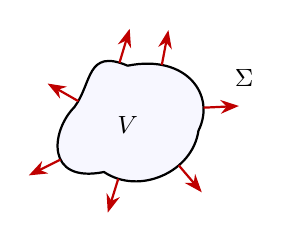
\begin{tikzpicture}[scale=.75]\draw[thick,fill=blue!3,postaction={decorate},decoration={markings,mark=between positions .08 and .98 step .15 with {\draw[cur](0,0)--(0,.45);}}](0,1)..controls(1,1.2)and(1.5,.5)..(1.2,-.1)..controls(1.1,-.8)and(.2,-1.2)..(-.4,-.8)..controls(-1.4,-1)and(-1.3,-.1)..(-.9,.3)..controls(-.6,.7)and(-.7,1.3)..(0,1);\node at(0,0){$V$};\node[right]at(1.65,.8){$\Sigma$};\end{tikzpicture}}
\newcommand{\equipot}{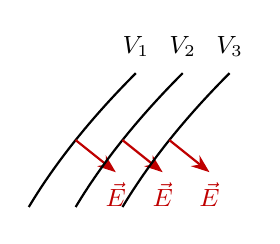
\begin{tikzpicture}[scale=.85]\foreach\k/\lab in{0/1,1/2,2/3}{\draw[thick,domain=-1:1,samples=30]plot({.8*\x+.1*\x*\x+.7*\k},\x);\node[above]at({.9+.7*\k},1.1){$V_\lab$};\draw[cur]({.7*\k},0)--({.7*\k+.6},-.48)node[below]{$\E$};}\end{tikzpicture}}
\newcommand{\potentialsym}[1]{\begin{tikzpicture}[scale=.8]\draw(0,-1)--(0,1.5)node[above]{$\Pi\ifnum#1=1'\fi$};\draw[dotted](-1,0)--(1,0);\node[pt]at(-1,0){};\node[pt]at(1,0){};\node[below]at(-1,-.1){$M$};\node[right]at(1.18,-.16){$M'$};\node[below right]at(0,0){$H$};\draw[cur](-1,0)--(-1.6,1)node[above]{$\E(M)$};\ifnum#1=0\draw[cur](1,0)--(1.6,1)node[above]{$\E(M')$};\draw[green!50!black,->](-1,0)--(-.1,0);\draw[green!50!black,->](1,0)--(.1,0);\else\draw[cur](1,0)--(.4,-1)node[below]{$\E(M')$};\fi\end{tikzpicture}}
\newcommand{\radial}[1]{\begin{tikzpicture}[scale=.75]\draw[green!50!black](0,0)circle(1);\node[below]at(0,-1.9){$q\ifnum#1=1>\else<\fi0$};\fill(0,0)circle(.05);\foreach\a in{15,75,135,195,255,315}{\ifnum#1=1\draw[cur](\a:.25)--(\a:1.7);\else\draw[cur](\a:1.7)--(\a:.25);\fi}\node[green!50!black,above]at(0,1.8){$V=\cste$};\end{tikzpicture}}
\newcommand{\fieldtube}{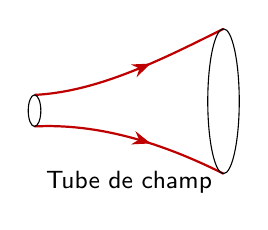
\begin{tikzpicture}[scale=.8]\draw[field](0,-.25)..controls(1,-.2)and(2,-.5)..(3,-1);\draw[field](0,.25)..controls(1,.3)and(2,.8)..(3,1.3);\draw(0,0)ellipse(.1 and .25);\draw(3,.15)ellipse(.25 and 1.15);\node[below]at(1.5,-.8){Tube de champ};\end{tikzpicture}}
\BeforeBeginEnvironment{exemple}{\Needspace{45mm}}
\begin{document}
{\raggedright\fontsize{27}{31}\selectfont\bfseries Électrostatique\par}
\planpart{I}{Champ et potentiel électrostatiques}
\plansub{1}{Propriétés de symétrie}
\plansub{2}{Potentiel scalaire}
\plansubsub{a) Existence d'un potentiel}
\plansubsub{b) Équations de Poisson et de Laplace}
\plansub{3}{Théorème de Gauss}
\plansub{4}{Propriétés topographiques}
\plansubsub{a) Lignes de champ et équipotentielles}
\plansubsub{b) Norme de E dans un tube de champ}
\planpart{II}{Champ et potentiel créés par une distribution de charges}
\plansub{1}{Champ et potentiel créés par une charge ponctuelle}
\plansub{2}{Champ et potentiel créés par une distribution quelconque}
\plansub{3}{Quelques exemples de cartes de champs}
\planpart{III}{Énergie potentielle d'interaction électrostatique}
\plansub{1}{Charge dans un champ extérieur}
\plansub{2}{Énergie potentielle d'interaction d'un système de charges}
\plansubsub{a) Entre deux charges}
\plansubsub{b) Ensemble de N charges}
\plansub{3}{Énergie de constitution}
\planpart{IV}{Exemples de quelques champs électrostatiques}
\plansub{1}{Sphère uniformément chargée}
\plansub{2}{Cylindre infini uniformément chargé}
\plansub{3}{Plan infini uniformément chargé}
\plansub{4}{Condensateur plan}
\plansubsub{a) Conducteurs}
\plansubsub{b) Définition d'un condensateur}
\plansubsub{c) Modèle du condensateur plan}
\planpart{V}{Analogie avec le champ gravitationnel}
\plansub{1}{Champ et potentiel gravitationnels créés par une masse ponctuelle}
\plansub{2}{Champ et potentiel gravitationnels créés par une distribution de masses}
\plansub{3}{Énergie de constitution pour une distribution de masses}
\plansub{4}{Différences entre électrostatique et gravitation}
\vspace{3mm}
% Sources 1--5
La distribution des charges est indépendante du temps : $\D=\{\rho(P)\}\longrightarrow\E(M)$.

On se place à l'échelle mésoscopique avec l'approximation des milieux continus.
Toute l'électrostatique est contenue dans deux équations de Maxwell, auxquelles s'ajoute la force de Lorentz :
\begin{result}\[\divg\E=\frac{\rho}{\eps},\qquad\rot\E=\vec0.\]\end{result}
\titr{Introduction expérimentale}
Il existe trois méthodes de charge.
\titr{Par frottements : effet triboélectrique}
\begin{exemple}\examtitle{1) Ballon chargé par frottements}\fig{\balloon{0}}\end{exemple}
\begin{exemple}\examtitle{2) Paille chargée par frottements}
\fig{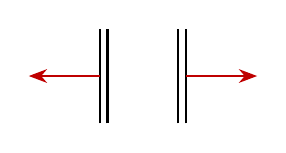
\begin{tikzpicture}\draw[thick](-.5,-.6)--(-.5,.6)(-.4,-.6)--(-.4,.6)(.5,-.6)--(.5,.6)(.6,-.6)--(.6,.6);\draw[cur](-.5,0)--(-1.4,0);\draw[cur](.6,0)--(1.5,0);\end{tikzpicture}}
\end{exemple}
\begin{exemple}\examtitle{3) Verre chargé par frottements}
\fig{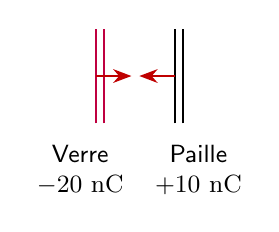
\begin{tikzpicture}\draw[purple,thick](-.5,-.6)--(-.5,.6)(-.4,-.6)--(-.4,.6);\draw[thick](.5,-.6)--(.5,.6)(.6,-.6)--(.6,.6);\draw[cur](-.5,0)--(-.05,0);\draw[cur](.5,0)--(.05,0);\node[below,align=center]at(-.7,-.75){Verre\\$-20\ \mathrm{nC}$};\node[below,align=center]at(.8,-.75){Paille\\$+10\ \mathrm{nC}$};\end{tikzpicture}}
Les charges sont de signes différents.
\end{exemple}
\titr{Par influence}
\fig{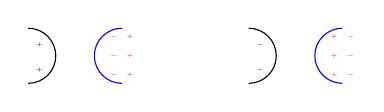
\begin{tikzpicture}\begin{scope}[scale=.7,every node/.style={font=\tiny,inner sep=.5pt}]
\foreach\x/\sg/\opp in{0/+/-,4/-/+}{\draw(\x,0)arc(-90:90:.5);\node at(\x+.2,.25){\scalebox{.45}{$\sg$}};\node at(\x+.2,.7){\scalebox{.45}{$\sg$}};\draw[blue](\x+1.7,0)arc(270:90:.5);\foreach\y in{.15,.5,.85}{\node[red,font=\tiny]at(\x+1.55,\y){\scalebox{.45}{$\opp$}};\node[red,font=\tiny]at(\x+1.85,\y){\scalebox{.45}{$\sg$}};}}\end{scope}\end{tikzpicture}}
\begin{exemple}\examtitle{4) Ballon attiré}\fig{\balloon{1}}La main est chargée par influence.\end{exemple}
\begin{exemple}\examtitle{5) Pendule et objet chargé}
\fig{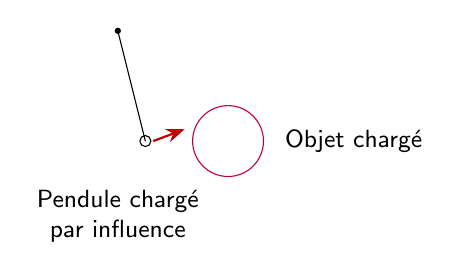
\begin{tikzpicture}\fill(0,1.4)circle(.04);\draw(0,1.4)--(.35,0);\draw(.35,0)circle(.07);\draw[purple](1.4,0)circle(.45);\draw[cur](.45,0)--(.85,.15);\node[below,align=center]at(0,-.5){Pendule chargé\\par influence};\node[right,align=center]at(2,0){Objet chargé};\end{tikzpicture}}\end{exemple}
\begin{exemple}\examtitle{6) Ballons collés au plafond}
\fig{\begin{tikzpicture}\draw(-1.8,.8)--(1.8,.8);\draw[purple](0,.25)circle(.5);\foreach\x in{-.3,0,.3}{\node[red,font=\tiny]at(\x,.95){\scalebox{.45}{$+$}};\node[red,font=\tiny]at(\x,1.4){\scalebox{.45}{$-$}};\node[purple,font=\tiny]at(\x,.3){\scalebox{.45}{$-$}};}\node[purple,font=\tiny]at(0,0){\scalebox{.45}{$-$}};\end{tikzpicture}}\end{exemple}
\begin{exemple}\examtitle{7) Électroscope}\fig{\electroscope{0}}L'électroscope est chargé par influence.\end{exemple}
\titr{Par contact}
\begin{exemple}\examtitle{8) Électroscope chargé par contact}\fig{\electroscope{1}\qquad$\longrightarrow$\qquad\electroscope{2}}\end{exemple}
\begin{exemple}\examtitle{9) Flying stick}
\fig{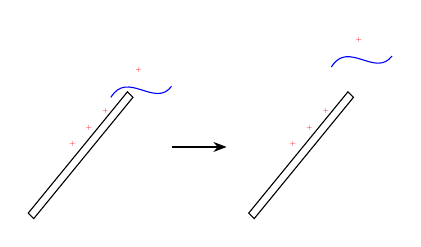
\begin{tikzpicture}[scale=.7]\foreach\x/\h in{0/0,4/.55}{\draw(\x,0)--(\x+1.8,2.2)--(\x+1.9,2.1)--(\x+.1,-.1)--cycle;\draw[blue](\x+1.5,{2.1+\h})..controls(\x+1.8,{2.6+\h})and(\x+2.3,{1.9+\h})..(\x+2.6,{2.3+\h});\foreach\k in{1,1.3,1.6}{\node[red,font=\tiny]at(\x+\k-.2,\k+.25){\scalebox{.45}{$+$}};}\node[red,font=\tiny]at(\x+2,{2.6+\h}){\scalebox{.45}{$+$}};}\draw[->](2.6,1.2)--(3.6,1.2);\end{tikzpicture}}\end{exemple}
\begin{exemple}\examtitle{10) Machine de Wimshurst}
Le champ d'ionisation de l'air est de $10^6\ \mathrm{V\,m^{-1}}$.
\end{exemple}
\begin{exemple}\examtitle{11) Cloche de Franklin}
\fig{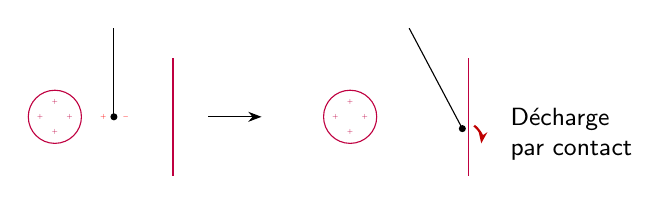
\begin{tikzpicture}\begin{scope}[scale=.75]
\foreach\x in{0,5}{\draw[purple](\x-1,0)circle(.45);\foreach\a in{0,90,180,270}{\node[purple,font=\tiny]at({\x-1+.25*cos(\a)},{.25*sin(\a)}){\scalebox{.45}{$+$}};}\draw[purple](\x+1,-1)--(\x+1,1);}
\draw(0,1.5)--(0,0);\fill(0,0)circle(.06);\node[red,font=\tiny]at(-.18,0){\scalebox{.45}{$+$}};\node[red,font=\tiny]at(.2,0){\scalebox{.45}{$-$}};
\draw(5,1.5)--(5.9,-.2);\fill(5.9,-.2)circle(.06);\draw[cur,-{Stealth[length=1.5mm]}](6.1,-.15)to[bend left](6.22,-.45);\draw[->](1.6,0)--(2.5,0);\node[right,align=left]at(6.55,-.3){Décharge\\par contact};\end{scope}\end{tikzpicture}}\end{exemple}
% Sources 6--17
\section{Champ et potentiel électrostatiques}
\subsection{Propriétés de symétrie}
\[\divg\E=\frac\rho\eps.\]
Un plan $(\Pi)$ de symétrie de $\{\rho\}$ est un plan de symétrie de $\{\E\}$. Il en est de même pour un plan $(\Pi')$ d'antisymétrie.
\begin{result}
Un plan de symétrie d'une distribution de charges (respectivement d'antisymétrie) est un plan de symétrie du champ $\E$ (respectivement d'antisymétrie).
\end{result}
\begin{cadre}En un point d'un plan de symétrie d'une distribution de charges, le champ $\E$ est contenu dans ce plan.

En un point d'un plan d'antisymétrie d'une distribution de charges, le champ $\E$ y est perpendiculaire.\end{cadre}
\subsection{Potentiel scalaire}
\subsubsection{Existence d'un potentiel}
\[\rot\E=\vec0\quad\Longleftrightarrow\quad\E\text{ est à circulation conservative}\quad\Longleftrightarrow\quad\exists V(M)\text{ tel que :}\]
\begin{result}\[\E=-\grad V.\]\end{result}
$V$ est le potentiel scalaire. Unité : $\mathrm V$ (volt).
\titr{Remarques}
\begin{itemize}
\item En travaux pratiques, le multimètre mesure une différence de potentiel $V$.
\item Le potentiel est défini à une constante près, d'où l'importance de la masse en travaux pratiques.
\item On admet que le potentiel est une fonction continue de l'espace. Le champ électrique peut avoir des discontinuités.
\item $\E=-\grad V$.
\end{itemize}
\fig{\equipot}
$V_1>V_2>V_3$. Le champ $\E$ est perpendiculaire à une surface équipotentielle, dans le sens des potentiels décroissants.
\titr{Circulation de $\E$ de $A$ à $B$}
\fig{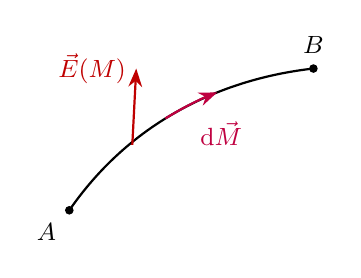
\begin{tikzpicture}\draw[thick](-1.5,-.7)..controls(-.6,.6)and(.7,1)..(1.6,1.1);
\node[pt,label=below left:$A$]at(-1.5,-.7){};\node[pt,label=above:$B$]at(1.6,1.1){};
\draw[cur](-.7,.13)--(-.65,1.1)node[left]{$\E(M)$};
\draw[el](-0.279200,0.466400)..controls(-0.060800,0.601600)and(0.160800,0.710400)..(0.379200,0.797600);
\node[purple,below right]at(.04,.55){$\dM$};\end{tikzpicture}}
\[\int_A^B\E\cdot\dM=-\int_A^B\underbrace{\grad V\cdot\dM}_{=\dd V}.\]
\begin{cadre}\[\int_A^B\E\cdot\dM=V(A)-V(B).\]\end{cadre}
\[W_{A\to B}(q\E)=\int_A^B q\E\cdot\dM=q\bigl(V(A)-V(B)\bigr).\]
Ce travail ne dépend pas du chemin suivi : $q\E$ est conservative et $E_p=qV+\cste$.
\titr{Propriétés de symétrie de $V$}
\[\E=-\grad V.\]
A priori, un plan $(\Pi)$ de symétrie de $\E$ est un plan de symétrie de $V$, et un plan $(\Pi')$ d'antisymétrie de $\E$ est un plan d'antisymétrie de $V$, mais à une constante près, qui dépend de la référence de $V$.
\textbf{Plan de symétrie de $\D$ et de $\E$}\fig{\potentialsym{0}}
\[\int_M^H\E\cdot\dM=\int_{M'}^H\E\cdot\dM.\]
\[V(M)-V(H)=V(M')-V(H).\]
\begin{cadre}\[V(M)=V(M').\]\end{cadre}
$(\Pi)$ est un plan de symétrie pour $V$.

\textbf{Plan d'antisymétrie de $\D$ et de $\E$}\fig{\potentialsym{1}}
\[\int_H^M\E\cdot\dM=\int_{M'}^H\E\cdot\dM.\]
\[V(H)-V(M)=V(M')-V(H).\]
\begin{cadre}\[V(M')-V(H)=-\bigl(V(M)-V(H)\bigr).\]\end{cadre}
$(\Pi')$ est un plan d'antisymétrie pour $V-V(H)$. Souvent, on fixe $V(H)=0$ ; $(\Pi')$ est alors un plan d'antisymétrie pour $V$.

\subsubsection{Équations de Poisson et de Laplace}
\[\divg\E=\frac\rho\eps,\qquad\rot\E=\vec0\quad\Longrightarrow\quad\E=-\grad V.\]
D'où $\divg(-\grad V)=\rho/\eps$.
\begin{result}\[\Delta V+\frac\rho\eps=0.\]\textbf{Équation de Poisson}\end{result}
S'il n'y a pas de charges, $\rho=0$ :
\begin{result}\[\Delta V=0.\]\textbf{Équation de Laplace}\end{result}
\titr{Remarques}
\begin{itemize}\item En mécanique des fluides, on retrouve des équations analogues pour un écoulement parfait, stationnaire et irrotationnel (cf. aile d'avion).
\item Ces équations donnent une méthode pour trouver $V$, puis $\E$, mais il faut connaître les conditions aux limites.\end{itemize}
\subsection{Théorème de Gauss}
On cherche une formulation intégrale, macroscopique, de $\divg\E=\rho/\eps$.
\fig{\blobgauss}
$\Sigma$ est une surface fermée, fixe et indéformable, orientée vers l'extérieur.
\begin{align*}
\oiint_\Sigma\E\cdot\dS&=\iiint_V\divg\E\,\dd^3\tau &&\text{(Green-Ostrogradski)}\\
&=\iiint_V\frac{\rho(P)}\eps\dd^3\tau
=\frac1\eps\iiint_V\rho(P)\dd^3\tau=\frac{Q_{\mathrm{int}}}\eps.
\end{align*}
\begin{result}[5]\textbf{Théorème de Gauss}\[\oiint_\Sigma\E\cdot\dS=\frac{Q_{\mathrm{int}}}\eps.\]
$\Sigma$ est une surface fermée orientée vers l'extérieur. $Q_{\mathrm{int}}$ est la charge totale contenue à l'intérieur de $\Sigma$.\end{result}
\titr{Remarques}
\begin{itemize}\item Ce théorème est utile pour calculer le champ électrique de distributions de haute symétrie.
\item Si, en un point $M$, on a un maximum local de $V$, alors $\oiint_\Sigma\E\cdot\dS=Q_{\mathrm{int}}/\eps>0$.
\end{itemize}
\fig{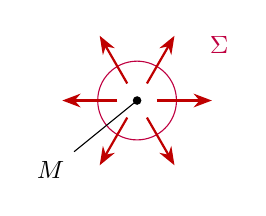
\begin{tikzpicture}\draw[purple](0,0)circle(.5);\node[pt]at(0,0){};\foreach\a in{0,60,...,300}{\draw[cur](\a:.25)--(\a:.95);}\draw[thin](0,0)--(-.8,-.65);\node[below left]at(-.8,-.65){$M$};\node[purple,right]at(.8,.7){$\Sigma$};\end{tikzpicture}}
Alors, en $M$, la charge est positive. Réciproquement, si l'on a un minimum local, la charge est négative.
\subsection{Propriétés topographiques}
\subsubsection{Lignes de champ et équipotentielles}
\begin{itemize}\item $\E=-\grad V$ : les surfaces équipotentielles sont perpendiculaires aux lignes de champ, orientées dans le sens des potentiels décroissants.
\item Dans une ligne de champ, $\E(M)\parallel\dM$. Les équations des lignes de champ sont :\end{itemize}
\[\frac{\dd x}{E_x}=\frac{\dd y}{E_y}=\frac{\dd z}{E_z},\qquad
\frac{\dd r}{E_r}=\frac{r\dd\theta}{E_\theta}=\frac{\dd z}{E_z},\qquad
\frac{\dd r}{E_r}=\frac{r\dd\theta}{E_\theta}=\frac{r\sin\theta\dd\varphi}{E_\varphi}.\]
Si deux lignes de champ se coupent en $A$, alors $\E(A)=\vec0$.
\fig{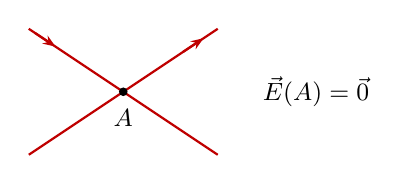
\begin{tikzpicture}\draw[red!75!black,thick](-1.2,-.8)--(0,0)--(1.2,.8);
\draw[cur,-{Stealth[length=1.6mm]}](.76,.506667)--(1.02,.68);
\draw[red!75!black,thick](-1.2,.8)--(0,0)--(1.2,-.8);
\draw[cur,-{Stealth[length=1.6mm]}](-1.12,.746667)--(-.86,.573333);
\node[pt]at(0,0){};\node[below,yshift=-3pt]at(0,0){$A$};\node[right]at(1.65,0){$\E(A)=\vec0$};\end{tikzpicture}}
Une ligne de champ électrostatique ne peut pas être fermée. Par l'absurde, supposons qu'une telle ligne existe.
\fig{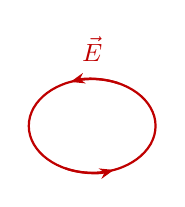
\begin{tikzpicture}[scale=.7]
\draw[red!75!black,thick](0,0)ellipse(1.15 and .85);
\draw[cur,-{Stealth[length=1.8mm]}](65:1.15 and .85)arc(65:110:1.15 and .85);
\draw[cur,-{Stealth[length=1.8mm]}](245:1.15 and .85)arc(245:290:1.15 and .85);
\node[red!75!black,above]at(0,1){$\E$};\end{tikzpicture}}
Alors $\displaystyle\oint_{A\to A}\E\cdot\dM>0$, ce qui est impossible car $\E$ est à circulation conservative.

Pour deux surfaces équipotentielles proches :
\fig{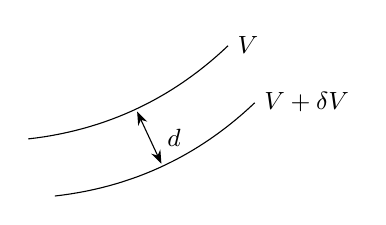
\begin{tikzpicture}\begin{scope}[rotate=25]
\draw[domain=-1.4:1.4,samples=30]plot(\x,{.12*\x*\x+.4});
\draw[domain=-1.4:1.4,samples=30]plot(\x,{.12*\x*\x-.4});
\draw[<->,shorten <=1pt,shorten >=1pt](0,-.4)--(0,.4)node[midway,right=3pt]{$d$};
\node[right]at(1.4,.64){$V$};\node[right]at(1.4,-.16){$V+\delta V$};\end{scope}\end{tikzpicture}}
\[E\simeq\frac{\delta V}{d}.\]
\subsubsection{Norme de E dans un tube de champ}
Dans une région vide de charges, $\rho(M)=0$ et $\divg\E=0$ : $\E$ est à flux conservatif.
\fig{\fieldtube}
\begin{cadre}
Dans une région vide de charges, le champ $\E$ est à flux conservatif. Il y a donc conservation du flux de $\E$ à travers toute section du tube de champ.

Si les lignes de champ s'éloignent, la norme de $\E$ diminue ; si les lignes de champ se resserrent, la norme de $\E$ augmente.
\end{cadre}
% Sources 17--24
\section{Champ et potentiel créés par une distribution de charges}
\subsection{Champ et potentiel créés par une charge ponctuelle}
Les équations de Maxwell sont linéaires : connaître le champ créé par une charge ponctuelle permet de déterminer celui de toute distribution.
\fig{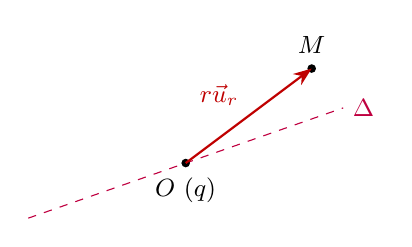
\begin{tikzpicture}\draw[purple,dashed](-2,-.7)--(2,.7)node[right]{$\Delta$};\node[pt,label=below:$O\ (q)$]at(0,0){};\node[pt,label=above:$M$]at(1.6,1.2){};\draw[cur](0,0)--(1.6,1.2)node[midway,above left]{$r\ur$};\end{tikzpicture}}
Dans la base sphérique,
\[\E(M)=E_r(r,\theta,\varphi)\ur+E_\theta(r,\theta,\varphi)\ut+E_\varphi(r,\theta,\varphi)\uphi.\]
La symétrie sphérique correspond à l'invariance par rotation autour de tout axe $\Delta$ passant par $O$ : le champ ne dépend que de $r$.
Tous les plans contenant $OM$ sont des plans de symétrie de la distribution et du champ. Comme $M$ appartient à chacun de ces plans, $\E(M)$ leur est parallèle. Ainsi,
\[\E(M)=E_r(r)\ur.\]
\fig{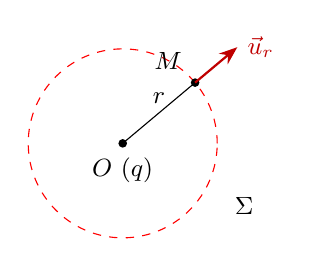
\begin{tikzpicture}\draw[red,dashed](0,0)circle(1.2);\node[pt,label=below:$O\ (q)$]at(0,0){};\draw(0,0)--(40:1.2)node[midway,above]{$r$};\node[pt,label=above left:$M$]at(40:1.2){};\draw[cur](40:1.2)--(40:1.9)node[right]{$\ur$};\node[right]at(1.3,-.8){$\Sigma$};\end{tikzpicture}}
La surface de Gauss est la sphère de centre $O$ passant par $M$, orientée vers l'extérieur.
\[\oiint_\Sigma\E\cdot\dS=\frac{Q_{\mathrm{int}}}{\eps}=\frac q\eps.\]
Or,
\[\oiint_\Sigma\E\cdot\dS=\oiint_\Sigma E_r(r)\ur\cdot\dd^2S\ur
=E_r(r)\oiint_\Sigma\dd^2S=4\pi r^2E_r(r).\]
\begin{result}\[\E(M)=\frac{q}{4\pi\eps r^2}\ur,\qquad V(M)=\frac{q}{4\pi\eps r}+\cste.\]\end{result}
\fig{\radial{1}\hspace{2cm}\radial{0}}
\subsection{Champ et potentiel créés par une distribution quelconque}
\titr{Première méthode : théorème de superposition}
Les équations de Maxwell sont linéaires.
\titr{Distribution de charges ponctuelles}
\fig{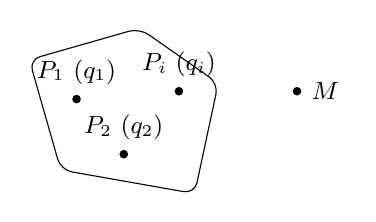
\begin{tikzpicture}\draw[rounded corners](0,0)--(-.4,1.4)--(1,1.8)--(2,1.1)--(1.7,-.3)--cycle;\foreach\x/\y/\l in{.2/.9/1,.8/.2/2,1.5/1/i}{\node[pt,label=above:{$P_\l\ (q_\l)$}]at(\x,\y){};}\node[pt,label=right:$M$]at(3,1){};\end{tikzpicture}}
\begin{result}[2]\[\E(M)=\sum_i\frac{q_i\overrightarrow{P_iM}}{4\pi\eps P_iM^3},\qquad V(M)=\sum_i\frac{q_i}{4\pi\eps P_iM}+\cste.\]\end{result}
Le choix $V\to0$ lorsque $r\to\infty$ impose une constante nulle.
\titr{Distribution volumique}
\fig{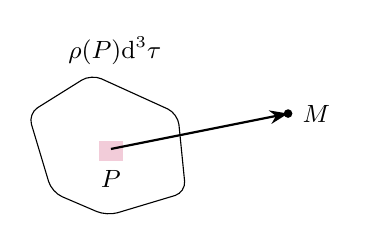
\begin{tikzpicture}\draw[rounded corners](0,0)--(-.3,1)--(.5,1.5)--(1.6,1)--(1.7,0)--(.7,-.3)--cycle;\fill[purple!20](.6,.4)rectangle(.9,.65);\node[below]at(.75,.4){$P$};\node[above]at(.8,1.5){$\rho(P)\dd^3\tau$};\node[pt,label=right:$M$]at(3,1){};\draw[arr](.75,.55)--(3,1);\end{tikzpicture}}
\begin{result}[2]\[\E(M)=\iiint_{\mathcal V}\frac{\rho(P)\dd^3\tau}{4\pi\eps PM^3}\overrightarrow{PM},\qquad V(M)=\iiint_{\mathcal V}\frac{\rho(P)\dd^3\tau}{4\pi\eps PM}.\]\end{result}
\titr{Distribution surfacique}
\fig{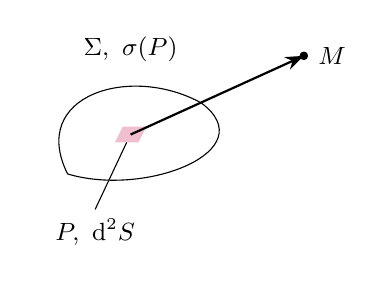
\begin{tikzpicture}\draw(0,0)..controls(-.5,1)and(.8,1.4)..(1.7,.9)..controls(2.5,.3)and(1,-.3)..cycle;\fill[purple!25](.6,.4)--(.9,.4)--(1,.6)--(.7,.6)--cycle;\draw[thin](.75,.4)--(.35,-.45);\node[below]at(.35,-.45){$P,\ \dd^2S$};\node[above]at(.8,1.3){$\Sigma,\ \sigma(P)$};\node[pt,label=right:$M$]at(3,1.5){};\draw[arr](.8,.5)--(3,1.5);\end{tikzpicture}}
\begin{result}[2]\[\E(M)=\iint_\Sigma\frac{\sigma(P)\dd^2S}{4\pi\eps PM^3}\overrightarrow{PM},\qquad V(M)=\iint_\Sigma\frac{\sigma(P)\dd^2S}{4\pi\eps PM}.\]\end{result}
\titr{Distribution linéique}
\fig{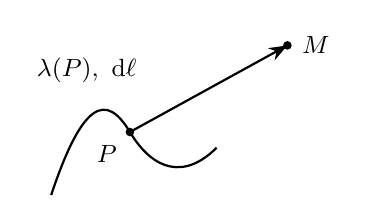
\begin{tikzpicture}\draw[thick](0,-.3)..controls(.4,.9)and(.7,1)..(1,.5)..controls(1.3,0)and(1.7,-.1)..(2.1,.3);
\node[pt,label=below left:$P$]at(1,.5){};\node[above]at(.45,1){$\lambda(P),\ \dd\ell$};\node[pt,label=right:$M$]at(3,1.6){};\draw[arr](1,.5)--(3,1.6);\end{tikzpicture}}
\begin{result}[2]\[\E(M)=\int_\D\frac{\lambda(P)\dd\ell}{4\pi\eps PM^3}\overrightarrow{PM},\qquad V(M)=\int_\D\frac{\lambda(P)\dd\ell}{4\pi\eps PM}.\]\end{result}
\titr{Point méthode}
Cette méthode calculatoire est à éviter, mais elle reste utile, en particulier pour les charges ponctuelles. Les symétries et invariances sont essentielles pour simplifier le champ avant tout calcul intégral.
Quatre méthodes sont au programme ; les symétries et invariances restent essentielles dans tous les cas.
\begin{enumerate}
\item Le théorème de Gauss, $\oiint\E\cdot\dS=Q_{\mathrm{int}}/\eps$, convient aux problèmes de haute symétrie. On choisit une surface sur laquelle le champ est partout parallèle ou perpendiculaire à la surface.
\item On intègre $\divg\E=\rho/\eps$, puis on détermine les constantes d'intégration.
\item L'équation de Poisson $\Delta V+\rho/\eps=0$ est une équation aux dérivées partielles d'ordre deux. On l'intègre deux fois, en utilisant la continuité de $V$.
\item La superposition ne se limite pas aux charges ponctuelles : on peut décomposer la distribution en distributions connues, pas nécessairement ponctuelles.
\end{enumerate}
La démarche inverse est également possible : déterminer la distribution à partir du champ ou du potentiel.
\subsection{Quelques exemples de cartes de champs}
\titr{Champ uniforme}
\fig{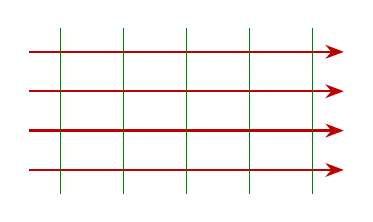
\begin{tikzpicture}\foreach\y in{0,.5,1,1.5}{\draw[cur](0,\y)--(4,\y);}\foreach\x in{.4,1.2,2,2.8,3.6}{\draw[green!50!black](\x,-.3)--(\x,1.8);}\end{tikzpicture}}
\Needspace{65mm}\titr{Charge positive dans un champ uniforme}
\fig{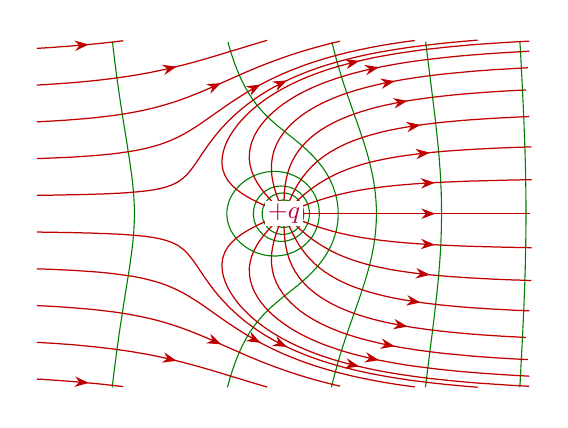
\begin{tikzpicture}[scale=1.05]
\clip (-3.1,-2.25) rectangle (3.1,2.25);
\draw[green!50!black,thin] plot coordinates {(2.853,-2.100) (2.855,-2.056) (2.857,-2.033) (2.859,-1.989) (2.861,-1.944) (2.864,-1.900) (2.866,-1.856) (2.868,-1.811) (2.871,-1.767) (2.873,-1.722) (2.875,-1.678) (2.878,-1.633) (2.880,-1.599) (2.881,-1.567) (2.883,-1.522) (2.886,-1.478) (2.888,-1.433) (2.890,-1.389) (2.892,-1.344) (2.894,-1.300) (2.896,-1.256) (2.898,-1.211) (2.900,-1.167) (2.902,-1.122) (2.904,-1.078) (2.904,-1.056) (2.906,-1.011) (2.908,-0.967) (2.910,-0.922) (2.911,-0.878) (2.913,-0.833) (2.914,-0.789) (2.915,-0.744) (2.917,-0.700) (2.918,-0.656) (2.919,-0.611) (2.920,-0.567) (2.921,-0.522) (2.922,-0.478) (2.923,-0.433) (2.924,-0.389) (2.924,-0.344) (2.925,-0.300) (2.926,-0.256) (2.926,-0.211) (2.926,-0.167) (2.927,-0.122) (2.927,-0.078) (2.927,-0.033) (2.927,0.011) (2.927,0.056) (2.927,0.100) (2.927,0.144) (2.926,0.189) (2.926,0.233) (2.925,0.278) (2.925,0.322) (2.924,0.367) (2.923,0.411) (2.923,0.456) (2.922,0.500) (2.921,0.544) (2.920,0.589) (2.919,0.633) (2.917,0.678) (2.916,0.722) (2.915,0.767) (2.913,0.811) (2.912,0.856) (2.910,0.900) (2.909,0.944) (2.907,0.989) (2.905,1.033) (2.904,1.077) (2.903,1.100) (2.901,1.144) (2.899,1.189) (2.897,1.233) (2.895,1.278) (2.893,1.322) (2.891,1.367) (2.889,1.411) (2.887,1.456) (2.884,1.500) (2.882,1.544) (2.880,1.589) (2.879,1.611) (2.877,1.656) (2.874,1.700) (2.872,1.744) (2.870,1.789) (2.867,1.833) (2.865,1.878) (2.863,1.922) (2.860,1.967) (2.858,2.011) (2.855,2.053) (2.854,2.078)};
\draw[green!50!black,thin] plot coordinates {(1.711,-2.100) (1.717,-2.056) (1.722,-2.011) (1.725,-1.989) (1.730,-1.944) (1.736,-1.900) (1.741,-1.856) (1.747,-1.811) (1.750,-1.789) (1.755,-1.744) (1.761,-1.700) (1.766,-1.656) (1.771,-1.618) (1.775,-1.589) (1.780,-1.544) (1.786,-1.500) (1.792,-1.456) (1.795,-1.426) (1.800,-1.389) (1.805,-1.344) (1.811,-1.300) (1.816,-1.256) (1.819,-1.229) (1.824,-1.189) (1.829,-1.144) (1.834,-1.100) (1.839,-1.056) (1.843,-1.020) (1.847,-0.989) (1.851,-0.944) (1.856,-0.900) (1.860,-0.856) (1.865,-0.811) (1.867,-0.781) (1.871,-0.744) (1.875,-0.700) (1.878,-0.656) (1.882,-0.611) (1.885,-0.567) (1.888,-0.522) (1.891,-0.478) (1.892,-0.456) (1.895,-0.411) (1.897,-0.367) (1.899,-0.322) (1.901,-0.278) (1.902,-0.233) (1.904,-0.189) (1.904,-0.144) (1.905,-0.100) (1.906,-0.056) (1.906,-0.011) (1.906,0.033) (1.905,0.078) (1.905,0.122) (1.904,0.167) (1.903,0.211) (1.902,0.256) (1.900,0.300) (1.898,0.344) (1.896,0.389) (1.894,0.433) (1.892,0.467) (1.890,0.500) (1.887,0.544) (1.883,0.589) (1.880,0.633) (1.877,0.678) (1.873,0.722) (1.869,0.767) (1.867,0.789) (1.863,0.833) (1.858,0.878) (1.854,0.922) (1.849,0.967) (1.844,1.011) (1.842,1.033) (1.837,1.078) (1.832,1.122) (1.827,1.167) (1.821,1.211) (1.819,1.233) (1.813,1.278) (1.808,1.322) (1.803,1.367) (1.797,1.411) (1.794,1.433) (1.789,1.478) (1.783,1.522) (1.778,1.567) (1.772,1.611) (1.769,1.633) (1.764,1.678) (1.758,1.722) (1.752,1.767) (1.747,1.809) (1.744,1.833) (1.738,1.878) (1.733,1.922) (1.728,1.967) (1.723,2.005) (1.719,2.033) (1.714,2.078)};
\draw[green!50!black,thin] plot coordinates {(0.574,-2.100) (0.585,-2.056) (0.590,-2.033) (0.602,-1.989) (0.613,-1.944) (0.619,-1.922) (0.631,-1.878) (0.639,-1.851) (0.650,-1.811) (0.662,-1.767) (0.669,-1.744) (0.682,-1.700) (0.689,-1.678) (0.703,-1.633) (0.711,-1.608) (0.724,-1.567) (0.735,-1.534) (0.746,-1.500) (0.759,-1.462) (0.769,-1.433) (0.783,-1.391) (0.791,-1.367) (0.807,-1.322) (0.815,-1.300) (0.830,-1.256) (0.838,-1.233) (0.854,-1.189) (0.862,-1.167) (0.877,-1.122) (0.885,-1.100) (0.901,-1.056) (0.908,-1.033) (0.924,-0.989) (0.931,-0.967) (0.946,-0.922) (0.953,-0.900) (0.968,-0.856) (0.976,-0.830) (0.988,-0.789) (1.000,-0.750) (1.008,-0.722) (1.020,-0.678) (1.026,-0.656) (1.038,-0.611) (1.048,-0.569) (1.054,-0.544) (1.064,-0.500) (1.072,-0.457) (1.077,-0.433) (1.085,-0.389) (1.092,-0.344) (1.096,-0.313) (1.101,-0.278) (1.106,-0.233) (1.110,-0.189) (1.113,-0.144) (1.116,-0.100) (1.117,-0.056) (1.118,-0.011) (1.118,0.033) (1.117,0.078) (1.115,0.122) (1.112,0.167) (1.108,0.211) (1.104,0.256) (1.098,0.300) (1.095,0.322) (1.088,0.367) (1.081,0.411) (1.073,0.456) (1.068,0.478) (1.059,0.522) (1.049,0.567) (1.043,0.589) (1.032,0.633) (1.024,0.664) (1.014,0.700) (1.002,0.744) (0.995,0.767) (0.982,0.811) (0.975,0.833) (0.961,0.878) (0.952,0.905) (0.939,0.944) (0.928,0.977) (0.916,1.011) (0.904,1.047) (0.893,1.078) (0.880,1.116) (0.870,1.144) (0.855,1.185) (0.846,1.211) (0.831,1.253) (0.823,1.278) (0.807,1.321) (0.799,1.344) (0.784,1.389) (0.776,1.411) (0.761,1.456) (0.754,1.478) (0.739,1.522) (0.731,1.544) (0.717,1.589) (0.710,1.611) (0.696,1.656) (0.687,1.686) (0.676,1.722) (0.663,1.766) (0.656,1.789) (0.643,1.833) (0.637,1.856) (0.625,1.900) (0.614,1.939) (0.607,1.967) (0.596,2.011) (0.590,2.033) (0.579,2.078)};
\draw[green!50!black,thin] plot coordinates {(-0.684,-2.100) (-0.672,-2.056) (-0.663,-2.022) (-0.653,-1.989) (-0.639,-1.944) (-0.632,-1.922) (-0.618,-1.878) (-0.610,-1.856) (-0.594,-1.811) (-0.586,-1.789) (-0.569,-1.744) (-0.560,-1.722) (-0.542,-1.681) (-0.531,-1.656) (-0.518,-1.627) (-0.500,-1.589) (-0.488,-1.567) (-0.470,-1.532) (-0.452,-1.500) (-0.439,-1.478) (-0.422,-1.449) (-0.398,-1.412) (-0.382,-1.389) (-0.367,-1.367) (-0.349,-1.343) (-0.325,-1.312) (-0.301,-1.283) (-0.278,-1.256) (-0.258,-1.233) (-0.237,-1.211) (-0.216,-1.189) (-0.193,-1.167) (-0.170,-1.144) (-0.145,-1.122) (-0.120,-1.100) (-0.095,-1.078) (-0.068,-1.056) (-0.041,-1.033) (-0.014,-1.011) (0.012,-0.990) (0.036,-0.971) (0.060,-0.952) (0.084,-0.933) (0.108,-0.914) (0.133,-0.894) (0.157,-0.875) (0.181,-0.855) (0.206,-0.833) (0.232,-0.811) (0.257,-0.789) (0.281,-0.767) (0.304,-0.744) (0.327,-0.722) (0.349,-0.699) (0.373,-0.673) (0.398,-0.646) (0.422,-0.618) (0.444,-0.589) (0.461,-0.567) (0.477,-0.544) (0.494,-0.519) (0.518,-0.481) (0.533,-0.456) (0.545,-0.433) (0.566,-0.391) (0.578,-0.367) (0.590,-0.336) (0.604,-0.300) (0.614,-0.268) (0.625,-0.233) (0.636,-0.189) (0.640,-0.167) (0.648,-0.122) (0.653,-0.078) (0.655,-0.033) (0.656,0.011) (0.654,0.056) (0.650,0.100) (0.644,0.144) (0.639,0.174) (0.630,0.211) (0.618,0.256) (0.611,0.278) (0.596,0.322) (0.587,0.344) (0.567,0.389) (0.557,0.411) (0.542,0.439) (0.520,0.478) (0.506,0.500) (0.492,0.522) (0.470,0.555) (0.446,0.587) (0.427,0.611) (0.409,0.633) (0.389,0.656) (0.369,0.678) (0.349,0.700) (0.325,0.724) (0.301,0.747) (0.277,0.770) (0.253,0.792) (0.229,0.814) (0.205,0.834) (0.180,0.856) (0.153,0.878) (0.125,0.900) (0.098,0.922) (0.070,0.944) (0.042,0.967) (0.014,0.989) (-0.012,1.010) (-0.036,1.029) (-0.060,1.049) (-0.084,1.069) (-0.108,1.090) (-0.133,1.111) (-0.157,1.133) (-0.181,1.155) (-0.205,1.178) (-0.229,1.203) (-0.253,1.228) (-0.277,1.255) (-0.297,1.278) (-0.316,1.300) (-0.333,1.322) (-0.350,1.344) (-0.373,1.376) (-0.397,1.411) (-0.412,1.433) (-0.426,1.456) (-0.446,1.489) (-0.465,1.522) (-0.477,1.544) (-0.494,1.578) (-0.510,1.611) (-0.521,1.633) (-0.541,1.678) (-0.550,1.700) (-0.566,1.738) (-0.577,1.767) (-0.590,1.801) (-0.602,1.833) (-0.614,1.868) (-0.625,1.900) (-0.639,1.942) (-0.646,1.967) (-0.659,2.011) (-0.666,2.033) (-0.678,2.078)};
\draw[green!50!black,thin] plot coordinates {(-2.077,-2.100) (-2.072,-2.056) (-2.067,-2.011) (-2.061,-1.967) (-2.059,-1.944) (-2.053,-1.900) (-2.048,-1.856) (-2.042,-1.811) (-2.036,-1.767) (-2.033,-1.744) (-2.028,-1.700) (-2.022,-1.656) (-2.016,-1.611) (-2.012,-1.586) (-2.006,-1.544) (-2.000,-1.500) (-1.994,-1.456) (-1.988,-1.417) (-1.984,-1.389) (-1.977,-1.344) (-1.970,-1.300) (-1.964,-1.257) (-1.960,-1.233) (-1.953,-1.189) (-1.946,-1.144) (-1.940,-1.102) (-1.936,-1.078) (-1.929,-1.033) (-1.922,-0.989) (-1.916,-0.952) (-1.911,-0.922) (-1.904,-0.878) (-1.897,-0.833) (-1.892,-0.802) (-1.886,-0.767) (-1.879,-0.722) (-1.872,-0.678) (-1.867,-0.646) (-1.862,-0.611) (-1.856,-0.567) (-1.850,-0.522) (-1.844,-0.478) (-1.841,-0.456) (-1.835,-0.411) (-1.830,-0.367) (-1.826,-0.322) (-1.822,-0.278) (-1.819,-0.249) (-1.816,-0.211) (-1.814,-0.167) (-1.812,-0.122) (-1.810,-0.078) (-1.809,-0.033) (-1.809,0.011) (-1.809,0.056) (-1.811,0.100) (-1.813,0.144) (-1.815,0.189) (-1.818,0.233) (-1.820,0.256) (-1.824,0.300) (-1.828,0.344) (-1.833,0.389) (-1.838,0.433) (-1.843,0.475) (-1.847,0.500) (-1.853,0.544) (-1.859,0.589) (-1.866,0.633) (-1.869,0.656) (-1.876,0.700) (-1.883,0.744) (-1.890,0.789) (-1.893,0.811) (-1.900,0.856) (-1.907,0.900) (-1.914,0.944) (-1.918,0.967) (-1.925,1.011) (-1.932,1.056) (-1.939,1.100) (-1.943,1.122) (-1.950,1.167) (-1.957,1.211) (-1.964,1.256) (-1.967,1.278) (-1.974,1.322) (-1.981,1.367) (-1.987,1.411) (-1.990,1.433) (-1.997,1.478) (-2.003,1.522) (-2.009,1.567) (-2.013,1.589) (-2.019,1.633) (-2.025,1.678) (-2.031,1.722) (-2.036,1.765) (-2.039,1.789) (-2.045,1.833) (-2.050,1.878) (-2.056,1.922) (-2.060,1.958) (-2.064,1.989) (-2.069,2.033) (-2.074,2.078)};
\draw[green!50!black,thin] plot coordinates {(-0.229,-0.501) (-0.181,-0.508) (-0.133,-0.511) (-0.084,-0.511) (-0.036,-0.506) (-0.001,-0.500) (0.036,-0.492) (0.080,-0.478) (0.108,-0.467) (0.133,-0.456) (0.175,-0.433) (0.205,-0.414) (0.229,-0.397) (0.253,-0.377) (0.277,-0.355) (0.301,-0.329) (0.325,-0.300) (0.341,-0.278) (0.356,-0.256) (0.373,-0.223) (0.389,-0.189) (0.398,-0.167) (0.412,-0.122) (0.421,-0.078) (0.424,-0.056) (0.427,-0.011) (0.426,0.033) (0.422,0.072) (0.417,0.100) (0.406,0.144) (0.398,0.167) (0.379,0.211) (0.368,0.233) (0.349,0.265) (0.325,0.300) (0.307,0.322) (0.287,0.344) (0.265,0.367) (0.239,0.389) (0.209,0.411) (0.181,0.430) (0.157,0.444) (0.133,0.456) (0.084,0.476) (0.060,0.485) (0.012,0.498) (-0.012,0.502) (-0.060,0.509) (-0.108,0.512) (-0.157,0.510) (-0.205,0.505) (-0.232,0.500) (-0.277,0.489) (-0.314,0.478) (-0.349,0.465) (-0.373,0.454) (-0.414,0.433) (-0.446,0.414) (-0.470,0.398) (-0.494,0.380) (-0.518,0.360) (-0.542,0.337) (-0.566,0.312) (-0.590,0.283) (-0.610,0.256) (-0.624,0.233) (-0.639,0.208) (-0.658,0.167) (-0.666,0.144) (-0.679,0.100) (-0.687,0.059) (-0.690,0.033) (-0.691,-0.011) (-0.687,-0.056) (-0.684,-0.078) (-0.674,-0.122) (-0.663,-0.154) (-0.648,-0.189) (-0.637,-0.211) (-0.614,-0.249) (-0.594,-0.278) (-0.577,-0.300) (-0.557,-0.322) (-0.535,-0.344) (-0.510,-0.367) (-0.482,-0.389) (-0.451,-0.411) (-0.422,-0.429) (-0.398,-0.442) (-0.370,-0.456) (-0.325,-0.474) (-0.301,-0.482) (-0.253,-0.496) (-0.229,-0.501)};
\draw[green!50!black,thin] plot coordinates {(-0.108,-0.326) (-0.060,-0.334) (-0.012,-0.335) (0.036,-0.328) (0.061,-0.322) (0.108,-0.306) (0.133,-0.294) (0.158,-0.278) (0.188,-0.256) (0.212,-0.233) (0.232,-0.211) (0.253,-0.183) (0.275,-0.144) (0.285,-0.122) (0.299,-0.078) (0.303,-0.056) (0.308,-0.011) (0.307,0.033) (0.301,0.066) (0.293,0.100) (0.277,0.140) (0.263,0.167) (0.249,0.189) (0.229,0.215) (0.205,0.241) (0.181,0.262) (0.157,0.279) (0.119,0.300) (0.084,0.315) (0.060,0.323) (0.012,0.332) (-0.036,0.335) (-0.084,0.331) (-0.121,0.322) (-0.157,0.311) (-0.181,0.300) (-0.220,0.278) (-0.249,0.256) (-0.274,0.233) (-0.294,0.211) (-0.311,0.189) (-0.325,0.166) (-0.346,0.122) (-0.355,0.100) (-0.365,0.056) (-0.370,0.011) (-0.368,-0.033) (-0.361,-0.078) (-0.349,-0.114) (-0.337,-0.144) (-0.325,-0.167) (-0.301,-0.202) (-0.277,-0.230) (-0.253,-0.253) (-0.229,-0.271) (-0.205,-0.287) (-0.181,-0.300) (-0.133,-0.319) (-0.108,-0.326)};
\draw[green!50!black,thin] plot coordinates {(-0.084,-0.240) (-0.036,-0.250) (0.012,-0.250) (0.060,-0.240) (0.084,-0.231) (0.122,-0.211) (0.152,-0.189) (0.175,-0.167) (0.193,-0.144) (0.207,-0.122) (0.226,-0.078) (0.233,-0.056) (0.239,-0.011) (0.237,0.033) (0.229,0.068) (0.218,0.100) (0.205,0.125) (0.181,0.160) (0.157,0.185) (0.133,0.205) (0.108,0.220) (0.078,0.233) (0.036,0.246) (-0.012,0.251) (-0.060,0.246) (-0.103,0.233) (-0.133,0.220) (-0.157,0.205) (-0.181,0.186) (-0.205,0.161) (-0.229,0.127) (-0.243,0.100) (-0.253,0.072) (-0.262,0.033) (-0.264,-0.011) (-0.258,-0.056) (-0.252,-0.078) (-0.232,-0.122) (-0.218,-0.144) (-0.200,-0.167) (-0.178,-0.189) (-0.148,-0.211) (-0.108,-0.232) (-0.084,-0.240)};
\draw[green!50!black,thin] plot coordinates {(-0.084,-0.146) (-0.036,-0.164) (0.012,-0.166) (0.060,-0.155) (0.084,-0.142) (0.110,-0.122) (0.133,-0.096) (0.154,-0.056) (0.160,-0.033) (0.163,0.011) (0.157,0.045) (0.144,0.078) (0.130,0.100) (0.108,0.124) (0.079,0.144) (0.036,0.162) (-0.012,0.167) (-0.060,0.157) (-0.087,0.144) (-0.117,0.122) (-0.138,0.100) (-0.157,0.066) (-0.168,0.033) (-0.171,-0.011) (-0.161,-0.056) (-0.152,-0.078) (-0.133,-0.106) (-0.108,-0.130) (-0.084,-0.146)};
\draw[field,line width=.45pt] plot coordinates {(0.120,0.000) (0.195,0.000) (0.270,0.000) (0.345,0.000) (0.420,0.000) (0.495,0.000) (0.570,0.000) (0.645,0.000) (0.720,0.000) (0.795,0.000) (0.870,0.000) (0.945,0.000) (1.020,0.000) (1.095,0.000) (1.170,0.000) (1.245,0.000) (1.320,0.000) (1.395,0.000) (1.470,0.000) (1.545,0.000) (1.620,0.000) (1.695,0.000) (1.770,0.000) (1.845,0.000) (1.920,0.000) (1.995,0.000) (2.070,0.000) (2.145,0.000) (2.220,0.000) (2.295,0.000) (2.370,0.000) (2.445,0.000) (2.520,0.000) (2.595,0.000) (2.670,0.000) (2.745,0.000) (2.820,0.000) (2.895,0.000) (2.970,0.000)};
\draw[field,line width=.45pt] plot coordinates {(0.111,0.046) (0.180,0.074) (0.250,0.101) (0.321,0.127) (0.391,0.152) (0.463,0.175) (0.535,0.197) (0.607,0.217) (0.680,0.235) (0.753,0.252) (0.826,0.267) (0.900,0.281) (0.974,0.294) (1.048,0.305) (1.122,0.315) (1.197,0.325) (1.271,0.333) (1.346,0.341) (1.420,0.348) (1.495,0.354) (1.570,0.360) (1.645,0.365) (1.720,0.370) (1.794,0.374) (1.869,0.378) (1.944,0.382) (2.019,0.385) (2.094,0.388) (2.169,0.391) (2.244,0.394) (2.319,0.396) (2.394,0.398) (2.469,0.400) (2.544,0.402) (2.619,0.404) (2.694,0.406) (2.769,0.407) (2.844,0.409) (2.919,0.410) (2.994,0.411)};
\draw[field,line width=.45pt] plot coordinates {(0.085,0.085) (0.139,0.137) (0.194,0.188) (0.251,0.237) (0.309,0.284) (0.369,0.328) (0.432,0.370) (0.496,0.409) (0.561,0.445) (0.629,0.479) (0.697,0.509) (0.767,0.537) (0.838,0.562) (0.909,0.585) (0.981,0.606) (1.054,0.625) (1.127,0.642) (1.200,0.657) (1.274,0.672) (1.347,0.685) (1.421,0.696) (1.496,0.707) (1.570,0.717) (1.645,0.726) (1.719,0.734) (1.794,0.742) (1.868,0.749) (1.943,0.755) (2.018,0.761) (2.093,0.766) (2.167,0.771) (2.242,0.776) (2.317,0.780) (2.392,0.784) (2.467,0.788) (2.542,0.792) (2.617,0.795) (2.692,0.798) (2.767,0.801) (2.842,0.803) (2.917,0.806) (2.992,0.808)};
\draw[field,line width=.45pt] plot coordinates {(0.046,0.111) (0.076,0.179) (0.109,0.247) (0.144,0.313) (0.182,0.378) (0.225,0.440) (0.271,0.499) (0.321,0.555) (0.374,0.607) (0.431,0.656) (0.491,0.701) (0.554,0.742) (0.618,0.780) (0.685,0.815) (0.753,0.847) (0.822,0.876) (0.892,0.902) (0.963,0.926) (1.035,0.948) (1.107,0.968) (1.180,0.987) (1.253,1.004) (1.326,1.019) (1.400,1.033) (1.474,1.046) (1.548,1.058) (1.622,1.069) (1.696,1.080) (1.771,1.089) (1.845,1.098) (1.920,1.106) (1.994,1.113) (2.069,1.120) (2.144,1.127) (2.219,1.133) (2.293,1.138) (2.368,1.143) (2.443,1.148) (2.518,1.153) (2.593,1.157) (2.668,1.161) (2.743,1.165) (2.817,1.169) (2.892,1.172) (2.967,1.175)};
\draw[field,line width=.45pt] plot coordinates {(0.000,0.120) (0.002,0.195) (0.006,0.270) (0.014,0.344) (0.027,0.418) (0.045,0.491) (0.068,0.562) (0.098,0.631) (0.134,0.697) (0.175,0.760) (0.222,0.818) (0.273,0.873) (0.328,0.924) (0.387,0.970) (0.448,1.013) (0.512,1.053) (0.578,1.089) (0.645,1.123) (0.713,1.153) (0.783,1.182) (0.853,1.207) (0.924,1.231) (0.996,1.253) (1.068,1.274) (1.141,1.292) (1.214,1.310) (1.287,1.325) (1.361,1.340) (1.434,1.354) (1.508,1.367) (1.582,1.379) (1.657,1.389) (1.731,1.400) (1.805,1.409) (1.880,1.418) (1.954,1.426) (2.029,1.434) (2.103,1.441) (2.178,1.448) (2.253,1.455) (2.328,1.460) (2.402,1.466) (2.477,1.471) (2.552,1.476) (2.627,1.481) (2.702,1.485) (2.777,1.489) (2.852,1.493) (2.927,1.497)};
\draw[field,line width=.45pt] plot coordinates {(-0.046,0.111) (-0.073,0.181) (-0.098,0.252) (-0.119,0.323) (-0.136,0.396) (-0.148,0.471) (-0.152,0.545) (-0.149,0.620) (-0.138,0.694) (-0.119,0.767) (-0.091,0.837) (-0.056,0.903) (-0.015,0.965) (0.032,1.024) (0.084,1.078) (0.139,1.129) (0.197,1.176) (0.258,1.220) (0.322,1.260) (0.387,1.298) (0.453,1.332) (0.521,1.364) (0.590,1.394) (0.659,1.422) (0.730,1.448) (0.801,1.471) (0.873,1.494) (0.945,1.514) (1.017,1.533) (1.090,1.551) (1.163,1.568) (1.236,1.584) (1.310,1.598) (1.384,1.612) (1.458,1.625) (1.532,1.636) (1.606,1.648) (1.680,1.658) (1.755,1.668) (1.829,1.677) (1.903,1.686) (1.978,1.694) (2.053,1.701) (2.127,1.708) (2.202,1.715) (2.277,1.722) (2.351,1.728) (2.426,1.733) (2.501,1.739) (2.576,1.744) (2.651,1.748) (2.726,1.753) (2.800,1.757) (2.875,1.761) (2.950,1.765)};
\draw[field,line width=.45pt] plot coordinates {(-0.085,0.085) (-0.137,0.139) (-0.188,0.194) (-0.236,0.251) (-0.282,0.311) (-0.323,0.373) (-0.359,0.439) (-0.388,0.508) (-0.408,0.580) (-0.419,0.655) (-0.418,0.730) (-0.407,0.804) (-0.386,0.876) (-0.357,0.945) (-0.320,1.010) (-0.278,1.072) (-0.230,1.130) (-0.179,1.184) (-0.124,1.235) (-0.066,1.283) (-0.006,1.328) (0.056,1.370) (0.120,1.410) (0.185,1.447) (0.252,1.481) (0.319,1.514) (0.388,1.544) (0.457,1.573) (0.527,1.599) (0.598,1.624) (0.669,1.648) (0.741,1.670) (0.813,1.691) (0.885,1.710) (0.958,1.728) (1.031,1.746) (1.104,1.762) (1.178,1.777) (1.252,1.791) (1.325,1.804) (1.399,1.817) (1.473,1.829) (1.547,1.840) (1.622,1.850) (1.696,1.860) (1.771,1.869) (1.845,1.878) (1.920,1.886) (1.994,1.894) (2.069,1.902) (2.143,1.909) (2.218,1.915) (2.293,1.921) (2.368,1.927) (2.442,1.933) (2.517,1.938) (2.592,1.943) (2.667,1.948) (2.742,1.952) (2.817,1.957) (2.892,1.961) (2.967,1.965)};
\draw[field,line width=.45pt] plot coordinates {(-0.111,0.046) (-0.180,0.075) (-0.248,0.106) (-0.316,0.137) (-0.383,0.171) (-0.449,0.208) (-0.512,0.248) (-0.573,0.292) (-0.628,0.343) (-0.677,0.400) (-0.715,0.464) (-0.740,0.535) (-0.750,0.609) (-0.747,0.684) (-0.733,0.757) (-0.709,0.828) (-0.678,0.897) (-0.641,0.962) (-0.599,1.024) (-0.554,1.084) (-0.505,1.140) (-0.452,1.194) (-0.398,1.246) (-0.341,1.294) (-0.282,1.341) (-0.221,1.385) (-0.159,1.427) (-0.095,1.466) (-0.030,1.504) (0.036,1.539) (0.103,1.573) (0.171,1.605) (0.239,1.635) (0.309,1.664) (0.379,1.691) (0.449,1.716) (0.520,1.740) (0.592,1.763) (0.664,1.784) (0.736,1.804) (0.808,1.823) (0.881,1.841) (0.954,1.858) (1.027,1.874) (1.101,1.890) (1.175,1.904) (1.248,1.917) (1.322,1.930) (1.396,1.942) (1.470,1.953) (1.545,1.964) (1.619,1.974) (1.693,1.984) (1.768,1.993) (1.842,2.001) (1.917,2.009) (1.992,2.017) (2.066,2.024) (2.141,2.031) (2.216,2.038) (2.290,2.044) (2.365,2.050) (2.440,2.055) (2.515,2.060) (2.590,2.065) (2.664,2.070) (2.739,2.075) (2.814,2.079) (2.889,2.083) (2.964,2.087)};
\draw[field,line width=.45pt] plot coordinates {(-0.111,-0.046) (-0.180,-0.075) (-0.248,-0.106) (-0.316,-0.137) (-0.383,-0.171) (-0.449,-0.208) (-0.512,-0.248) (-0.573,-0.292) (-0.628,-0.343) (-0.677,-0.400) (-0.715,-0.464) (-0.740,-0.535) (-0.750,-0.609) (-0.747,-0.684) (-0.733,-0.757) (-0.709,-0.828) (-0.678,-0.897) (-0.641,-0.962) (-0.599,-1.024) (-0.554,-1.084) (-0.505,-1.140) (-0.452,-1.194) (-0.398,-1.246) (-0.341,-1.294) (-0.282,-1.341) (-0.221,-1.385) (-0.159,-1.427) (-0.095,-1.466) (-0.030,-1.504) (0.036,-1.539) (0.103,-1.573) (0.171,-1.605) (0.239,-1.635) (0.309,-1.664) (0.379,-1.691) (0.449,-1.716) (0.520,-1.740) (0.592,-1.763) (0.664,-1.784) (0.736,-1.804) (0.808,-1.823) (0.881,-1.841) (0.954,-1.858) (1.027,-1.874) (1.101,-1.890) (1.175,-1.904) (1.248,-1.917) (1.322,-1.930) (1.396,-1.942) (1.470,-1.953) (1.545,-1.964) (1.619,-1.974) (1.693,-1.984) (1.768,-1.993) (1.842,-2.001) (1.917,-2.009) (1.992,-2.017) (2.066,-2.024) (2.141,-2.031) (2.216,-2.038) (2.290,-2.044) (2.365,-2.050) (2.440,-2.055) (2.515,-2.060) (2.590,-2.065) (2.664,-2.070) (2.739,-2.075) (2.814,-2.079) (2.889,-2.083) (2.964,-2.087)};
\draw[field,line width=.45pt] plot coordinates {(-0.085,-0.085) (-0.137,-0.139) (-0.188,-0.194) (-0.236,-0.251) (-0.282,-0.311) (-0.323,-0.373) (-0.359,-0.439) (-0.388,-0.508) (-0.408,-0.580) (-0.419,-0.655) (-0.418,-0.730) (-0.407,-0.804) (-0.386,-0.876) (-0.357,-0.945) (-0.320,-1.010) (-0.278,-1.072) (-0.230,-1.130) (-0.179,-1.184) (-0.124,-1.235) (-0.066,-1.283) (-0.006,-1.328) (0.056,-1.370) (0.120,-1.410) (0.185,-1.447) (0.252,-1.481) (0.319,-1.514) (0.388,-1.544) (0.457,-1.573) (0.527,-1.599) (0.598,-1.624) (0.669,-1.648) (0.741,-1.670) (0.813,-1.691) (0.885,-1.710) (0.958,-1.728) (1.031,-1.746) (1.104,-1.762) (1.178,-1.777) (1.252,-1.791) (1.325,-1.804) (1.399,-1.817) (1.473,-1.829) (1.547,-1.840) (1.622,-1.850) (1.696,-1.860) (1.771,-1.869) (1.845,-1.878) (1.920,-1.886) (1.994,-1.894) (2.069,-1.902) (2.143,-1.909) (2.218,-1.915) (2.293,-1.921) (2.368,-1.927) (2.442,-1.933) (2.517,-1.938) (2.592,-1.943) (2.667,-1.948) (2.742,-1.952) (2.817,-1.957) (2.892,-1.961) (2.967,-1.965)};
\draw[field,line width=.45pt] plot coordinates {(-0.046,-0.111) (-0.073,-0.181) (-0.098,-0.252) (-0.119,-0.323) (-0.136,-0.396) (-0.148,-0.471) (-0.152,-0.545) (-0.149,-0.620) (-0.138,-0.694) (-0.119,-0.767) (-0.091,-0.837) (-0.056,-0.903) (-0.015,-0.965) (0.032,-1.024) (0.084,-1.078) (0.139,-1.129) (0.197,-1.176) (0.258,-1.220) (0.322,-1.260) (0.387,-1.298) (0.453,-1.332) (0.521,-1.364) (0.590,-1.394) (0.659,-1.422) (0.730,-1.448) (0.801,-1.471) (0.873,-1.494) (0.945,-1.514) (1.017,-1.533) (1.090,-1.551) (1.163,-1.568) (1.236,-1.584) (1.310,-1.598) (1.384,-1.612) (1.458,-1.625) (1.532,-1.636) (1.606,-1.648) (1.680,-1.658) (1.755,-1.668) (1.829,-1.677) (1.903,-1.686) (1.978,-1.694) (2.053,-1.701) (2.127,-1.708) (2.202,-1.715) (2.277,-1.722) (2.351,-1.728) (2.426,-1.733) (2.501,-1.739) (2.576,-1.744) (2.651,-1.748) (2.726,-1.753) (2.800,-1.757) (2.875,-1.761) (2.950,-1.765)};
\draw[field,line width=.45pt] plot coordinates {(-0.000,-0.120) (0.002,-0.195) (0.006,-0.270) (0.014,-0.344) (0.027,-0.418) (0.045,-0.491) (0.068,-0.562) (0.098,-0.631) (0.134,-0.697) (0.175,-0.760) (0.222,-0.818) (0.273,-0.873) (0.328,-0.924) (0.387,-0.970) (0.448,-1.013) (0.512,-1.053) (0.578,-1.089) (0.645,-1.123) (0.713,-1.153) (0.783,-1.182) (0.853,-1.207) (0.924,-1.231) (0.996,-1.253) (1.068,-1.274) (1.141,-1.292) (1.214,-1.310) (1.287,-1.325) (1.361,-1.340) (1.434,-1.354) (1.508,-1.367) (1.582,-1.379) (1.657,-1.389) (1.731,-1.400) (1.805,-1.409) (1.880,-1.418) (1.954,-1.426) (2.029,-1.434) (2.103,-1.441) (2.178,-1.448) (2.253,-1.455) (2.328,-1.460) (2.402,-1.466) (2.477,-1.471) (2.552,-1.476) (2.627,-1.481) (2.702,-1.485) (2.777,-1.489) (2.852,-1.493) (2.927,-1.497)};
\draw[field,line width=.45pt] plot coordinates {(0.046,-0.111) (0.076,-0.179) (0.109,-0.247) (0.144,-0.313) (0.182,-0.378) (0.225,-0.440) (0.271,-0.499) (0.321,-0.555) (0.374,-0.607) (0.431,-0.656) (0.491,-0.701) (0.554,-0.742) (0.618,-0.780) (0.685,-0.815) (0.753,-0.847) (0.822,-0.876) (0.892,-0.902) (0.963,-0.926) (1.035,-0.948) (1.107,-0.968) (1.180,-0.987) (1.253,-1.004) (1.326,-1.019) (1.400,-1.033) (1.474,-1.046) (1.548,-1.058) (1.622,-1.069) (1.696,-1.080) (1.771,-1.089) (1.845,-1.098) (1.920,-1.106) (1.994,-1.113) (2.069,-1.120) (2.144,-1.127) (2.219,-1.133) (2.293,-1.138) (2.368,-1.143) (2.443,-1.148) (2.518,-1.153) (2.593,-1.157) (2.668,-1.161) (2.743,-1.165) (2.817,-1.169) (2.892,-1.172) (2.967,-1.175)};
\draw[field,line width=.45pt] plot coordinates {(0.085,-0.085) (0.139,-0.137) (0.194,-0.188) (0.251,-0.237) (0.309,-0.284) (0.369,-0.328) (0.432,-0.370) (0.496,-0.409) (0.561,-0.445) (0.629,-0.479) (0.697,-0.509) (0.767,-0.537) (0.838,-0.562) (0.909,-0.585) (0.981,-0.606) (1.054,-0.625) (1.127,-0.642) (1.200,-0.657) (1.274,-0.672) (1.347,-0.685) (1.421,-0.696) (1.496,-0.707) (1.570,-0.717) (1.645,-0.726) (1.719,-0.734) (1.794,-0.742) (1.868,-0.749) (1.943,-0.755) (2.018,-0.761) (2.093,-0.766) (2.167,-0.771) (2.242,-0.776) (2.317,-0.780) (2.392,-0.784) (2.467,-0.788) (2.542,-0.792) (2.617,-0.795) (2.692,-0.798) (2.767,-0.801) (2.842,-0.803) (2.917,-0.806) (2.992,-0.808)};
\draw[field,line width=.45pt] plot coordinates {(0.111,-0.046) (0.180,-0.074) (0.250,-0.101) (0.321,-0.127) (0.391,-0.152) (0.463,-0.175) (0.535,-0.197) (0.607,-0.217) (0.680,-0.235) (0.753,-0.252) (0.826,-0.267) (0.900,-0.281) (0.974,-0.294) (1.048,-0.305) (1.122,-0.315) (1.197,-0.325) (1.271,-0.333) (1.346,-0.341) (1.420,-0.348) (1.495,-0.354) (1.570,-0.360) (1.645,-0.365) (1.720,-0.370) (1.794,-0.374) (1.869,-0.378) (1.944,-0.382) (2.019,-0.385) (2.094,-0.388) (2.169,-0.391) (2.244,-0.394) (2.319,-0.396) (2.394,-0.398) (2.469,-0.400) (2.544,-0.402) (2.619,-0.404) (2.694,-0.406) (2.769,-0.407) (2.844,-0.409) (2.919,-0.410) (2.994,-0.411)};
\draw[field,line width=.45pt] plot coordinates {(-2.990,-2.000) (-2.915,-2.004) (-2.840,-2.009) (-2.765,-2.014) (-2.691,-2.020) (-2.616,-2.025) (-2.541,-2.031) (-2.466,-2.037) (-2.392,-2.044) (-2.317,-2.051) (-2.242,-2.058) (-2.168,-2.066) (-2.093,-2.074) (-2.019,-2.083) (-1.944,-2.092)};
\draw[field,line width=.45pt] plot coordinates {(-2.990,-1.556) (-2.915,-1.560) (-2.840,-1.565) (-2.765,-1.569) (-2.691,-1.575) (-2.616,-1.580) (-2.541,-1.586) (-2.466,-1.593) (-2.392,-1.600) (-2.317,-1.607) (-2.242,-1.615) (-2.168,-1.624) (-2.094,-1.633) (-2.019,-1.643) (-1.945,-1.653) (-1.871,-1.664) (-1.797,-1.676) (-1.723,-1.689) (-1.649,-1.702) (-1.575,-1.717) (-1.502,-1.732) (-1.429,-1.748) (-1.356,-1.765) (-1.283,-1.783) (-1.210,-1.801) (-1.137,-1.820) (-1.065,-1.840) (-0.993,-1.860) (-0.921,-1.881) (-0.849,-1.902) (-0.777,-1.924) (-0.705,-1.946) (-0.634,-1.968) (-0.562,-1.989) (-0.490,-2.011) (-0.418,-2.033) (-0.347,-2.055) (-0.275,-2.076) (-0.203,-2.097)};
\draw[field,line width=.45pt] plot coordinates {(-2.990,-1.111) (-2.915,-1.115) (-2.840,-1.119) (-2.765,-1.123) (-2.690,-1.128) (-2.616,-1.133) (-2.541,-1.139) (-2.466,-1.145) (-2.391,-1.151) (-2.317,-1.158) (-2.242,-1.166) (-2.168,-1.175) (-2.093,-1.184) (-2.019,-1.194) (-1.945,-1.205) (-1.871,-1.218) (-1.797,-1.231) (-1.723,-1.246) (-1.650,-1.262) (-1.577,-1.279) (-1.505,-1.298) (-1.432,-1.319) (-1.361,-1.341) (-1.290,-1.364) (-1.219,-1.389) (-1.149,-1.415) (-1.079,-1.443) (-1.009,-1.471) (-0.940,-1.500) (-0.871,-1.530) (-0.803,-1.560) (-0.734,-1.591) (-0.666,-1.621) (-0.597,-1.652) (-0.529,-1.682) (-0.460,-1.712) (-0.391,-1.741) (-0.321,-1.770) (-0.252,-1.798) (-0.182,-1.825) (-0.112,-1.851) (-0.041,-1.877) (0.030,-1.902) (0.101,-1.926) (0.172,-1.949) (0.244,-1.971) (0.316,-1.992) (0.388,-2.013) (0.460,-2.032) (0.533,-2.051) (0.606,-2.069) (0.679,-2.086)};
\draw[field,line width=.45pt] plot coordinates {(-2.990,-0.667) (-2.915,-0.669) (-2.840,-0.672) (-2.765,-0.675) (-2.690,-0.679) (-2.615,-0.682) (-2.540,-0.686) (-2.466,-0.691) (-2.391,-0.696) (-2.316,-0.701) (-2.241,-0.707) (-2.167,-0.714) (-2.092,-0.722) (-2.017,-0.731) (-1.943,-0.741) (-1.869,-0.752) (-1.795,-0.764) (-1.721,-0.779) (-1.648,-0.796) (-1.576,-0.815) (-1.504,-0.836) (-1.433,-0.861) (-1.364,-0.889) (-1.295,-0.920) (-1.228,-0.954) (-1.163,-0.991) (-1.099,-1.030) (-1.036,-1.070) (-0.974,-1.113) (-0.912,-1.156) (-0.851,-1.199) (-0.790,-1.242) (-0.729,-1.285) (-0.667,-1.328) (-0.604,-1.369) (-0.541,-1.410) (-0.478,-1.450) (-0.414,-1.488) (-0.348,-1.526) (-0.283,-1.562) (-0.216,-1.597) (-0.149,-1.630) (-0.081,-1.662) (-0.013,-1.693) (0.056,-1.722) (0.126,-1.750) (0.196,-1.777) (0.266,-1.803) (0.337,-1.827) (0.408,-1.850) (0.480,-1.872) (0.552,-1.893) (0.624,-1.913) (0.697,-1.932) (0.770,-1.950) (0.843,-1.967) (0.916,-1.983) (0.990,-1.998) (1.063,-2.013) (1.137,-2.027) (1.211,-2.040) (1.285,-2.052) (1.359,-2.064) (1.433,-2.075) (1.507,-2.085) (1.582,-2.095)};
\draw[field,line width=.45pt] plot coordinates {(-2.990,-0.222) (-2.915,-0.223) (-2.840,-0.224) (-2.765,-0.225) (-2.690,-0.227) (-2.615,-0.228) (-2.540,-0.229) (-2.465,-0.231) (-2.390,-0.233) (-2.315,-0.235) (-2.240,-0.238) (-2.165,-0.240) (-2.090,-0.244) (-2.015,-0.247) (-1.941,-0.251) (-1.866,-0.257) (-1.791,-0.263) (-1.716,-0.270) (-1.642,-0.279) (-1.568,-0.290) (-1.494,-0.305) (-1.422,-0.324) (-1.351,-0.350) (-1.284,-0.383) (-1.223,-0.427) (-1.169,-0.478) (-1.121,-0.536) (-1.077,-0.596) (-1.034,-0.658) (-0.993,-0.721) (-0.950,-0.783) (-0.907,-0.844) (-0.862,-0.904) (-0.815,-0.963) (-0.767,-1.020) (-0.716,-1.075) (-0.664,-1.129) (-0.610,-1.181) (-0.554,-1.231) (-0.497,-1.280) (-0.438,-1.326) (-0.378,-1.370) (-0.316,-1.413) (-0.253,-1.454) (-0.189,-1.493) (-0.124,-1.530) (-0.058,-1.565) (0.009,-1.599) (0.077,-1.631) (0.146,-1.662) (0.215,-1.690) (0.285,-1.718) (0.355,-1.744) (0.426,-1.769) (0.497,-1.792) (0.569,-1.814) (0.641,-1.835) (0.713,-1.855) (0.786,-1.873) (0.859,-1.891) (0.932,-1.908) (1.005,-1.924) (1.079,-1.939) (1.152,-1.953) (1.226,-1.966) (1.300,-1.979) (1.374,-1.991) (1.448,-2.002) (1.522,-2.013) (1.597,-2.023) (1.671,-2.032) (1.746,-2.041) (1.820,-2.050) (1.895,-2.058) (1.969,-2.066) (2.044,-2.073) (2.119,-2.080) (2.193,-2.087) (2.268,-2.093) (2.343,-2.099)};
\draw[field,line width=.45pt] plot coordinates {(-2.990,0.222) (-2.915,0.223) (-2.840,0.224) (-2.765,0.225) (-2.690,0.227) (-2.615,0.228) (-2.540,0.229) (-2.465,0.231) (-2.390,0.233) (-2.315,0.235) (-2.240,0.238) (-2.165,0.240) (-2.090,0.244) (-2.015,0.247) (-1.941,0.251) (-1.866,0.257) (-1.791,0.263) (-1.716,0.270) (-1.642,0.279) (-1.568,0.290) (-1.494,0.305) (-1.422,0.324) (-1.351,0.350) (-1.284,0.383) (-1.223,0.427) (-1.169,0.478) (-1.121,0.536) (-1.077,0.596) (-1.034,0.658) (-0.993,0.721) (-0.950,0.783) (-0.907,0.844) (-0.862,0.904) (-0.815,0.963) (-0.767,1.020) (-0.716,1.075) (-0.664,1.129) (-0.610,1.181) (-0.554,1.231) (-0.497,1.280) (-0.438,1.326) (-0.378,1.370) (-0.316,1.413) (-0.253,1.454) (-0.189,1.493) (-0.124,1.530) (-0.058,1.565) (0.009,1.599) (0.077,1.631) (0.146,1.662) (0.215,1.690) (0.285,1.718) (0.355,1.744) (0.426,1.769) (0.497,1.792) (0.569,1.814) (0.641,1.835) (0.713,1.855) (0.786,1.873) (0.859,1.891) (0.932,1.908) (1.005,1.924) (1.079,1.939) (1.152,1.953) (1.226,1.966) (1.300,1.979) (1.374,1.991) (1.448,2.002) (1.522,2.013) (1.597,2.023) (1.671,2.032) (1.746,2.041) (1.820,2.050) (1.895,2.058) (1.969,2.066) (2.044,2.073) (2.119,2.080) (2.193,2.087) (2.268,2.093) (2.343,2.099)};
\draw[field,line width=.45pt] plot coordinates {(-2.990,0.667) (-2.915,0.669) (-2.840,0.672) (-2.765,0.675) (-2.690,0.679) (-2.615,0.682) (-2.540,0.686) (-2.466,0.691) (-2.391,0.696) (-2.316,0.701) (-2.241,0.707) (-2.167,0.714) (-2.092,0.722) (-2.017,0.731) (-1.943,0.741) (-1.869,0.752) (-1.795,0.764) (-1.721,0.779) (-1.648,0.796) (-1.576,0.815) (-1.504,0.836) (-1.433,0.861) (-1.364,0.889) (-1.295,0.920) (-1.228,0.954) (-1.163,0.991) (-1.099,1.030) (-1.036,1.070) (-0.974,1.113) (-0.912,1.156) (-0.851,1.199) (-0.790,1.242) (-0.729,1.285) (-0.667,1.328) (-0.604,1.369) (-0.541,1.410) (-0.478,1.450) (-0.414,1.488) (-0.348,1.526) (-0.283,1.562) (-0.216,1.597) (-0.149,1.630) (-0.081,1.662) (-0.013,1.693) (0.056,1.722) (0.126,1.750) (0.196,1.777) (0.266,1.803) (0.337,1.827) (0.408,1.850) (0.480,1.872) (0.552,1.893) (0.624,1.913) (0.697,1.932) (0.770,1.950) (0.843,1.967) (0.916,1.983) (0.990,1.998) (1.063,2.013) (1.137,2.027) (1.211,2.040) (1.285,2.052) (1.359,2.064) (1.433,2.075) (1.507,2.085) (1.582,2.095)};
\draw[field,line width=.45pt] plot coordinates {(-2.990,1.111) (-2.915,1.115) (-2.840,1.119) (-2.765,1.123) (-2.690,1.128) (-2.616,1.133) (-2.541,1.139) (-2.466,1.145) (-2.391,1.151) (-2.317,1.158) (-2.242,1.166) (-2.168,1.175) (-2.093,1.184) (-2.019,1.194) (-1.945,1.205) (-1.871,1.218) (-1.797,1.231) (-1.723,1.246) (-1.650,1.262) (-1.577,1.279) (-1.505,1.298) (-1.432,1.319) (-1.361,1.341) (-1.290,1.364) (-1.219,1.389) (-1.149,1.415) (-1.079,1.443) (-1.009,1.471) (-0.940,1.500) (-0.871,1.530) (-0.803,1.560) (-0.734,1.591) (-0.666,1.621) (-0.597,1.652) (-0.529,1.682) (-0.460,1.712) (-0.391,1.741) (-0.321,1.770) (-0.252,1.798) (-0.182,1.825) (-0.112,1.851) (-0.041,1.877) (0.030,1.902) (0.101,1.926) (0.172,1.949) (0.244,1.971) (0.316,1.992) (0.388,2.013) (0.460,2.032) (0.533,2.051) (0.606,2.069) (0.679,2.086)};
\draw[field,line width=.45pt] plot coordinates {(-2.990,1.556) (-2.915,1.560) (-2.840,1.565) (-2.765,1.569) (-2.691,1.575) (-2.616,1.580) (-2.541,1.586) (-2.466,1.593) (-2.392,1.600) (-2.317,1.607) (-2.242,1.615) (-2.168,1.624) (-2.094,1.633) (-2.019,1.643) (-1.945,1.653) (-1.871,1.664) (-1.797,1.676) (-1.723,1.689) (-1.649,1.702) (-1.575,1.717) (-1.502,1.732) (-1.429,1.748) (-1.356,1.765) (-1.283,1.783) (-1.210,1.801) (-1.137,1.820) (-1.065,1.840) (-0.993,1.860) (-0.921,1.881) (-0.849,1.902) (-0.777,1.924) (-0.705,1.946) (-0.634,1.968) (-0.562,1.989) (-0.490,2.011) (-0.418,2.033) (-0.347,2.055) (-0.275,2.076) (-0.203,2.097)};
\draw[field,line width=.45pt] plot coordinates {(-2.990,2.000) (-2.915,2.004) (-2.840,2.009) (-2.765,2.014) (-2.691,2.020) (-2.616,2.025) (-2.541,2.031) (-2.466,2.037) (-2.392,2.044) (-2.317,2.051) (-2.242,2.058) (-2.168,2.066) (-2.093,2.074) (-2.019,2.083) (-1.944,2.092)};
\fill[white](0,0)circle(.13);
\node[fill=white,inner sep=1pt,text=purple]at(0,0){$+q$};
\end{tikzpicture}}
Près de la charge, son effet domine ; loin de la charge, son effet devient négligeable.
\Needspace{65mm}\titr{Deux charges opposées : dipôle}
\fig{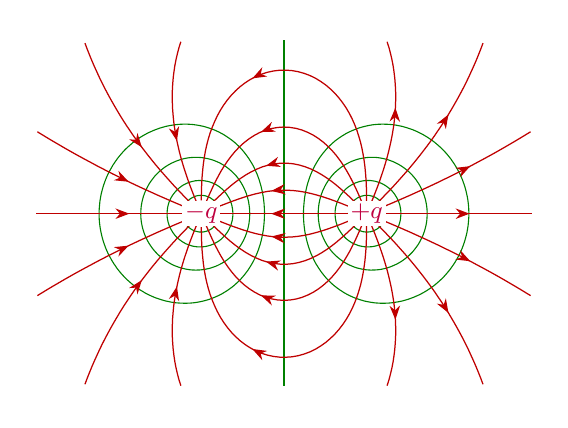
\begin{tikzpicture}[scale=1.05]
\clip (-3.1,-2.25) rectangle (3.1,2.25);
\draw[green!50!black,thin] plot coordinates {(-1.072,-0.211) (-1.096,-0.202) (-1.120,-0.189) (-1.150,-0.167) (-1.172,-0.144) (-1.193,-0.115) (-1.211,-0.078) (-1.218,-0.056) (-1.225,-0.011) (-1.223,0.033) (-1.217,0.058) (-1.201,0.100) (-1.188,0.122) (-1.169,0.148) (-1.145,0.171) (-1.120,0.189) (-1.072,0.211) (-1.048,0.218) (-1.000,0.223) (-0.952,0.217) (-0.928,0.209) (-0.886,0.189) (-0.856,0.167) (-0.834,0.144) (-0.817,0.122) (-0.804,0.100) (-0.787,0.056) (-0.783,0.032) (-0.781,-0.011) (-0.783,-0.033) (-0.794,-0.078) (-0.807,-0.105) (-0.831,-0.141) (-0.855,-0.166) (-0.880,-0.185) (-0.904,-0.199) (-0.933,-0.211) (-0.976,-0.221) (-1.024,-0.222) (-1.072,-0.211)};
\draw[green!50!black,thin] plot coordinates {(-1.096,-0.394) (-1.120,-0.388) (-1.169,-0.371) (-1.193,-0.360) (-1.221,-0.344) (-1.253,-0.322) (-1.281,-0.300) (-1.304,-0.278) (-1.323,-0.256) (-1.340,-0.233) (-1.361,-0.199) (-1.378,-0.167) (-1.388,-0.144) (-1.402,-0.100) (-1.410,-0.060) (-1.413,-0.033) (-1.414,0.011) (-1.410,0.056) (-1.407,0.078) (-1.396,0.122) (-1.386,0.149) (-1.368,0.189) (-1.355,0.211) (-1.337,0.237) (-1.313,0.267) (-1.289,0.292) (-1.265,0.313) (-1.241,0.331) (-1.217,0.347) (-1.178,0.367) (-1.145,0.380) (-1.115,0.389) (-1.072,0.398) (-1.024,0.402) (-0.976,0.400) (-0.928,0.392) (-0.904,0.386) (-0.855,0.368) (-0.831,0.357) (-0.807,0.343) (-0.777,0.322) (-0.750,0.300) (-0.728,0.278) (-0.708,0.256) (-0.687,0.226) (-0.664,0.189) (-0.653,0.167) (-0.639,0.128) (-0.630,0.100) (-0.622,0.056) (-0.618,0.011) (-0.619,-0.033) (-0.625,-0.078) (-0.637,-0.122) (-0.644,-0.144) (-0.663,-0.185) (-0.677,-0.211) (-0.691,-0.233) (-0.711,-0.259) (-0.735,-0.285) (-0.759,-0.308) (-0.783,-0.327) (-0.810,-0.344) (-0.852,-0.367) (-0.880,-0.378) (-0.915,-0.389) (-0.952,-0.397) (-1.000,-0.402) (-1.048,-0.401) (-1.096,-0.394)};
\draw[green!50!black,thin] plot coordinates {(-1.120,-0.680) (-1.145,-0.677) (-1.193,-0.669) (-1.241,-0.657) (-1.265,-0.650) (-1.311,-0.633) (-1.337,-0.622) (-1.361,-0.610) (-1.400,-0.589) (-1.434,-0.567) (-1.458,-0.550) (-1.482,-0.531) (-1.506,-0.511) (-1.530,-0.488) (-1.554,-0.463) (-1.578,-0.435) (-1.597,-0.411) (-1.612,-0.389) (-1.627,-0.367) (-1.651,-0.326) (-1.664,-0.300) (-1.675,-0.276) (-1.692,-0.233) (-1.699,-0.211) (-1.712,-0.167) (-1.721,-0.122) (-1.725,-0.100) (-1.730,-0.056) (-1.732,-0.011) (-1.731,0.033) (-1.728,0.078) (-1.723,0.112) (-1.717,0.144) (-1.706,0.189) (-1.699,0.212) (-1.683,0.256) (-1.674,0.278) (-1.652,0.322) (-1.640,0.344) (-1.627,0.367) (-1.602,0.403) (-1.579,0.433) (-1.561,0.456) (-1.540,0.478) (-1.518,0.500) (-1.493,0.522) (-1.466,0.544) (-1.435,0.567) (-1.410,0.583) (-1.386,0.597) (-1.360,0.611) (-1.313,0.632) (-1.289,0.642) (-1.247,0.656) (-1.217,0.664) (-1.169,0.674) (-1.137,0.678) (-1.096,0.681) (-1.048,0.682) (-1.000,0.679) (-0.976,0.676) (-0.928,0.667) (-0.883,0.656) (-0.855,0.647) (-0.820,0.633) (-0.783,0.617) (-0.759,0.604) (-0.733,0.589) (-0.699,0.567) (-0.669,0.544) (-0.643,0.522) (-0.619,0.500) (-0.597,0.478) (-0.577,0.456) (-0.559,0.433) (-0.542,0.410) (-0.518,0.374) (-0.501,0.344) (-0.489,0.322) (-0.470,0.280) (-0.460,0.256) (-0.446,0.213) (-0.439,0.189) (-0.428,0.144) (-0.422,0.104) (-0.418,0.078) (-0.415,0.033) (-0.414,-0.011) (-0.416,-0.056) (-0.421,-0.100) (-0.424,-0.122) (-0.433,-0.167) (-0.445,-0.211) (-0.452,-0.233) (-0.469,-0.278) (-0.479,-0.300) (-0.494,-0.331) (-0.514,-0.367) (-0.528,-0.389) (-0.543,-0.411) (-0.566,-0.442) (-0.590,-0.471) (-0.614,-0.496) (-0.639,-0.519) (-0.663,-0.539) (-0.687,-0.558) (-0.711,-0.575) (-0.735,-0.590) (-0.773,-0.611) (-0.807,-0.628) (-0.831,-0.638) (-0.880,-0.655) (-0.904,-0.662) (-0.952,-0.672) (-0.993,-0.678) (-1.024,-0.681) (-1.072,-0.682) (-1.120,-0.680)};
\draw[green!50!black,thin] plot coordinates {(-1.289,-1.079) (-1.313,-1.077) (-1.361,-1.070) (-1.410,-1.060) (-1.434,-1.055) (-1.482,-1.041) (-1.507,-1.033) (-1.554,-1.017) (-1.578,-1.007) (-1.619,-0.989) (-1.651,-0.973) (-1.675,-0.961) (-1.703,-0.944) (-1.740,-0.922) (-1.771,-0.901) (-1.795,-0.884) (-1.819,-0.866) (-1.843,-0.846) (-1.867,-0.825) (-1.892,-0.803) (-1.916,-0.780) (-1.940,-0.755) (-1.964,-0.729) (-1.988,-0.700) (-2.006,-0.678) (-2.023,-0.656) (-2.038,-0.633) (-2.060,-0.601) (-2.081,-0.567) (-2.094,-0.544) (-2.108,-0.518) (-2.129,-0.478) (-2.139,-0.456) (-2.157,-0.414) (-2.166,-0.389) (-2.181,-0.347) (-2.189,-0.322) (-2.201,-0.278) (-2.206,-0.256) (-2.216,-0.211) (-2.224,-0.167) (-2.229,-0.126) (-2.232,-0.100) (-2.235,-0.056) (-2.236,-0.011) (-2.236,0.033) (-2.233,0.078) (-2.229,0.122) (-2.227,0.144) (-2.220,0.189) (-2.212,0.233) (-2.205,0.262) (-2.195,0.300) (-2.182,0.344) (-2.174,0.367) (-2.158,0.411) (-2.149,0.433) (-2.133,0.469) (-2.118,0.500) (-2.106,0.522) (-2.084,0.561) (-2.068,0.589) (-2.053,0.611) (-2.036,0.636) (-2.012,0.670) (-1.988,0.700) (-1.969,0.722) (-1.950,0.744) (-1.929,0.767) (-1.907,0.789) (-1.883,0.811) (-1.858,0.833) (-1.832,0.856) (-1.803,0.878) (-1.773,0.900) (-1.747,0.917) (-1.723,0.933) (-1.699,0.947) (-1.663,0.967) (-1.627,0.985) (-1.602,0.996) (-1.568,1.011) (-1.530,1.025) (-1.506,1.034) (-1.458,1.048) (-1.429,1.056) (-1.386,1.065) (-1.337,1.073) (-1.301,1.078) (-1.265,1.081) (-1.217,1.083) (-1.169,1.083) (-1.120,1.080) (-1.096,1.078) (-1.048,1.071) (-1.000,1.062) (-0.972,1.056) (-0.928,1.043) (-0.897,1.033) (-0.855,1.018) (-0.831,1.008) (-0.790,0.989) (-0.759,0.973) (-0.735,0.960) (-0.710,0.944) (-0.676,0.922) (-0.645,0.900) (-0.616,0.878) (-0.590,0.856) (-0.566,0.834) (-0.542,0.811) (-0.521,0.789) (-0.501,0.767) (-0.482,0.744) (-0.465,0.722) (-0.446,0.697) (-0.422,0.662) (-0.404,0.633) (-0.390,0.611) (-0.373,0.581) (-0.355,0.544) (-0.345,0.522) (-0.325,0.478) (-0.317,0.456) (-0.301,0.412) (-0.294,0.389) (-0.281,0.344) (-0.275,0.322) (-0.265,0.278) (-0.256,0.233) (-0.252,0.211) (-0.246,0.167) (-0.241,0.122) (-0.238,0.078) (-0.236,0.033) (-0.236,-0.011) (-0.237,-0.056) (-0.240,-0.100) (-0.244,-0.144) (-0.249,-0.189) (-0.253,-0.215) (-0.260,-0.256) (-0.270,-0.300) (-0.277,-0.331) (-0.287,-0.367) (-0.301,-0.411) (-0.308,-0.433) (-0.325,-0.477) (-0.335,-0.500) (-0.349,-0.533) (-0.366,-0.567) (-0.378,-0.589) (-0.398,-0.624) (-0.418,-0.656) (-0.432,-0.678) (-0.448,-0.700) (-0.470,-0.729) (-0.494,-0.758) (-0.518,-0.786) (-0.542,-0.811) (-0.565,-0.833) (-0.590,-0.856) (-0.614,-0.877) (-0.639,-0.896) (-0.663,-0.913) (-0.687,-0.930) (-0.711,-0.945) (-0.747,-0.967) (-0.783,-0.986) (-0.807,-0.997) (-0.839,-1.011) (-0.880,-1.027) (-0.904,-1.036) (-0.952,-1.050) (-0.976,-1.056) (-1.024,-1.067) (-1.072,-1.075) (-1.098,-1.078) (-1.145,-1.082) (-1.193,-1.083) (-1.241,-1.082) (-1.289,-1.079)};
\draw[green!50!black,thin] plot coordinates {(0.000,2.100) (-0.000,2.056) (-0.000,2.011) (0.000,1.967) (-0.000,1.922) (0.000,1.878) (-0.000,1.833) (0.000,1.789) (-0.000,1.744) (0.000,1.700) (0.000,1.656) (0.000,1.611) (-0.000,1.567) (0.000,1.522) (0.000,1.478) (0.000,1.433) (0.000,1.389) (-0.000,1.344) (-0.000,1.300) (-0.000,1.256) (-0.000,1.211) (-0.000,1.167) (-0.000,1.122) (0.000,1.078) (0.000,1.033) (-0.000,0.989) (0.000,0.944) (-0.000,0.900) (-0.000,0.856) (0.000,0.811) (-0.000,0.767) (-0.000,0.722) (0.000,0.678) (-0.000,0.633) (0.000,0.589) (-0.000,0.544) (0.000,0.500) (0.000,0.456) (0.000,0.411) (-0.000,0.367) (-0.000,0.322) (0.000,0.278) (0.000,0.233) (-0.000,0.189) (-0.000,0.144) (0.000,0.100) (0.000,0.056) (0.000,0.011) (0.000,-0.033) (-0.000,-0.078) (-0.000,-0.122) (0.000,-0.167) (-0.000,-0.211) (-0.000,-0.256) (0.000,-0.300) (-0.000,-0.344) (0.000,-0.389) (0.000,-0.433) (-0.000,-0.478) (-0.000,-0.522) (0.000,-0.567) (-0.000,-0.611) (-0.000,-0.656) (-0.000,-0.700) (-0.000,-0.744) (-0.000,-0.789) (-0.000,-0.833) (-0.000,-0.878) (0.000,-0.922) (-0.000,-0.967) (0.000,-1.011) (0.000,-1.056) (-0.000,-1.100) (0.000,-1.144) (-0.000,-1.189) (0.000,-1.233) (-0.000,-1.278) (0.000,-1.322) (0.000,-1.367) (-0.000,-1.411) (0.000,-1.456) (0.000,-1.500) (0.000,-1.544) (0.000,-1.589) (-0.000,-1.633) (-0.000,-1.678) (-0.000,-1.722) (-0.000,-1.767) (-0.000,-1.811) (-0.000,-1.856) (0.000,-1.900) (0.000,-1.944) (-0.000,-1.989) (0.000,-2.033) (-0.000,-2.078)};
\draw[green!50!black,thin] plot coordinates {(1.120,-1.080) (1.169,-1.083) (1.217,-1.083) (1.265,-1.081) (1.301,-1.078) (1.337,-1.073) (1.386,-1.065) (1.429,-1.056) (1.458,-1.048) (1.506,-1.034) (1.530,-1.025) (1.568,-1.011) (1.602,-0.996) (1.627,-0.985) (1.663,-0.967) (1.699,-0.947) (1.723,-0.933) (1.747,-0.917) (1.773,-0.900) (1.803,-0.878) (1.832,-0.856) (1.858,-0.833) (1.883,-0.811) (1.907,-0.789) (1.929,-0.767) (1.950,-0.744) (1.969,-0.722) (1.988,-0.700) (2.012,-0.670) (2.036,-0.636) (2.053,-0.611) (2.068,-0.589) (2.084,-0.561) (2.106,-0.522) (2.118,-0.500) (2.133,-0.469) (2.149,-0.433) (2.158,-0.411) (2.174,-0.367) (2.182,-0.344) (2.195,-0.300) (2.205,-0.262) (2.212,-0.233) (2.220,-0.189) (2.227,-0.144) (2.229,-0.122) (2.233,-0.078) (2.236,-0.033) (2.236,0.011) (2.235,0.056) (2.232,0.100) (2.229,0.126) (2.224,0.167) (2.216,0.211) (2.206,0.256) (2.201,0.278) (2.189,0.322) (2.181,0.347) (2.166,0.389) (2.157,0.414) (2.139,0.456) (2.129,0.478) (2.108,0.518) (2.094,0.544) (2.081,0.567) (2.060,0.601) (2.038,0.633) (2.023,0.656) (2.006,0.678) (1.988,0.700) (1.964,0.729) (1.940,0.755) (1.916,0.780) (1.892,0.803) (1.867,0.825) (1.843,0.846) (1.819,0.866) (1.795,0.884) (1.771,0.901) (1.740,0.922) (1.703,0.944) (1.675,0.961) (1.651,0.973) (1.619,0.989) (1.578,1.007) (1.554,1.017) (1.507,1.033) (1.482,1.041) (1.434,1.055) (1.410,1.060) (1.361,1.070) (1.313,1.077) (1.289,1.079) (1.241,1.082) (1.193,1.083) (1.145,1.082) (1.098,1.078) (1.072,1.075) (1.024,1.067) (0.976,1.056) (0.952,1.050) (0.904,1.036) (0.880,1.027) (0.839,1.011) (0.807,0.997) (0.783,0.986) (0.747,0.967) (0.711,0.945) (0.687,0.930) (0.663,0.913) (0.639,0.896) (0.614,0.877) (0.590,0.856) (0.565,0.833) (0.542,0.811) (0.518,0.786) (0.494,0.758) (0.470,0.729) (0.448,0.700) (0.432,0.678) (0.418,0.656) (0.398,0.624) (0.378,0.589) (0.366,0.567) (0.349,0.533) (0.335,0.500) (0.325,0.477) (0.308,0.433) (0.301,0.411) (0.287,0.367) (0.277,0.331) (0.270,0.300) (0.260,0.256) (0.253,0.215) (0.249,0.189) (0.244,0.144) (0.240,0.100) (0.237,0.056) (0.236,0.011) (0.236,-0.033) (0.238,-0.078) (0.241,-0.122) (0.246,-0.167) (0.252,-0.211) (0.256,-0.233) (0.265,-0.278) (0.275,-0.322) (0.281,-0.344) (0.294,-0.389) (0.301,-0.412) (0.317,-0.456) (0.325,-0.478) (0.345,-0.522) (0.355,-0.544) (0.373,-0.581) (0.390,-0.611) (0.404,-0.633) (0.422,-0.662) (0.446,-0.697) (0.465,-0.722) (0.482,-0.744) (0.501,-0.767) (0.521,-0.789) (0.542,-0.811) (0.566,-0.834) (0.590,-0.856) (0.616,-0.878) (0.645,-0.900) (0.676,-0.922) (0.710,-0.944) (0.735,-0.960) (0.759,-0.973) (0.790,-0.989) (0.831,-1.008) (0.855,-1.018) (0.897,-1.033) (0.928,-1.043) (0.972,-1.056) (1.000,-1.062) (1.048,-1.071) (1.096,-1.078) (1.120,-1.080)};
\draw[green!50!black,thin] plot coordinates {(1.000,-0.679) (1.048,-0.682) (1.096,-0.681) (1.137,-0.678) (1.169,-0.674) (1.217,-0.664) (1.247,-0.656) (1.289,-0.642) (1.313,-0.632) (1.360,-0.611) (1.386,-0.597) (1.410,-0.583) (1.435,-0.567) (1.466,-0.544) (1.493,-0.522) (1.518,-0.500) (1.540,-0.478) (1.561,-0.456) (1.579,-0.433) (1.602,-0.403) (1.627,-0.367) (1.640,-0.344) (1.652,-0.322) (1.674,-0.278) (1.683,-0.256) (1.699,-0.212) (1.706,-0.189) (1.717,-0.144) (1.723,-0.112) (1.728,-0.078) (1.731,-0.033) (1.732,0.011) (1.730,0.056) (1.725,0.100) (1.721,0.122) (1.712,0.167) (1.699,0.211) (1.692,0.233) (1.675,0.276) (1.664,0.300) (1.651,0.326) (1.627,0.367) (1.612,0.389) (1.597,0.411) (1.578,0.435) (1.554,0.463) (1.530,0.488) (1.506,0.511) (1.482,0.531) (1.458,0.550) (1.434,0.567) (1.400,0.589) (1.361,0.610) (1.337,0.622) (1.311,0.633) (1.265,0.650) (1.241,0.657) (1.193,0.669) (1.145,0.677) (1.120,0.680) (1.072,0.682) (1.024,0.681) (0.993,0.678) (0.952,0.672) (0.904,0.662) (0.880,0.655) (0.831,0.638) (0.807,0.628) (0.773,0.611) (0.735,0.590) (0.711,0.575) (0.687,0.558) (0.663,0.539) (0.639,0.519) (0.614,0.496) (0.590,0.471) (0.566,0.442) (0.543,0.411) (0.528,0.389) (0.514,0.367) (0.494,0.331) (0.479,0.300) (0.469,0.278) (0.452,0.233) (0.445,0.211) (0.433,0.167) (0.424,0.122) (0.421,0.100) (0.416,0.056) (0.414,0.011) (0.415,-0.033) (0.418,-0.078) (0.422,-0.104) (0.428,-0.144) (0.439,-0.189) (0.446,-0.213) (0.460,-0.256) (0.470,-0.280) (0.489,-0.322) (0.501,-0.344) (0.518,-0.374) (0.542,-0.410) (0.559,-0.433) (0.577,-0.456) (0.597,-0.478) (0.619,-0.500) (0.643,-0.522) (0.669,-0.544) (0.699,-0.567) (0.733,-0.589) (0.759,-0.604) (0.783,-0.617) (0.820,-0.633) (0.855,-0.647) (0.883,-0.656) (0.928,-0.667) (0.976,-0.676) (1.000,-0.679)};
\draw[green!50!black,thin] plot coordinates {(0.928,-0.392) (0.976,-0.400) (1.024,-0.402) (1.072,-0.398) (1.115,-0.389) (1.145,-0.380) (1.178,-0.367) (1.217,-0.347) (1.241,-0.331) (1.265,-0.313) (1.289,-0.292) (1.313,-0.267) (1.337,-0.237) (1.355,-0.211) (1.368,-0.189) (1.386,-0.149) (1.396,-0.122) (1.407,-0.078) (1.410,-0.056) (1.414,-0.011) (1.413,0.033) (1.410,0.060) (1.402,0.100) (1.388,0.144) (1.378,0.167) (1.361,0.199) (1.340,0.233) (1.323,0.256) (1.304,0.278) (1.281,0.300) (1.253,0.322) (1.221,0.344) (1.193,0.360) (1.169,0.371) (1.120,0.388) (1.096,0.394) (1.048,0.401) (1.000,0.402) (0.952,0.397) (0.915,0.389) (0.880,0.378) (0.852,0.367) (0.810,0.344) (0.783,0.327) (0.759,0.308) (0.735,0.285) (0.711,0.259) (0.691,0.233) (0.677,0.211) (0.663,0.185) (0.644,0.144) (0.637,0.122) (0.625,0.078) (0.619,0.033) (0.618,-0.011) (0.622,-0.056) (0.630,-0.100) (0.639,-0.128) (0.653,-0.167) (0.664,-0.189) (0.687,-0.226) (0.708,-0.256) (0.728,-0.278) (0.750,-0.300) (0.777,-0.322) (0.807,-0.343) (0.831,-0.357) (0.855,-0.368) (0.904,-0.386) (0.928,-0.392)};
\draw[green!50!black,thin] plot coordinates {(0.952,-0.217) (1.000,-0.223) (1.048,-0.218) (1.072,-0.211) (1.120,-0.189) (1.145,-0.171) (1.169,-0.148) (1.188,-0.122) (1.201,-0.100) (1.217,-0.058) (1.223,-0.033) (1.225,0.011) (1.218,0.056) (1.211,0.078) (1.193,0.115) (1.172,0.144) (1.150,0.167) (1.120,0.189) (1.096,0.202) (1.072,0.211) (1.024,0.222) (0.976,0.221) (0.933,0.211) (0.904,0.199) (0.880,0.185) (0.855,0.166) (0.831,0.141) (0.807,0.105) (0.794,0.078) (0.783,0.033) (0.781,0.011) (0.783,-0.032) (0.787,-0.056) (0.804,-0.100) (0.817,-0.122) (0.834,-0.144) (0.856,-0.167) (0.886,-0.189) (0.928,-0.209) (0.952,-0.217)};
\draw[field,line width=.45pt] plot coordinates {(-1.247,2.080) (-1.270,2.009) (-1.289,1.936) (-1.306,1.863) (-1.320,1.790) (-1.331,1.715) (-1.340,1.641) (-1.346,1.566) (-1.350,1.491) (-1.352,1.416) (-1.350,1.341) (-1.347,1.266) (-1.341,1.192) (-1.334,1.117) (-1.324,1.043) (-1.312,0.969) (-1.298,0.895) (-1.282,0.822) (-1.265,0.749) (-1.246,0.676) (-1.225,0.604) (-1.203,0.532) (-1.179,0.461) (-1.155,0.390) (-1.129,0.320) (-1.102,0.250) (-1.074,0.180) (-1.046,0.111)};
\draw[field,line width=.45pt] plot coordinates {(-2.407,2.063) (-2.381,1.993) (-2.353,1.923) (-2.325,1.854) (-2.295,1.785) (-2.264,1.717) (-2.233,1.649) (-2.200,1.581) (-2.166,1.514) (-2.131,1.448) (-2.095,1.382) (-2.058,1.317) (-2.020,1.252) (-1.982,1.188) (-1.942,1.124) (-1.901,1.061) (-1.859,0.999) (-1.817,0.937) (-1.773,0.876) (-1.729,0.816) (-1.683,0.756) (-1.637,0.697) (-1.590,0.638) (-1.543,0.581) (-1.494,0.523) (-1.445,0.467) (-1.395,0.411) (-1.345,0.355) (-1.294,0.300) (-1.242,0.246) (-1.190,0.192) (-1.138,0.138) (-1.085,0.085)};
\draw[field,line width=.45pt] plot coordinates {(-2.983,0.991) (-2.919,0.952) (-2.855,0.913) (-2.791,0.875) (-2.726,0.837) (-2.661,0.799) (-2.596,0.762) (-2.531,0.725) (-2.465,0.689) (-2.399,0.653) (-2.333,0.618) (-2.267,0.582) (-2.201,0.548) (-2.134,0.513) (-2.067,0.479) (-2.000,0.446) (-1.932,0.413) (-1.865,0.380) (-1.797,0.348) (-1.729,0.316) (-1.661,0.285) (-1.593,0.254) (-1.525,0.223) (-1.456,0.193) (-1.387,0.163) (-1.318,0.133) (-1.249,0.104) (-1.180,0.075) (-1.111,0.046)};
\draw[field,line width=.45pt] plot coordinates {(-2.995,0.000) (-2.920,0.000) (-2.845,0.000) (-2.770,0.000) (-2.695,0.000) (-2.620,0.000) (-2.545,0.000) (-2.470,0.000) (-2.395,0.000) (-2.320,0.000) (-2.245,0.000) (-2.170,0.000) (-2.095,0.000) (-2.020,0.000) (-1.945,0.000) (-1.870,0.000) (-1.795,0.000) (-1.720,0.000) (-1.645,0.000) (-1.570,0.000) (-1.495,0.000) (-1.420,0.000) (-1.345,0.000) (-1.270,0.000) (-1.195,0.000) (-1.120,0.000)};
\draw[field,line width=.45pt] plot coordinates {(-2.983,-0.991) (-2.919,-0.952) (-2.855,-0.913) (-2.791,-0.875) (-2.726,-0.837) (-2.661,-0.799) (-2.596,-0.762) (-2.531,-0.725) (-2.465,-0.689) (-2.399,-0.653) (-2.333,-0.618) (-2.267,-0.582) (-2.201,-0.548) (-2.134,-0.513) (-2.067,-0.479) (-2.000,-0.446) (-1.932,-0.413) (-1.865,-0.380) (-1.797,-0.348) (-1.729,-0.316) (-1.661,-0.285) (-1.593,-0.254) (-1.525,-0.223) (-1.456,-0.193) (-1.387,-0.163) (-1.318,-0.133) (-1.249,-0.104) (-1.180,-0.075) (-1.111,-0.046)};
\draw[field,line width=.45pt] plot coordinates {(-2.407,-2.063) (-2.381,-1.993) (-2.353,-1.923) (-2.325,-1.854) (-2.295,-1.785) (-2.264,-1.717) (-2.233,-1.649) (-2.200,-1.581) (-2.166,-1.514) (-2.131,-1.448) (-2.095,-1.382) (-2.058,-1.317) (-2.020,-1.252) (-1.982,-1.188) (-1.942,-1.124) (-1.901,-1.061) (-1.859,-0.999) (-1.817,-0.937) (-1.773,-0.876) (-1.729,-0.816) (-1.683,-0.756) (-1.637,-0.697) (-1.590,-0.638) (-1.543,-0.581) (-1.494,-0.523) (-1.445,-0.467) (-1.395,-0.411) (-1.345,-0.355) (-1.294,-0.300) (-1.242,-0.246) (-1.190,-0.192) (-1.138,-0.138) (-1.085,-0.085)};
\draw[field,line width=.45pt] plot coordinates {(-1.247,-2.080) (-1.270,-2.009) (-1.289,-1.936) (-1.306,-1.863) (-1.320,-1.790) (-1.331,-1.715) (-1.340,-1.641) (-1.346,-1.566) (-1.350,-1.491) (-1.352,-1.416) (-1.350,-1.341) (-1.347,-1.266) (-1.341,-1.192) (-1.334,-1.117) (-1.324,-1.043) (-1.312,-0.969) (-1.298,-0.895) (-1.282,-0.822) (-1.265,-0.749) (-1.246,-0.676) (-1.225,-0.604) (-1.203,-0.532) (-1.179,-0.461) (-1.155,-0.390) (-1.129,-0.320) (-1.102,-0.250) (-1.074,-0.180) (-1.046,-0.111)};
\draw[field,line width=.45pt] plot coordinates {(1.120,0.000) (1.195,0.000) (1.270,0.000) (1.345,0.000) (1.420,0.000) (1.495,0.000) (1.570,0.000) (1.645,0.000) (1.720,0.000) (1.795,0.000) (1.870,0.000) (1.945,0.000) (2.020,0.000) (2.095,0.000) (2.170,0.000) (2.245,0.000) (2.320,0.000) (2.395,0.000) (2.470,0.000) (2.545,0.000) (2.620,0.000) (2.695,0.000) (2.770,0.000) (2.845,0.000) (2.920,0.000) (2.995,0.000)};
\draw[field,line width=.45pt] plot coordinates {(1.111,0.046) (1.180,0.075) (1.249,0.104) (1.318,0.133) (1.387,0.163) (1.456,0.193) (1.525,0.223) (1.593,0.254) (1.661,0.285) (1.729,0.316) (1.797,0.348) (1.865,0.380) (1.932,0.413) (2.000,0.446) (2.067,0.479) (2.134,0.513) (2.201,0.548) (2.267,0.582) (2.333,0.618) (2.399,0.653) (2.465,0.689) (2.531,0.725) (2.596,0.762) (2.661,0.799) (2.726,0.837) (2.791,0.875) (2.855,0.913) (2.919,0.952) (2.983,0.991)};
\draw[field,line width=.45pt] plot coordinates {(1.085,0.085) (1.138,0.138) (1.190,0.192) (1.242,0.246) (1.294,0.300) (1.345,0.355) (1.395,0.411) (1.445,0.467) (1.494,0.523) (1.543,0.581) (1.590,0.638) (1.637,0.697) (1.683,0.756) (1.729,0.816) (1.773,0.876) (1.817,0.937) (1.859,0.999) (1.901,1.061) (1.942,1.124) (1.982,1.188) (2.020,1.252) (2.058,1.317) (2.095,1.382) (2.131,1.448) (2.166,1.514) (2.200,1.581) (2.233,1.649) (2.264,1.717) (2.295,1.785) (2.325,1.854) (2.353,1.923) (2.381,1.993) (2.407,2.063)};
\draw[field,line width=.45pt] plot coordinates {(1.046,0.111) (1.074,0.180) (1.102,0.250) (1.129,0.320) (1.155,0.390) (1.179,0.461) (1.203,0.532) (1.225,0.604) (1.246,0.676) (1.265,0.749) (1.282,0.822) (1.298,0.895) (1.312,0.969) (1.324,1.043) (1.334,1.117) (1.341,1.192) (1.347,1.266) (1.350,1.341) (1.352,1.416) (1.350,1.491) (1.346,1.566) (1.340,1.641) (1.331,1.715) (1.320,1.790) (1.306,1.863) (1.289,1.936) (1.270,2.009) (1.247,2.080)};
\draw[field,line width=.45pt] plot coordinates {(1.000,0.120) (0.999,0.195) (0.998,0.270) (0.996,0.345) (0.992,0.420) (0.986,0.495) (0.979,0.569) (0.969,0.644) (0.957,0.718) (0.943,0.791) (0.926,0.864) (0.905,0.936) (0.882,1.008) (0.855,1.078) (0.825,1.146) (0.791,1.213) (0.753,1.278) (0.711,1.340) (0.665,1.400) (0.616,1.456) (0.562,1.508) (0.505,1.557) (0.444,1.600) (0.380,1.639) (0.312,1.672) (0.242,1.698) (0.170,1.718) (0.096,1.731) (0.021,1.736) (-0.054,1.735) (-0.128,1.726) (-0.202,1.710) (-0.273,1.687) (-0.342,1.658) (-0.408,1.623) (-0.471,1.582) (-0.531,1.536) (-0.586,1.486) (-0.638,1.432) (-0.686,1.374) (-0.730,1.313) (-0.770,1.250) (-0.806,1.184) (-0.838,1.116) (-0.867,1.047) (-0.893,0.977) (-0.915,0.905) (-0.934,0.832) (-0.950,0.759) (-0.963,0.685) (-0.974,0.611) (-0.982,0.537) (-0.989,0.462) (-0.994,0.387) (-0.997,0.312) (-0.999,0.237) (-1.000,0.162)};
\draw[field,line width=.45pt] plot coordinates {(0.954,0.111) (0.925,0.180) (0.895,0.249) (0.864,0.317) (0.831,0.384) (0.797,0.451) (0.760,0.516) (0.721,0.580) (0.679,0.643) (0.634,0.703) (0.585,0.760) (0.533,0.814) (0.477,0.864) (0.418,0.909) (0.355,0.950) (0.288,0.984) (0.218,1.012) (0.146,1.032) (0.072,1.044) (-0.003,1.048) (-0.078,1.043) (-0.151,1.030) (-0.224,1.010) (-0.293,0.982) (-0.359,0.947) (-0.422,0.906) (-0.482,0.860) (-0.537,0.810) (-0.589,0.756) (-0.637,0.698) (-0.682,0.638) (-0.724,0.576) (-0.763,0.512) (-0.799,0.446) (-0.834,0.379) (-0.866,0.312) (-0.897,0.244) (-0.927,0.175) (-0.956,0.106)};
\draw[field,line width=.45pt] plot coordinates {(0.915,0.085) (0.862,0.138) (0.808,0.190) (0.753,0.241) (0.697,0.291) (0.640,0.340) (0.582,0.386) (0.521,0.430) (0.458,0.471) (0.393,0.508) (0.325,0.541) (0.255,0.568) (0.184,0.589) (0.110,0.604) (0.035,0.611) (-0.040,0.611) (-0.114,0.603) (-0.188,0.588) (-0.260,0.567) (-0.329,0.539) (-0.397,0.506) (-0.462,0.469) (-0.524,0.428) (-0.585,0.384) (-0.644,0.337) (-0.701,0.288) (-0.756,0.238) (-0.811,0.187) (-0.865,0.135) (-0.918,0.082)};
\draw[field,line width=.45pt] plot coordinates {(0.889,0.046) (0.820,0.074) (0.750,0.102) (0.680,0.130) (0.610,0.156) (0.540,0.181) (0.468,0.205) (0.396,0.226) (0.324,0.245) (0.250,0.261) (0.176,0.273) (0.102,0.281) (0.027,0.284) (-0.048,0.284) (-0.123,0.279) (-0.197,0.270) (-0.271,0.256) (-0.344,0.240) (-0.417,0.220) (-0.488,0.198) (-0.559,0.174) (-0.630,0.149) (-0.700,0.122) (-0.770,0.095) (-0.839,0.066)};
\draw[field,line width=.45pt] plot coordinates {(0.880,0.000) (0.805,0.000) (0.730,0.000) (0.655,0.000) (0.580,0.000) (0.505,0.000) (0.430,0.000) (0.355,0.000) (0.280,0.000) (0.205,0.000) (0.130,0.000) (0.055,0.000) (-0.020,0.000) (-0.095,0.000) (-0.170,0.000) (-0.245,0.000) (-0.320,0.000) (-0.395,0.000) (-0.470,0.000) (-0.545,0.000) (-0.620,0.000) (-0.695,0.000) (-0.770,0.000) (-0.845,0.000)};
\draw[field,line width=.45pt] plot coordinates {(0.889,-0.046) (0.820,-0.074) (0.750,-0.102) (0.680,-0.130) (0.610,-0.156) (0.540,-0.181) (0.468,-0.205) (0.396,-0.226) (0.324,-0.245) (0.250,-0.261) (0.176,-0.273) (0.102,-0.281) (0.027,-0.284) (-0.048,-0.284) (-0.123,-0.279) (-0.197,-0.270) (-0.271,-0.256) (-0.344,-0.240) (-0.417,-0.220) (-0.488,-0.198) (-0.559,-0.174) (-0.630,-0.149) (-0.700,-0.122) (-0.770,-0.095) (-0.839,-0.066)};
\draw[field,line width=.45pt] plot coordinates {(0.915,-0.085) (0.862,-0.138) (0.808,-0.190) (0.753,-0.241) (0.697,-0.291) (0.640,-0.340) (0.582,-0.386) (0.521,-0.430) (0.458,-0.471) (0.393,-0.508) (0.325,-0.541) (0.255,-0.568) (0.184,-0.589) (0.110,-0.604) (0.035,-0.611) (-0.040,-0.611) (-0.114,-0.603) (-0.188,-0.588) (-0.260,-0.567) (-0.329,-0.539) (-0.397,-0.506) (-0.462,-0.469) (-0.524,-0.428) (-0.585,-0.384) (-0.644,-0.337) (-0.701,-0.288) (-0.756,-0.238) (-0.811,-0.187) (-0.865,-0.135) (-0.918,-0.082)};
\draw[field,line width=.45pt] plot coordinates {(0.954,-0.111) (0.925,-0.180) (0.895,-0.249) (0.864,-0.317) (0.831,-0.384) (0.797,-0.451) (0.760,-0.516) (0.721,-0.580) (0.679,-0.643) (0.634,-0.703) (0.585,-0.760) (0.533,-0.814) (0.477,-0.864) (0.418,-0.909) (0.355,-0.950) (0.288,-0.984) (0.218,-1.012) (0.146,-1.032) (0.072,-1.044) (-0.003,-1.048) (-0.078,-1.043) (-0.151,-1.030) (-0.224,-1.010) (-0.293,-0.982) (-0.359,-0.947) (-0.422,-0.906) (-0.482,-0.860) (-0.537,-0.810) (-0.589,-0.756) (-0.637,-0.698) (-0.682,-0.638) (-0.724,-0.576) (-0.763,-0.512) (-0.799,-0.446) (-0.834,-0.379) (-0.866,-0.312) (-0.897,-0.244) (-0.927,-0.175) (-0.956,-0.106)};
\draw[field,line width=.45pt] plot coordinates {(1.000,-0.120) (0.999,-0.195) (0.998,-0.270) (0.996,-0.345) (0.992,-0.420) (0.986,-0.495) (0.979,-0.569) (0.969,-0.644) (0.957,-0.718) (0.943,-0.791) (0.926,-0.864) (0.905,-0.936) (0.882,-1.008) (0.855,-1.078) (0.825,-1.146) (0.791,-1.213) (0.753,-1.278) (0.711,-1.340) (0.665,-1.400) (0.616,-1.456) (0.562,-1.508) (0.505,-1.557) (0.444,-1.600) (0.380,-1.639) (0.312,-1.672) (0.242,-1.698) (0.170,-1.718) (0.096,-1.731) (0.021,-1.736) (-0.054,-1.735) (-0.128,-1.726) (-0.202,-1.710) (-0.273,-1.687) (-0.342,-1.658) (-0.408,-1.623) (-0.471,-1.582) (-0.531,-1.536) (-0.586,-1.486) (-0.638,-1.432) (-0.686,-1.374) (-0.730,-1.313) (-0.770,-1.250) (-0.806,-1.184) (-0.838,-1.116) (-0.867,-1.047) (-0.893,-0.977) (-0.915,-0.905) (-0.934,-0.832) (-0.950,-0.759) (-0.963,-0.685) (-0.974,-0.611) (-0.982,-0.537) (-0.989,-0.462) (-0.994,-0.387) (-0.997,-0.312) (-0.999,-0.237) (-1.000,-0.162)};
\draw[field,line width=.45pt] plot coordinates {(1.046,-0.111) (1.074,-0.180) (1.102,-0.250) (1.129,-0.320) (1.155,-0.390) (1.179,-0.461) (1.203,-0.532) (1.225,-0.604) (1.246,-0.676) (1.265,-0.749) (1.282,-0.822) (1.298,-0.895) (1.312,-0.969) (1.324,-1.043) (1.334,-1.117) (1.341,-1.192) (1.347,-1.266) (1.350,-1.341) (1.352,-1.416) (1.350,-1.491) (1.346,-1.566) (1.340,-1.641) (1.331,-1.715) (1.320,-1.790) (1.306,-1.863) (1.289,-1.936) (1.270,-2.009) (1.247,-2.080)};
\draw[field,line width=.45pt] plot coordinates {(1.085,-0.085) (1.138,-0.138) (1.190,-0.192) (1.242,-0.246) (1.294,-0.300) (1.345,-0.355) (1.395,-0.411) (1.445,-0.467) (1.494,-0.523) (1.543,-0.581) (1.590,-0.638) (1.637,-0.697) (1.683,-0.756) (1.729,-0.816) (1.773,-0.876) (1.817,-0.937) (1.859,-0.999) (1.901,-1.061) (1.942,-1.124) (1.982,-1.188) (2.020,-1.252) (2.058,-1.317) (2.095,-1.382) (2.131,-1.448) (2.166,-1.514) (2.200,-1.581) (2.233,-1.649) (2.264,-1.717) (2.295,-1.785) (2.325,-1.854) (2.353,-1.923) (2.381,-1.993) (2.407,-2.063)};
\draw[field,line width=.45pt] plot coordinates {(1.111,-0.046) (1.180,-0.075) (1.249,-0.104) (1.318,-0.133) (1.387,-0.163) (1.456,-0.193) (1.525,-0.223) (1.593,-0.254) (1.661,-0.285) (1.729,-0.316) (1.797,-0.348) (1.865,-0.380) (1.932,-0.413) (2.000,-0.446) (2.067,-0.479) (2.134,-0.513) (2.201,-0.548) (2.267,-0.582) (2.333,-0.618) (2.399,-0.653) (2.465,-0.689) (2.531,-0.725) (2.596,-0.762) (2.661,-0.799) (2.726,-0.837) (2.791,-0.875) (2.855,-0.913) (2.919,-0.952) (2.983,-0.991)};
\fill[white](-1,0)circle(.13);
\node[fill=white,inner sep=1pt,text=purple]at(-1,0){$-q$};
\fill[white](1,0)circle(.13);
\node[fill=white,inner sep=1pt,text=purple]at(1,0){$+q$};
\end{tikzpicture}}
Près de $+q$, les lignes de champ divergent ; près de $-q$, elles convergent. Le champ loin des charges sera étudié plus tard.
Tout plan contenant les deux charges est un plan de symétrie : le champ y est contenu. Le plan perpendiculaire à l'axe des charges, situé entre elles, est un plan d'antisymétrie.
\Needspace{65mm}\titr{Quatre charges identiques $q$}
\fig{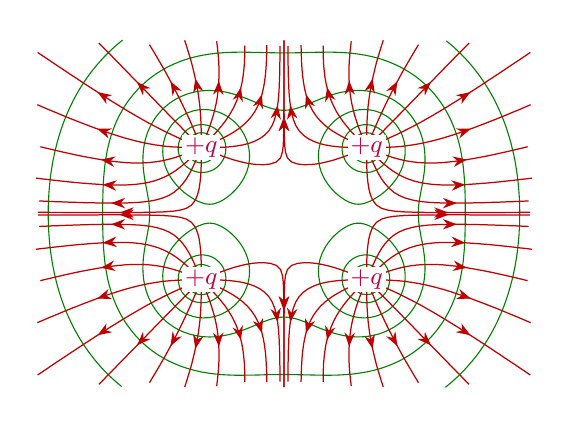
\begin{tikzpicture}[scale=1.05]
\clip (-3.1,-2.25) rectangle (3.1,2.25);
\draw[green!50!black,thin] plot coordinates {(1.952,-2.100) (1.979,-2.078) (2.006,-2.056) (2.032,-2.033) (2.057,-2.011) (2.081,-1.989) (2.105,-1.967) (2.128,-1.944) (2.150,-1.922) (2.172,-1.900) (2.193,-1.878) (2.213,-1.856) (2.233,-1.833) (2.253,-1.810) (2.277,-1.782) (2.301,-1.752) (2.325,-1.722) (2.342,-1.700) (2.358,-1.678) (2.374,-1.656) (2.398,-1.622) (2.420,-1.589) (2.435,-1.567) (2.449,-1.544) (2.470,-1.510) (2.489,-1.478) (2.502,-1.456) (2.518,-1.427) (2.538,-1.389) (2.550,-1.367) (2.566,-1.334) (2.583,-1.300) (2.593,-1.278) (2.613,-1.233) (2.623,-1.211) (2.639,-1.173) (2.650,-1.144) (2.663,-1.111) (2.675,-1.078) (2.687,-1.045) (2.698,-1.011) (2.711,-0.972) (2.719,-0.944) (2.732,-0.900) (2.739,-0.878) (2.750,-0.833) (2.759,-0.799) (2.767,-0.767) (2.777,-0.722) (2.783,-0.692) (2.791,-0.656) (2.799,-0.611) (2.806,-0.567) (2.810,-0.544) (2.817,-0.500) (2.823,-0.456) (2.828,-0.411) (2.831,-0.382) (2.835,-0.344) (2.839,-0.300) (2.843,-0.256) (2.845,-0.211) (2.848,-0.167) (2.850,-0.122) (2.851,-0.078) (2.851,-0.033) (2.852,0.011) (2.851,0.056) (2.850,0.100) (2.849,0.144) (2.847,0.189) (2.844,0.233) (2.841,0.278) (2.837,0.322) (2.833,0.367) (2.831,0.389) (2.826,0.433) (2.820,0.478) (2.813,0.522) (2.807,0.561) (2.803,0.589) (2.795,0.633) (2.786,0.678) (2.782,0.700) (2.772,0.744) (2.761,0.789) (2.756,0.811) (2.745,0.856) (2.735,0.891) (2.726,0.922) (2.712,0.967) (2.705,0.989) (2.691,1.033) (2.683,1.056) (2.667,1.100) (2.659,1.122) (2.641,1.167) (2.632,1.189) (2.614,1.230) (2.603,1.256) (2.590,1.284) (2.572,1.322) (2.561,1.344) (2.542,1.382) (2.527,1.411) (2.514,1.433) (2.494,1.469) (2.476,1.500) (2.463,1.522) (2.446,1.549) (2.422,1.587) (2.405,1.611) (2.390,1.633) (2.373,1.657) (2.349,1.690) (2.325,1.721) (2.307,1.744) (2.290,1.767) (2.271,1.789) (2.252,1.811) (2.229,1.838) (2.205,1.865) (2.181,1.890) (2.157,1.915) (2.133,1.940) (2.108,1.963) (2.084,1.986) (2.060,2.008) (2.036,2.030) (2.012,2.050) (1.988,2.071) (1.964,2.090)};
\draw[green!50!black,thin] plot coordinates {(-1.952,2.100) (-1.979,2.078) (-2.006,2.056) (-2.032,2.033) (-2.057,2.011) (-2.081,1.989) (-2.105,1.967) (-2.128,1.944) (-2.150,1.922) (-2.172,1.900) (-2.193,1.878) (-2.213,1.856) (-2.233,1.833) (-2.253,1.810) (-2.277,1.782) (-2.301,1.752) (-2.325,1.722) (-2.342,1.700) (-2.358,1.678) (-2.374,1.656) (-2.398,1.622) (-2.420,1.589) (-2.435,1.567) (-2.449,1.544) (-2.470,1.510) (-2.489,1.478) (-2.502,1.456) (-2.518,1.427) (-2.538,1.389) (-2.550,1.367) (-2.566,1.334) (-2.583,1.300) (-2.593,1.278) (-2.613,1.233) (-2.623,1.211) (-2.639,1.173) (-2.650,1.144) (-2.663,1.111) (-2.675,1.078) (-2.687,1.045) (-2.698,1.011) (-2.711,0.972) (-2.719,0.944) (-2.732,0.900) (-2.739,0.878) (-2.750,0.833) (-2.759,0.799) (-2.767,0.767) (-2.777,0.722) (-2.783,0.692) (-2.791,0.656) (-2.799,0.611) (-2.806,0.567) (-2.810,0.544) (-2.817,0.500) (-2.823,0.456) (-2.828,0.411) (-2.831,0.382) (-2.835,0.344) (-2.839,0.300) (-2.843,0.256) (-2.845,0.211) (-2.848,0.167) (-2.850,0.122) (-2.851,0.078) (-2.851,0.033) (-2.852,-0.011) (-2.851,-0.056) (-2.850,-0.100) (-2.849,-0.144) (-2.847,-0.189) (-2.844,-0.233) (-2.841,-0.278) (-2.837,-0.322) (-2.833,-0.367) (-2.831,-0.389) (-2.826,-0.433) (-2.820,-0.478) (-2.813,-0.522) (-2.807,-0.561) (-2.803,-0.589) (-2.795,-0.633) (-2.786,-0.678) (-2.782,-0.700) (-2.772,-0.744) (-2.761,-0.789) (-2.756,-0.811) (-2.745,-0.856) (-2.735,-0.891) (-2.726,-0.922) (-2.712,-0.967) (-2.705,-0.989) (-2.691,-1.033) (-2.683,-1.056) (-2.667,-1.100) (-2.659,-1.122) (-2.641,-1.167) (-2.632,-1.189) (-2.614,-1.230) (-2.603,-1.256) (-2.590,-1.284) (-2.572,-1.322) (-2.561,-1.344) (-2.542,-1.382) (-2.527,-1.411) (-2.514,-1.433) (-2.494,-1.469) (-2.476,-1.500) (-2.463,-1.522) (-2.446,-1.549) (-2.422,-1.587) (-2.405,-1.611) (-2.390,-1.633) (-2.373,-1.657) (-2.349,-1.690) (-2.325,-1.721) (-2.307,-1.744) (-2.290,-1.767) (-2.271,-1.789) (-2.252,-1.811) (-2.229,-1.838) (-2.205,-1.865) (-2.181,-1.890) (-2.157,-1.915) (-2.133,-1.940) (-2.108,-1.963) (-2.084,-1.986) (-2.060,-2.008) (-2.036,-2.030) (-2.012,-2.050) (-1.988,-2.071) (-1.964,-2.090)};
\draw[green!50!black,thin] plot coordinates {(-0.759,-1.946) (-0.711,-1.949) (-0.663,-1.951) (-0.614,-1.953) (-0.566,-1.954) (-0.518,-1.954) (-0.470,-1.953) (-0.422,-1.953) (-0.373,-1.952) (-0.325,-1.951) (-0.277,-1.950) (-0.229,-1.948) (-0.181,-1.947) (-0.133,-1.946) (-0.084,-1.946) (-0.036,-1.945) (0.012,-1.945) (0.060,-1.945) (0.108,-1.946) (0.157,-1.947) (0.205,-1.948) (0.253,-1.949) (0.301,-1.950) (0.349,-1.951) (0.398,-1.952) (0.446,-1.953) (0.494,-1.954) (0.542,-1.954) (0.590,-1.953) (0.639,-1.952) (0.687,-1.950) (0.735,-1.947) (0.774,-1.944) (0.807,-1.942) (0.855,-1.936) (0.904,-1.930) (0.952,-1.922) (0.976,-1.918) (1.024,-1.909) (1.062,-1.900) (1.096,-1.892) (1.145,-1.878) (1.169,-1.871) (1.216,-1.856) (1.241,-1.847) (1.276,-1.833) (1.313,-1.818) (1.337,-1.808) (1.377,-1.789) (1.410,-1.773) (1.434,-1.760) (1.461,-1.744) (1.498,-1.722) (1.530,-1.702) (1.554,-1.686) (1.578,-1.669) (1.602,-1.651) (1.627,-1.633) (1.653,-1.611) (1.679,-1.589) (1.704,-1.567) (1.727,-1.544) (1.750,-1.522) (1.771,-1.500) (1.795,-1.474) (1.819,-1.446) (1.843,-1.416) (1.865,-1.389) (1.881,-1.367) (1.897,-1.344) (1.916,-1.317) (1.940,-1.279) (1.954,-1.256) (1.966,-1.233) (1.988,-1.194) (2.002,-1.167) (2.012,-1.144) (2.033,-1.100) (2.042,-1.078) (2.060,-1.033) (2.068,-1.011) (2.083,-0.967) (2.091,-0.944) (2.104,-0.900) (2.110,-0.878) (2.122,-0.833) (2.132,-0.789) (2.137,-0.767) (2.145,-0.722) (2.153,-0.678) (2.157,-0.655) (2.163,-0.611) (2.169,-0.567) (2.173,-0.522) (2.177,-0.478) (2.181,-0.433) (2.182,-0.411) (2.185,-0.367) (2.187,-0.322) (2.189,-0.278) (2.190,-0.233) (2.191,-0.189) (2.192,-0.144) (2.193,-0.100) (2.193,-0.056) (2.193,-0.011) (2.193,0.033) (2.193,0.078) (2.192,0.122) (2.192,0.167) (2.191,0.211) (2.190,0.256) (2.188,0.300) (2.186,0.344) (2.184,0.389) (2.181,0.433) (2.179,0.456) (2.175,0.500) (2.171,0.544) (2.166,0.589) (2.160,0.633) (2.157,0.656) (2.149,0.700) (2.141,0.744) (2.133,0.786) (2.127,0.811) (2.116,0.856) (2.108,0.884) (2.098,0.922) (2.084,0.964) (2.076,0.989) (2.060,1.032) (2.051,1.056) (2.036,1.092) (2.023,1.122) (2.012,1.145) (1.990,1.189) (1.979,1.211) (1.964,1.238) (1.940,1.278) (1.927,1.300) (1.912,1.322) (1.892,1.352) (1.867,1.385) (1.848,1.411) (1.830,1.433) (1.811,1.456) (1.792,1.478) (1.771,1.500) (1.747,1.525) (1.723,1.549) (1.699,1.571) (1.675,1.593) (1.651,1.613) (1.626,1.633) (1.597,1.656) (1.566,1.678) (1.533,1.700) (1.506,1.718) (1.482,1.732) (1.458,1.746) (1.421,1.767) (1.386,1.785) (1.361,1.796) (1.329,1.811) (1.289,1.828) (1.265,1.838) (1.217,1.855) (1.193,1.863) (1.146,1.878) (1.120,1.885) (1.072,1.898) (1.048,1.903) (1.000,1.914) (0.953,1.922) (0.928,1.926) (0.880,1.933) (0.831,1.939) (0.783,1.944) (0.759,1.946) (0.711,1.949) (0.663,1.951) (0.614,1.953) (0.566,1.954) (0.518,1.954) (0.470,1.953) (0.422,1.953) (0.373,1.952) (0.325,1.951) (0.277,1.950) (0.229,1.948) (0.181,1.947) (0.133,1.946) (0.084,1.946) (0.036,1.945) (-0.012,1.945) (-0.060,1.945) (-0.108,1.946) (-0.157,1.947) (-0.205,1.948) (-0.253,1.949) (-0.301,1.950) (-0.349,1.951) (-0.398,1.952) (-0.446,1.953) (-0.494,1.954) (-0.542,1.954) (-0.590,1.953) (-0.639,1.952) (-0.687,1.950) (-0.735,1.947) (-0.774,1.944) (-0.807,1.942) (-0.855,1.936) (-0.904,1.930) (-0.952,1.922) (-0.976,1.918) (-1.024,1.909) (-1.062,1.900) (-1.096,1.892) (-1.145,1.878) (-1.169,1.871) (-1.216,1.856) (-1.241,1.847) (-1.276,1.833) (-1.313,1.818) (-1.337,1.808) (-1.377,1.789) (-1.410,1.773) (-1.434,1.760) (-1.461,1.744) (-1.498,1.722) (-1.530,1.702) (-1.554,1.686) (-1.578,1.669) (-1.602,1.651) (-1.627,1.633) (-1.653,1.611) (-1.679,1.589) (-1.704,1.567) (-1.727,1.544) (-1.750,1.522) (-1.771,1.500) (-1.795,1.474) (-1.819,1.446) (-1.843,1.416) (-1.865,1.389) (-1.881,1.367) (-1.897,1.344) (-1.916,1.317) (-1.940,1.279) (-1.954,1.256) (-1.966,1.233) (-1.988,1.194) (-2.002,1.167) (-2.012,1.144) (-2.033,1.100) (-2.042,1.078) (-2.060,1.033) (-2.068,1.011) (-2.083,0.967) (-2.091,0.944) (-2.104,0.900) (-2.110,0.878) (-2.122,0.833) (-2.132,0.789) (-2.137,0.767) (-2.145,0.722) (-2.153,0.678) (-2.157,0.655) (-2.163,0.611) (-2.169,0.567) (-2.173,0.522) (-2.177,0.478) (-2.181,0.433) (-2.182,0.411) (-2.185,0.367) (-2.187,0.322) (-2.189,0.278) (-2.190,0.233) (-2.191,0.189) (-2.192,0.144) (-2.193,0.100) (-2.193,0.056) (-2.193,0.011) (-2.193,-0.033) (-2.193,-0.078) (-2.192,-0.122) (-2.192,-0.167) (-2.191,-0.211) (-2.190,-0.256) (-2.188,-0.300) (-2.186,-0.344) (-2.184,-0.389) (-2.181,-0.433) (-2.179,-0.456) (-2.175,-0.500) (-2.171,-0.544) (-2.166,-0.589) (-2.160,-0.633) (-2.157,-0.656) (-2.149,-0.700) (-2.141,-0.744) (-2.133,-0.786) (-2.127,-0.811) (-2.116,-0.856) (-2.108,-0.884) (-2.098,-0.922) (-2.084,-0.964) (-2.076,-0.989) (-2.060,-1.032) (-2.051,-1.056) (-2.036,-1.092) (-2.023,-1.122) (-2.012,-1.145) (-1.990,-1.189) (-1.979,-1.211) (-1.964,-1.238) (-1.940,-1.278) (-1.927,-1.300) (-1.912,-1.322) (-1.892,-1.352) (-1.867,-1.385) (-1.848,-1.411) (-1.830,-1.433) (-1.811,-1.456) (-1.792,-1.478) (-1.771,-1.500) (-1.747,-1.525) (-1.723,-1.549) (-1.699,-1.571) (-1.675,-1.593) (-1.651,-1.613) (-1.626,-1.633) (-1.597,-1.656) (-1.566,-1.678) (-1.533,-1.700) (-1.506,-1.718) (-1.482,-1.732) (-1.458,-1.746) (-1.421,-1.767) (-1.386,-1.785) (-1.361,-1.796) (-1.329,-1.811) (-1.289,-1.828) (-1.265,-1.838) (-1.217,-1.855) (-1.193,-1.863) (-1.146,-1.878) (-1.120,-1.885) (-1.072,-1.898) (-1.048,-1.903) (-1.000,-1.914) (-0.953,-1.922) (-0.928,-1.926) (-0.880,-1.933) (-0.831,-1.939) (-0.783,-1.944) (-0.759,-1.946)};
\draw[green!50!black,thin] plot coordinates {(-1.048,-1.478) (-1.000,-1.485) (-0.952,-1.489) (-0.904,-1.491) (-0.855,-1.490) (-0.807,-1.486) (-0.759,-1.480) (-0.735,-1.476) (-0.687,-1.467) (-0.641,-1.456) (-0.614,-1.448) (-0.566,-1.434) (-0.542,-1.426) (-0.501,-1.411) (-0.470,-1.399) (-0.444,-1.389) (-0.398,-1.370) (-0.373,-1.360) (-0.338,-1.344) (-0.301,-1.329) (-0.277,-1.319) (-0.229,-1.300) (-0.205,-1.291) (-0.165,-1.278) (-0.133,-1.269) (-0.084,-1.258) (-0.060,-1.254) (-0.012,-1.251) (0.036,-1.252) (0.067,-1.256) (0.108,-1.263) (0.157,-1.275) (0.181,-1.283) (0.229,-1.300) (0.253,-1.309) (0.285,-1.322) (0.325,-1.339) (0.349,-1.349) (0.390,-1.367) (0.422,-1.380) (0.446,-1.390) (0.494,-1.408) (0.518,-1.417) (0.565,-1.433) (0.590,-1.441) (0.639,-1.455) (0.663,-1.461) (0.711,-1.472) (0.746,-1.478) (0.783,-1.483) (0.831,-1.488) (0.880,-1.490) (0.928,-1.490) (0.976,-1.487) (1.024,-1.482) (1.049,-1.478) (1.096,-1.468) (1.144,-1.456) (1.169,-1.448) (1.208,-1.433) (1.241,-1.419) (1.265,-1.408) (1.301,-1.389) (1.337,-1.368) (1.361,-1.352) (1.386,-1.335) (1.410,-1.316) (1.434,-1.295) (1.458,-1.273) (1.482,-1.249) (1.506,-1.223) (1.530,-1.194) (1.551,-1.167) (1.566,-1.144) (1.580,-1.122) (1.602,-1.084) (1.617,-1.056) (1.628,-1.033) (1.647,-0.989) (1.655,-0.967) (1.669,-0.922) (1.676,-0.900) (1.686,-0.856) (1.694,-0.811) (1.699,-0.778) (1.702,-0.744) (1.705,-0.700) (1.706,-0.656) (1.705,-0.611) (1.703,-0.567) (1.699,-0.523) (1.696,-0.500) (1.690,-0.456) (1.683,-0.411) (1.675,-0.367) (1.671,-0.344) (1.662,-0.300) (1.654,-0.256) (1.650,-0.233) (1.642,-0.189) (1.635,-0.144) (1.630,-0.100) (1.627,-0.064) (1.625,-0.033) (1.624,0.011) (1.626,0.056) (1.627,0.078) (1.632,0.122) (1.638,0.167) (1.646,0.211) (1.651,0.238) (1.658,0.278) (1.667,0.322) (1.675,0.364) (1.679,0.389) (1.687,0.433) (1.693,0.478) (1.699,0.522) (1.701,0.544) (1.704,0.589) (1.706,0.633) (1.706,0.678) (1.704,0.722) (1.700,0.767) (1.698,0.789) (1.691,0.833) (1.681,0.878) (1.675,0.903) (1.663,0.944) (1.651,0.978) (1.638,1.011) (1.627,1.036) (1.606,1.078) (1.594,1.100) (1.578,1.125) (1.554,1.162) (1.534,1.189) (1.516,1.211) (1.497,1.233) (1.476,1.256) (1.453,1.278) (1.429,1.300) (1.402,1.322) (1.372,1.344) (1.339,1.367) (1.313,1.382) (1.289,1.396) (1.258,1.411) (1.217,1.430) (1.193,1.439) (1.145,1.455) (1.120,1.462) (1.072,1.474) (1.048,1.478) (1.000,1.485) (0.952,1.489) (0.904,1.491) (0.855,1.490) (0.807,1.486) (0.759,1.480) (0.735,1.476) (0.687,1.467) (0.641,1.456) (0.614,1.448) (0.566,1.434) (0.542,1.426) (0.501,1.411) (0.470,1.399) (0.444,1.389) (0.398,1.370) (0.373,1.360) (0.338,1.344) (0.301,1.329) (0.277,1.319) (0.229,1.300) (0.205,1.291) (0.165,1.278) (0.133,1.269) (0.084,1.258) (0.060,1.254) (0.012,1.251) (-0.036,1.252) (-0.067,1.256) (-0.108,1.263) (-0.157,1.275) (-0.181,1.283) (-0.229,1.300) (-0.253,1.309) (-0.285,1.322) (-0.325,1.339) (-0.349,1.349) (-0.390,1.367) (-0.422,1.380) (-0.446,1.390) (-0.494,1.408) (-0.518,1.417) (-0.565,1.433) (-0.590,1.441) (-0.639,1.455) (-0.663,1.461) (-0.711,1.472) (-0.746,1.478) (-0.783,1.483) (-0.831,1.488) (-0.880,1.490) (-0.928,1.490) (-0.976,1.487) (-1.024,1.482) (-1.049,1.478) (-1.096,1.468) (-1.144,1.456) (-1.169,1.448) (-1.208,1.433) (-1.241,1.419) (-1.265,1.408) (-1.301,1.389) (-1.337,1.368) (-1.361,1.352) (-1.386,1.335) (-1.410,1.316) (-1.434,1.295) (-1.458,1.273) (-1.482,1.249) (-1.506,1.223) (-1.530,1.194) (-1.551,1.167) (-1.566,1.144) (-1.580,1.122) (-1.602,1.084) (-1.617,1.056) (-1.628,1.033) (-1.647,0.989) (-1.655,0.967) (-1.669,0.922) (-1.676,0.900) (-1.686,0.856) (-1.694,0.811) (-1.699,0.778) (-1.702,0.744) (-1.705,0.700) (-1.706,0.656) (-1.705,0.611) (-1.703,0.567) (-1.699,0.523) (-1.696,0.500) (-1.690,0.456) (-1.683,0.411) (-1.675,0.367) (-1.671,0.344) (-1.662,0.300) (-1.654,0.256) (-1.650,0.233) (-1.642,0.189) (-1.635,0.144) (-1.630,0.100) (-1.627,0.064) (-1.625,0.033) (-1.624,-0.011) (-1.626,-0.056) (-1.627,-0.078) (-1.632,-0.122) (-1.638,-0.167) (-1.646,-0.211) (-1.651,-0.238) (-1.658,-0.278) (-1.667,-0.322) (-1.675,-0.364) (-1.679,-0.389) (-1.687,-0.433) (-1.693,-0.478) (-1.699,-0.522) (-1.701,-0.544) (-1.704,-0.589) (-1.706,-0.633) (-1.706,-0.678) (-1.704,-0.722) (-1.700,-0.767) (-1.698,-0.789) (-1.691,-0.833) (-1.681,-0.878) (-1.675,-0.903) (-1.663,-0.944) (-1.651,-0.978) (-1.638,-1.011) (-1.627,-1.036) (-1.606,-1.078) (-1.594,-1.100) (-1.578,-1.125) (-1.554,-1.162) (-1.534,-1.189) (-1.516,-1.211) (-1.497,-1.233) (-1.476,-1.256) (-1.453,-1.278) (-1.429,-1.300) (-1.402,-1.322) (-1.372,-1.344) (-1.339,-1.367) (-1.313,-1.382) (-1.289,-1.396) (-1.258,-1.411) (-1.217,-1.430) (-1.193,-1.439) (-1.145,-1.455) (-1.120,-1.462) (-1.072,-1.474) (-1.048,-1.478)};
\draw[green!50!black,thin] plot coordinates {(-1.024,-1.257) (-0.976,-1.260) (-0.928,-1.258) (-0.902,-1.256) (-0.855,-1.248) (-0.807,-1.234) (-0.783,-1.226) (-0.748,-1.211) (-0.711,-1.192) (-0.687,-1.178) (-0.663,-1.162) (-0.639,-1.144) (-0.612,-1.122) (-0.588,-1.100) (-0.566,-1.077) (-0.542,-1.049) (-0.518,-1.016) (-0.500,-0.989) (-0.487,-0.967) (-0.470,-0.932) (-0.456,-0.900) (-0.446,-0.872) (-0.434,-0.833) (-0.425,-0.789) (-0.421,-0.767) (-0.417,-0.722) (-0.417,-0.678) (-0.420,-0.633) (-0.424,-0.611) (-0.432,-0.567) (-0.446,-0.522) (-0.453,-0.500) (-0.470,-0.462) (-0.484,-0.433) (-0.496,-0.411) (-0.518,-0.376) (-0.541,-0.344) (-0.558,-0.322) (-0.577,-0.300) (-0.598,-0.278) (-0.620,-0.256) (-0.645,-0.233) (-0.672,-0.211) (-0.702,-0.189) (-0.735,-0.167) (-0.759,-0.154) (-0.783,-0.142) (-0.831,-0.124) (-0.855,-0.118) (-0.904,-0.114) (-0.952,-0.120) (-0.976,-0.126) (-1.024,-0.144) (-1.048,-0.154) (-1.072,-0.167) (-1.110,-0.189) (-1.144,-0.211) (-1.169,-0.228) (-1.193,-0.246) (-1.217,-0.266) (-1.241,-0.287) (-1.265,-0.310) (-1.289,-0.335) (-1.313,-0.362) (-1.335,-0.389) (-1.351,-0.411) (-1.366,-0.433) (-1.386,-0.465) (-1.404,-0.500) (-1.415,-0.522) (-1.433,-0.567) (-1.440,-0.589) (-1.452,-0.633) (-1.458,-0.663) (-1.463,-0.700) (-1.466,-0.744) (-1.465,-0.789) (-1.461,-0.833) (-1.457,-0.856) (-1.446,-0.900) (-1.434,-0.938) (-1.422,-0.967) (-1.410,-0.992) (-1.386,-1.033) (-1.371,-1.056) (-1.354,-1.078) (-1.335,-1.100) (-1.313,-1.122) (-1.288,-1.144) (-1.260,-1.167) (-1.226,-1.189) (-1.193,-1.207) (-1.169,-1.219) (-1.130,-1.233) (-1.096,-1.244) (-1.048,-1.254) (-1.024,-1.257)};
\draw[green!50!black,thin] plot coordinates {(0.904,-1.256) (0.952,-1.260) (1.000,-1.259) (1.034,-1.256) (1.072,-1.249) (1.120,-1.237) (1.145,-1.228) (1.185,-1.211) (1.217,-1.194) (1.241,-1.180) (1.265,-1.163) (1.289,-1.144) (1.313,-1.122) (1.337,-1.097) (1.361,-1.068) (1.386,-1.034) (1.400,-1.011) (1.412,-0.989) (1.431,-0.944) (1.439,-0.922) (1.452,-0.878) (1.458,-0.849) (1.464,-0.811) (1.466,-0.767) (1.465,-0.722) (1.460,-0.678) (1.457,-0.656) (1.447,-0.611) (1.434,-0.570) (1.424,-0.544) (1.410,-0.511) (1.393,-0.478) (1.380,-0.456) (1.361,-0.426) (1.337,-0.393) (1.317,-0.367) (1.298,-0.344) (1.277,-0.322) (1.254,-0.300) (1.230,-0.278) (1.204,-0.256) (1.175,-0.233) (1.145,-0.211) (1.120,-0.195) (1.096,-0.180) (1.071,-0.167) (1.025,-0.144) (1.000,-0.134) (0.959,-0.122) (0.928,-0.116) (0.880,-0.115) (0.840,-0.122) (0.807,-0.132) (0.778,-0.144) (0.736,-0.167) (0.711,-0.183) (0.687,-0.199) (0.663,-0.218) (0.639,-0.239) (0.614,-0.261) (0.590,-0.285) (0.566,-0.312) (0.542,-0.342) (0.524,-0.367) (0.510,-0.389) (0.494,-0.415) (0.473,-0.456) (0.462,-0.478) (0.446,-0.522) (0.438,-0.544) (0.427,-0.589) (0.422,-0.625) (0.418,-0.656) (0.417,-0.700) (0.419,-0.744) (0.422,-0.769) (0.429,-0.811) (0.440,-0.856) (0.448,-0.878) (0.465,-0.922) (0.476,-0.944) (0.494,-0.978) (0.514,-1.011) (0.530,-1.033) (0.548,-1.056) (0.567,-1.078) (0.590,-1.102) (0.614,-1.124) (0.639,-1.144) (0.669,-1.167) (0.705,-1.189) (0.735,-1.205) (0.759,-1.216) (0.805,-1.233) (0.831,-1.242) (0.880,-1.252) (0.904,-1.256)};
\draw[green!50!black,thin] plot coordinates {(-0.952,0.120) (-0.904,0.114) (-0.855,0.118) (-0.831,0.124) (-0.783,0.142) (-0.759,0.154) (-0.735,0.167) (-0.702,0.189) (-0.672,0.211) (-0.645,0.233) (-0.620,0.256) (-0.598,0.278) (-0.577,0.300) (-0.558,0.322) (-0.541,0.344) (-0.518,0.376) (-0.496,0.411) (-0.484,0.433) (-0.470,0.462) (-0.453,0.500) (-0.446,0.522) (-0.432,0.567) (-0.424,0.611) (-0.420,0.633) (-0.417,0.678) (-0.417,0.722) (-0.421,0.767) (-0.425,0.789) (-0.434,0.833) (-0.446,0.872) (-0.456,0.900) (-0.470,0.932) (-0.487,0.967) (-0.500,0.989) (-0.518,1.016) (-0.542,1.049) (-0.566,1.077) (-0.588,1.100) (-0.612,1.122) (-0.639,1.144) (-0.663,1.162) (-0.687,1.178) (-0.711,1.192) (-0.748,1.211) (-0.783,1.226) (-0.807,1.234) (-0.855,1.248) (-0.902,1.256) (-0.928,1.258) (-0.976,1.260) (-1.024,1.257) (-1.048,1.254) (-1.096,1.244) (-1.130,1.233) (-1.169,1.219) (-1.193,1.207) (-1.226,1.189) (-1.260,1.167) (-1.288,1.144) (-1.313,1.122) (-1.335,1.100) (-1.354,1.078) (-1.371,1.056) (-1.386,1.033) (-1.410,0.992) (-1.422,0.967) (-1.434,0.938) (-1.446,0.900) (-1.457,0.856) (-1.461,0.833) (-1.465,0.789) (-1.466,0.744) (-1.463,0.700) (-1.458,0.663) (-1.452,0.633) (-1.440,0.589) (-1.433,0.567) (-1.415,0.522) (-1.404,0.500) (-1.386,0.465) (-1.366,0.433) (-1.351,0.411) (-1.335,0.389) (-1.313,0.362) (-1.289,0.335) (-1.265,0.310) (-1.241,0.287) (-1.217,0.266) (-1.193,0.246) (-1.169,0.228) (-1.144,0.211) (-1.110,0.189) (-1.072,0.167) (-1.048,0.154) (-1.024,0.144) (-0.976,0.126) (-0.952,0.120)};
\draw[green!50!black,thin] plot coordinates {(0.855,0.118) (0.904,0.114) (0.952,0.120) (0.976,0.126) (1.024,0.144) (1.048,0.154) (1.072,0.167) (1.110,0.189) (1.144,0.211) (1.169,0.228) (1.193,0.246) (1.217,0.266) (1.241,0.287) (1.265,0.310) (1.289,0.335) (1.313,0.362) (1.335,0.389) (1.351,0.411) (1.366,0.433) (1.386,0.465) (1.404,0.500) (1.415,0.522) (1.433,0.567) (1.440,0.589) (1.452,0.633) (1.458,0.663) (1.463,0.700) (1.466,0.744) (1.465,0.789) (1.461,0.833) (1.457,0.856) (1.446,0.900) (1.434,0.938) (1.422,0.967) (1.410,0.992) (1.386,1.033) (1.371,1.056) (1.354,1.078) (1.335,1.100) (1.313,1.122) (1.288,1.144) (1.260,1.167) (1.226,1.189) (1.193,1.207) (1.169,1.219) (1.130,1.233) (1.096,1.244) (1.048,1.254) (1.024,1.257) (0.976,1.260) (0.928,1.258) (0.902,1.256) (0.855,1.248) (0.807,1.234) (0.783,1.226) (0.748,1.211) (0.711,1.192) (0.687,1.178) (0.663,1.162) (0.639,1.144) (0.612,1.122) (0.588,1.100) (0.566,1.077) (0.542,1.049) (0.518,1.016) (0.500,0.989) (0.487,0.967) (0.470,0.932) (0.456,0.900) (0.446,0.872) (0.434,0.833) (0.425,0.789) (0.421,0.767) (0.417,0.722) (0.417,0.678) (0.420,0.633) (0.424,0.611) (0.432,0.567) (0.446,0.522) (0.453,0.500) (0.470,0.462) (0.484,0.433) (0.496,0.411) (0.518,0.376) (0.541,0.344) (0.558,0.322) (0.577,0.300) (0.598,0.278) (0.620,0.256) (0.645,0.233) (0.672,0.211) (0.702,0.189) (0.735,0.167) (0.759,0.154) (0.783,0.142) (0.831,0.124) (0.855,0.118)};
\draw[green!50!black,thin] plot coordinates {(-1.096,-1.058) (-1.048,-1.072) (-1.000,-1.077) (-0.952,-1.075) (-0.904,-1.063) (-0.880,-1.054) (-0.840,-1.033) (-0.809,-1.011) (-0.785,-0.989) (-0.765,-0.967) (-0.749,-0.944) (-0.735,-0.919) (-0.717,-0.878) (-0.711,-0.854) (-0.704,-0.811) (-0.703,-0.767) (-0.710,-0.722) (-0.716,-0.700) (-0.734,-0.656) (-0.747,-0.633) (-0.762,-0.611) (-0.783,-0.587) (-0.807,-0.564) (-0.834,-0.544) (-0.875,-0.522) (-0.904,-0.511) (-0.952,-0.501) (-0.976,-0.498) (-1.019,-0.500) (-1.048,-0.504) (-1.096,-0.519) (-1.120,-0.530) (-1.145,-0.544) (-1.175,-0.567) (-1.199,-0.589) (-1.218,-0.611) (-1.241,-0.646) (-1.257,-0.678) (-1.265,-0.701) (-1.276,-0.744) (-1.279,-0.789) (-1.276,-0.833) (-1.265,-0.878) (-1.258,-0.900) (-1.241,-0.933) (-1.219,-0.967) (-1.200,-0.989) (-1.176,-1.011) (-1.145,-1.033) (-1.120,-1.048) (-1.096,-1.058)};
\draw[green!50!black,thin] plot coordinates {(0.904,-1.063) (0.952,-1.075) (1.000,-1.077) (1.048,-1.072) (1.096,-1.058) (1.120,-1.048) (1.145,-1.033) (1.176,-1.011) (1.200,-0.989) (1.219,-0.967) (1.241,-0.933) (1.258,-0.900) (1.265,-0.878) (1.276,-0.833) (1.279,-0.789) (1.276,-0.744) (1.265,-0.701) (1.257,-0.678) (1.241,-0.646) (1.218,-0.611) (1.199,-0.589) (1.175,-0.567) (1.145,-0.544) (1.120,-0.530) (1.096,-0.519) (1.048,-0.504) (1.019,-0.500) (0.976,-0.498) (0.952,-0.501) (0.904,-0.511) (0.875,-0.522) (0.834,-0.544) (0.807,-0.564) (0.783,-0.587) (0.762,-0.611) (0.747,-0.633) (0.734,-0.656) (0.716,-0.700) (0.710,-0.722) (0.703,-0.767) (0.704,-0.811) (0.711,-0.854) (0.717,-0.878) (0.735,-0.919) (0.749,-0.944) (0.765,-0.967) (0.785,-0.989) (0.809,-1.011) (0.840,-1.033) (0.880,-1.054) (0.904,-1.063)};
\draw[green!50!black,thin] plot coordinates {(-1.000,0.498) (-0.960,0.500) (-0.928,0.505) (-0.880,0.520) (-0.855,0.531) (-0.831,0.546) (-0.804,0.567) (-0.781,0.589) (-0.759,0.616) (-0.735,0.655) (-0.724,0.678) (-0.711,0.720) (-0.706,0.744) (-0.703,0.789) (-0.706,0.833) (-0.711,0.856) (-0.726,0.900) (-0.736,0.922) (-0.759,0.958) (-0.783,0.987) (-0.807,1.010) (-0.831,1.028) (-0.855,1.043) (-0.883,1.056) (-0.928,1.070) (-0.976,1.077) (-1.024,1.076) (-1.072,1.066) (-1.102,1.056) (-1.145,1.034) (-1.169,1.017) (-1.193,0.996) (-1.217,0.969) (-1.235,0.944) (-1.247,0.922) (-1.265,0.879) (-1.272,0.856) (-1.279,0.811) (-1.279,0.767) (-1.271,0.722) (-1.265,0.700) (-1.246,0.656) (-1.234,0.633) (-1.217,0.610) (-1.193,0.583) (-1.169,0.561) (-1.145,0.544) (-1.103,0.522) (-1.072,0.510) (-1.024,0.500) (-1.000,0.498)};
\draw[green!50!black,thin] plot coordinates {(0.976,0.498) (1.019,0.500) (1.048,0.504) (1.096,0.519) (1.120,0.530) (1.145,0.544) (1.175,0.567) (1.199,0.589) (1.218,0.611) (1.241,0.646) (1.257,0.678) (1.265,0.701) (1.276,0.744) (1.279,0.789) (1.276,0.833) (1.265,0.878) (1.258,0.900) (1.241,0.933) (1.219,0.967) (1.200,0.989) (1.176,1.011) (1.145,1.033) (1.120,1.048) (1.096,1.058) (1.048,1.072) (1.000,1.077) (0.952,1.075) (0.904,1.063) (0.880,1.054) (0.840,1.033) (0.809,1.011) (0.785,0.989) (0.765,0.967) (0.749,0.944) (0.735,0.919) (0.717,0.878) (0.711,0.854) (0.704,0.811) (0.703,0.767) (0.710,0.722) (0.716,0.700) (0.734,0.656) (0.747,0.633) (0.762,0.611) (0.783,0.587) (0.807,0.564) (0.834,0.544) (0.875,0.522) (0.904,0.511) (0.952,0.501) (0.976,0.498)};
\draw[green!50!black,thin] plot coordinates {(-1.048,-0.973) (-1.000,-0.980) (-0.952,-0.974) (-0.928,-0.966) (-0.890,-0.944) (-0.865,-0.922) (-0.847,-0.900) (-0.831,-0.871) (-0.818,-0.833) (-0.815,-0.789) (-0.822,-0.744) (-0.831,-0.722) (-0.855,-0.683) (-0.880,-0.658) (-0.904,-0.640) (-0.928,-0.628) (-0.976,-0.615) (-1.024,-0.616) (-1.072,-0.630) (-1.096,-0.643) (-1.120,-0.662) (-1.145,-0.689) (-1.164,-0.722) (-1.173,-0.744) (-1.181,-0.789) (-1.177,-0.833) (-1.169,-0.861) (-1.149,-0.900) (-1.131,-0.922) (-1.106,-0.944) (-1.072,-0.964) (-1.048,-0.973)};
\draw[green!50!black,thin] plot coordinates {(0.952,-0.974) (1.000,-0.980) (1.048,-0.973) (1.072,-0.964) (1.106,-0.944) (1.131,-0.922) (1.149,-0.900) (1.169,-0.861) (1.177,-0.833) (1.181,-0.789) (1.173,-0.744) (1.164,-0.722) (1.145,-0.689) (1.120,-0.662) (1.096,-0.643) (1.072,-0.630) (1.024,-0.616) (0.976,-0.615) (0.928,-0.628) (0.904,-0.640) (0.880,-0.658) (0.855,-0.683) (0.831,-0.722) (0.822,-0.744) (0.815,-0.789) (0.818,-0.833) (0.831,-0.871) (0.847,-0.900) (0.865,-0.922) (0.890,-0.944) (0.928,-0.966) (0.952,-0.974)};
\draw[green!50!black,thin] plot coordinates {(-1.072,0.630) (-1.024,0.616) (-0.976,0.615) (-0.928,0.628) (-0.904,0.640) (-0.880,0.658) (-0.855,0.683) (-0.831,0.722) (-0.822,0.744) (-0.815,0.789) (-0.818,0.833) (-0.831,0.871) (-0.847,0.900) (-0.865,0.922) (-0.890,0.944) (-0.928,0.966) (-0.952,0.974) (-1.000,0.980) (-1.048,0.973) (-1.072,0.964) (-1.106,0.944) (-1.131,0.922) (-1.149,0.900) (-1.169,0.861) (-1.177,0.833) (-1.181,0.789) (-1.173,0.744) (-1.164,0.722) (-1.145,0.689) (-1.120,0.662) (-1.096,0.643) (-1.072,0.630)};
\draw[green!50!black,thin] plot coordinates {(0.928,0.628) (0.976,0.615) (1.024,0.616) (1.072,0.630) (1.096,0.643) (1.120,0.662) (1.145,0.689) (1.164,0.722) (1.173,0.744) (1.181,0.789) (1.177,0.833) (1.169,0.861) (1.149,0.900) (1.131,0.922) (1.106,0.944) (1.072,0.964) (1.048,0.973) (1.000,0.980) (0.952,0.974) (0.928,0.966) (0.890,0.944) (0.865,0.922) (0.847,0.900) (0.831,0.871) (0.818,0.833) (0.815,0.789) (0.822,0.744) (0.831,0.722) (0.855,0.683) (0.880,0.658) (0.904,0.640) (0.928,0.628)};
\draw[field,line width=.45pt] plot coordinates {(-0.880,-0.800) (-0.805,-0.801) (-0.730,-0.804) (-0.655,-0.809) (-0.581,-0.818) (-0.507,-0.830) (-0.434,-0.848) (-0.363,-0.873) (-0.296,-0.906) (-0.235,-0.949) (-0.183,-1.003) (-0.143,-1.067) (-0.115,-1.136) (-0.095,-1.208) (-0.081,-1.282) (-0.071,-1.356) (-0.064,-1.431) (-0.059,-1.506) (-0.056,-1.581) (-0.053,-1.656) (-0.051,-1.731) (-0.050,-1.806) (-0.049,-1.881) (-0.048,-1.956) (-0.048,-2.031)};
\draw[field,line width=.45pt] plot coordinates {(-0.889,-0.754) (-0.820,-0.726) (-0.750,-0.699) (-0.679,-0.674) (-0.608,-0.651) (-0.535,-0.631) (-0.462,-0.614) (-0.388,-0.601) (-0.314,-0.594) (-0.239,-0.593) (-0.164,-0.601) (-0.093,-0.625) (-0.041,-0.676) (-0.018,-0.748) (-0.009,-0.822) (-0.006,-0.897) (-0.004,-0.972) (-0.003,-1.047) (-0.002,-1.122) (-0.002,-1.197) (-0.001,-1.272) (-0.001,-1.347) (-0.001,-1.422) (-0.001,-1.497) (-0.001,-1.572) (-0.001,-1.647) (-0.001,-1.722) (-0.001,-1.797) (-0.001,-1.872) (-0.001,-1.947) (-0.001,-2.022) (-0.001,-2.097)};
\draw[field,line width=.45pt] plot coordinates {(-1.000,-0.680) (-1.001,-0.605) (-1.003,-0.530) (-1.007,-0.455) (-1.015,-0.381) (-1.026,-0.306) (-1.044,-0.234) (-1.072,-0.164) (-1.118,-0.105) (-1.181,-0.065) (-1.253,-0.044) (-1.327,-0.032) (-1.401,-0.026) (-1.476,-0.021) (-1.551,-0.019) (-1.626,-0.017) (-1.701,-0.016) (-1.776,-0.015) (-1.851,-0.015) (-1.926,-0.014) (-2.001,-0.014) (-2.076,-0.014) (-2.151,-0.014) (-2.226,-0.014) (-2.301,-0.015) (-2.376,-0.015) (-2.451,-0.015) (-2.526,-0.015) (-2.601,-0.015) (-2.676,-0.016) (-2.751,-0.016) (-2.826,-0.016) (-2.901,-0.017) (-2.976,-0.017)};
\draw[field,line width=.45pt] plot coordinates {(-1.046,-0.689) (-1.076,-0.620) (-1.108,-0.552) (-1.142,-0.486) (-1.180,-0.421) (-1.224,-0.361) (-1.275,-0.305) (-1.332,-0.257) (-1.396,-0.219) (-1.466,-0.190) (-1.538,-0.169) (-1.611,-0.154) (-1.685,-0.144) (-1.760,-0.137) (-1.835,-0.133) (-1.910,-0.130) (-1.985,-0.129) (-2.060,-0.128) (-2.135,-0.128) (-2.210,-0.129) (-2.285,-0.131) (-2.360,-0.132) (-2.435,-0.134) (-2.510,-0.137) (-2.585,-0.139) (-2.660,-0.142) (-2.735,-0.145) (-2.810,-0.147) (-2.885,-0.151) (-2.960,-0.154)};
\draw[field,line width=.45pt] plot coordinates {(-1.085,-0.715) (-1.139,-0.663) (-1.194,-0.613) (-1.252,-0.565) (-1.312,-0.520) (-1.376,-0.480) (-1.442,-0.445) (-1.511,-0.416) (-1.582,-0.393) (-1.655,-0.375) (-1.729,-0.363) (-1.804,-0.354) (-1.879,-0.349) (-1.954,-0.347) (-2.029,-0.347) (-2.104,-0.348) (-2.179,-0.351) (-2.253,-0.356) (-2.328,-0.361) (-2.403,-0.367) (-2.478,-0.373) (-2.552,-0.380) (-2.627,-0.388) (-2.702,-0.396) (-2.776,-0.404) (-2.851,-0.413) (-2.925,-0.421) (-3.000,-0.430)};
\draw[field,line width=.45pt] plot coordinates {(-1.111,-0.754) (-1.181,-0.727) (-1.251,-0.701) (-1.322,-0.678) (-1.395,-0.658) (-1.468,-0.641) (-1.542,-0.629) (-1.616,-0.620) (-1.691,-0.615) (-1.766,-0.613) (-1.841,-0.614) (-1.916,-0.618) (-1.991,-0.625) (-2.065,-0.633) (-2.140,-0.643) (-2.214,-0.654) (-2.288,-0.667) (-2.361,-0.680) (-2.435,-0.694) (-2.509,-0.709) (-2.582,-0.725) (-2.655,-0.741) (-2.728,-0.758) (-2.801,-0.775) (-2.874,-0.792) (-2.947,-0.810)};
\draw[field,line width=.45pt] plot coordinates {(-1.120,-0.800) (-1.195,-0.801) (-1.270,-0.804) (-1.345,-0.808) (-1.420,-0.814) (-1.494,-0.823) (-1.568,-0.834) (-1.642,-0.847) (-1.716,-0.862) (-1.789,-0.879) (-1.861,-0.898) (-1.933,-0.918) (-2.005,-0.940) (-2.077,-0.963) (-2.148,-0.987) (-2.218,-1.012) (-2.289,-1.037) (-2.359,-1.064) (-2.429,-1.090) (-2.499,-1.118) (-2.569,-1.145) (-2.638,-1.173) (-2.708,-1.202) (-2.777,-1.231) (-2.846,-1.259) (-2.915,-1.289) (-2.984,-1.318)};
\draw[field,line width=.45pt] plot coordinates {(-1.111,-0.846) (-1.180,-0.875) (-1.249,-0.905) (-1.317,-0.936) (-1.385,-0.968) (-1.452,-1.001) (-1.519,-1.035) (-1.586,-1.070) (-1.652,-1.105) (-1.717,-1.142) (-1.782,-1.179) (-1.847,-1.217) (-1.911,-1.255) (-1.975,-1.294) (-2.039,-1.334) (-2.103,-1.373) (-2.166,-1.414) (-2.229,-1.454) (-2.292,-1.494) (-2.355,-1.535) (-2.418,-1.576) (-2.481,-1.618) (-2.543,-1.659) (-2.606,-1.700) (-2.668,-1.742) (-2.731,-1.784) (-2.793,-1.825) (-2.855,-1.867) (-2.918,-1.909) (-2.980,-1.951)};
\draw[field,line width=.45pt] plot coordinates {(-1.085,-0.885) (-1.138,-0.938) (-1.191,-0.991) (-1.243,-1.045) (-1.296,-1.098) (-1.348,-1.152) (-1.401,-1.205) (-1.453,-1.259) (-1.506,-1.313) (-1.558,-1.366) (-1.610,-1.420) (-1.662,-1.474) (-1.715,-1.528) (-1.767,-1.582) (-1.819,-1.635) (-1.872,-1.689) (-1.924,-1.743) (-1.976,-1.796) (-2.029,-1.850) (-2.081,-1.904) (-2.134,-1.957) (-2.186,-2.011) (-2.239,-2.064)};
\draw[field,line width=.45pt] plot coordinates {(-1.046,-0.911) (-1.075,-0.980) (-1.104,-1.049) (-1.134,-1.118) (-1.165,-1.186) (-1.197,-1.254) (-1.229,-1.322) (-1.262,-1.389) (-1.296,-1.456) (-1.330,-1.523) (-1.365,-1.589) (-1.401,-1.655) (-1.437,-1.721) (-1.474,-1.786) (-1.512,-1.851) (-1.550,-1.916) (-1.588,-1.980) (-1.627,-2.044)};
\draw[field,line width=.45pt] plot coordinates {(-1.000,-0.920) (-1.001,-0.995) (-1.003,-1.070) (-1.006,-1.145) (-1.011,-1.220) (-1.017,-1.294) (-1.026,-1.369) (-1.036,-1.443) (-1.049,-1.517) (-1.063,-1.591) (-1.079,-1.664) (-1.096,-1.737) (-1.114,-1.810) (-1.134,-1.882) (-1.156,-1.954) (-1.178,-2.026) (-1.201,-2.097)};
\draw[field,line width=.45pt] plot coordinates {(-0.954,-0.911) (-0.926,-0.981) (-0.900,-1.051) (-0.876,-1.122) (-0.854,-1.194) (-0.835,-1.266) (-0.819,-1.339) (-0.806,-1.413) (-0.797,-1.488) (-0.790,-1.562) (-0.787,-1.637) (-0.786,-1.712) (-0.787,-1.787) (-0.791,-1.862) (-0.797,-1.937) (-0.805,-2.012) (-0.814,-2.086)};
\draw[field,line width=.45pt] plot coordinates {(-0.915,-0.885) (-0.863,-0.939) (-0.812,-0.994) (-0.764,-1.051) (-0.717,-1.110) (-0.674,-1.172) (-0.635,-1.235) (-0.600,-1.302) (-0.570,-1.370) (-0.545,-1.441) (-0.524,-1.513) (-0.507,-1.586) (-0.495,-1.660) (-0.486,-1.735) (-0.479,-1.809) (-0.476,-1.884) (-0.474,-1.959) (-0.475,-2.034)};
\draw[field,line width=.45pt] plot coordinates {(-0.889,-0.846) (-0.820,-0.876) (-0.752,-0.908) (-0.686,-0.942) (-0.621,-0.979) (-0.558,-1.020) (-0.499,-1.066) (-0.444,-1.117) (-0.395,-1.174) (-0.352,-1.236) (-0.317,-1.302) (-0.288,-1.371) (-0.266,-1.443) (-0.249,-1.516) (-0.236,-1.589) (-0.226,-1.664) (-0.219,-1.739) (-0.214,-1.813) (-0.211,-1.888) (-0.208,-1.963) (-0.207,-2.038)};
\draw[field,line width=.45pt] plot coordinates {(-0.880,0.800) (-0.805,0.801) (-0.730,0.804) (-0.655,0.809) (-0.581,0.818) (-0.507,0.830) (-0.434,0.848) (-0.363,0.873) (-0.296,0.906) (-0.235,0.949) (-0.183,1.003) (-0.143,1.067) (-0.115,1.136) (-0.095,1.208) (-0.081,1.282) (-0.071,1.356) (-0.064,1.431) (-0.059,1.506) (-0.056,1.581) (-0.053,1.656) (-0.051,1.731) (-0.050,1.806) (-0.049,1.881) (-0.048,1.956) (-0.048,2.031)};
\draw[field,line width=.45pt] plot coordinates {(-0.889,0.846) (-0.820,0.876) (-0.752,0.908) (-0.686,0.942) (-0.621,0.979) (-0.558,1.020) (-0.499,1.066) (-0.444,1.117) (-0.395,1.174) (-0.352,1.236) (-0.317,1.302) (-0.288,1.371) (-0.266,1.443) (-0.249,1.516) (-0.236,1.589) (-0.226,1.664) (-0.219,1.739) (-0.214,1.813) (-0.211,1.888) (-0.208,1.963) (-0.207,2.038)};
\draw[field,line width=.45pt] plot coordinates {(-0.915,0.885) (-0.863,0.939) (-0.812,0.994) (-0.764,1.051) (-0.717,1.110) (-0.674,1.172) (-0.635,1.235) (-0.600,1.302) (-0.570,1.370) (-0.545,1.441) (-0.524,1.513) (-0.507,1.586) (-0.495,1.660) (-0.486,1.735) (-0.479,1.809) (-0.476,1.884) (-0.474,1.959) (-0.475,2.034)};
\draw[field,line width=.45pt] plot coordinates {(-0.954,0.911) (-0.926,0.981) (-0.900,1.051) (-0.876,1.122) (-0.854,1.194) (-0.835,1.266) (-0.819,1.339) (-0.806,1.413) (-0.797,1.488) (-0.790,1.562) (-0.787,1.637) (-0.786,1.712) (-0.787,1.787) (-0.791,1.862) (-0.797,1.937) (-0.805,2.012) (-0.814,2.086)};
\draw[field,line width=.45pt] plot coordinates {(-1.000,0.920) (-1.001,0.995) (-1.003,1.070) (-1.006,1.145) (-1.011,1.220) (-1.017,1.294) (-1.026,1.369) (-1.036,1.443) (-1.049,1.517) (-1.063,1.591) (-1.079,1.664) (-1.096,1.737) (-1.114,1.810) (-1.134,1.882) (-1.156,1.954) (-1.178,2.026) (-1.201,2.097)};
\draw[field,line width=.45pt] plot coordinates {(-1.046,0.911) (-1.075,0.980) (-1.104,1.049) (-1.134,1.118) (-1.165,1.186) (-1.197,1.254) (-1.229,1.322) (-1.262,1.389) (-1.296,1.456) (-1.330,1.523) (-1.365,1.589) (-1.401,1.655) (-1.437,1.721) (-1.474,1.786) (-1.512,1.851) (-1.550,1.916) (-1.588,1.980) (-1.627,2.044)};
\draw[field,line width=.45pt] plot coordinates {(-1.085,0.885) (-1.138,0.938) (-1.191,0.991) (-1.243,1.045) (-1.296,1.098) (-1.348,1.152) (-1.401,1.205) (-1.453,1.259) (-1.506,1.313) (-1.558,1.366) (-1.610,1.420) (-1.662,1.474) (-1.715,1.528) (-1.767,1.582) (-1.819,1.635) (-1.872,1.689) (-1.924,1.743) (-1.976,1.796) (-2.029,1.850) (-2.081,1.904) (-2.134,1.957) (-2.186,2.011) (-2.239,2.064)};
\draw[field,line width=.45pt] plot coordinates {(-1.111,0.846) (-1.180,0.875) (-1.249,0.905) (-1.317,0.936) (-1.385,0.968) (-1.452,1.001) (-1.519,1.035) (-1.586,1.070) (-1.652,1.105) (-1.717,1.142) (-1.782,1.179) (-1.847,1.217) (-1.911,1.255) (-1.975,1.294) (-2.039,1.334) (-2.103,1.373) (-2.166,1.414) (-2.229,1.454) (-2.292,1.494) (-2.355,1.535) (-2.418,1.576) (-2.481,1.618) (-2.543,1.659) (-2.606,1.700) (-2.668,1.742) (-2.731,1.784) (-2.793,1.825) (-2.855,1.867) (-2.918,1.909) (-2.980,1.951)};
\draw[field,line width=.45pt] plot coordinates {(-1.120,0.800) (-1.195,0.801) (-1.270,0.804) (-1.345,0.808) (-1.420,0.814) (-1.494,0.823) (-1.568,0.834) (-1.642,0.847) (-1.716,0.862) (-1.789,0.879) (-1.861,0.898) (-1.933,0.918) (-2.005,0.940) (-2.077,0.963) (-2.148,0.987) (-2.218,1.012) (-2.289,1.037) (-2.359,1.064) (-2.429,1.090) (-2.499,1.118) (-2.569,1.145) (-2.638,1.173) (-2.708,1.202) (-2.777,1.231) (-2.846,1.259) (-2.915,1.289) (-2.984,1.318)};
\draw[field,line width=.45pt] plot coordinates {(-1.111,0.754) (-1.181,0.727) (-1.251,0.701) (-1.322,0.678) (-1.395,0.658) (-1.468,0.641) (-1.542,0.629) (-1.616,0.620) (-1.691,0.615) (-1.766,0.613) (-1.841,0.614) (-1.916,0.618) (-1.991,0.625) (-2.065,0.633) (-2.140,0.643) (-2.214,0.654) (-2.288,0.667) (-2.361,0.680) (-2.435,0.694) (-2.509,0.709) (-2.582,0.725) (-2.655,0.741) (-2.728,0.758) (-2.801,0.775) (-2.874,0.792) (-2.947,0.810)};
\draw[field,line width=.45pt] plot coordinates {(-1.085,0.715) (-1.139,0.663) (-1.194,0.613) (-1.252,0.565) (-1.312,0.520) (-1.376,0.480) (-1.442,0.445) (-1.511,0.416) (-1.582,0.393) (-1.655,0.375) (-1.729,0.363) (-1.804,0.354) (-1.879,0.349) (-1.954,0.347) (-2.029,0.347) (-2.104,0.348) (-2.179,0.351) (-2.253,0.356) (-2.328,0.361) (-2.403,0.367) (-2.478,0.373) (-2.552,0.380) (-2.627,0.388) (-2.702,0.396) (-2.776,0.404) (-2.851,0.413) (-2.925,0.421) (-3.000,0.430)};
\draw[field,line width=.45pt] plot coordinates {(-1.046,0.689) (-1.076,0.620) (-1.108,0.552) (-1.142,0.486) (-1.180,0.421) (-1.224,0.361) (-1.275,0.305) (-1.332,0.257) (-1.396,0.219) (-1.466,0.190) (-1.538,0.169) (-1.611,0.154) (-1.685,0.144) (-1.760,0.137) (-1.835,0.133) (-1.910,0.130) (-1.985,0.129) (-2.060,0.128) (-2.135,0.128) (-2.210,0.129) (-2.285,0.131) (-2.360,0.132) (-2.435,0.134) (-2.510,0.137) (-2.585,0.139) (-2.660,0.142) (-2.735,0.145) (-2.810,0.147) (-2.885,0.151) (-2.960,0.154)};
\draw[field,line width=.45pt] plot coordinates {(-1.000,0.680) (-1.001,0.605) (-1.003,0.530) (-1.007,0.455) (-1.015,0.381) (-1.026,0.306) (-1.044,0.234) (-1.072,0.164) (-1.118,0.105) (-1.181,0.065) (-1.253,0.044) (-1.327,0.032) (-1.401,0.026) (-1.476,0.021) (-1.551,0.019) (-1.626,0.017) (-1.701,0.016) (-1.776,0.015) (-1.851,0.015) (-1.926,0.014) (-2.001,0.014) (-2.076,0.014) (-2.151,0.014) (-2.226,0.014) (-2.301,0.015) (-2.376,0.015) (-2.451,0.015) (-2.526,0.015) (-2.601,0.015) (-2.676,0.016) (-2.751,0.016) (-2.826,0.016) (-2.901,0.017) (-2.976,0.017)};
\draw[field,line width=.45pt] plot coordinates {(-0.889,0.754) (-0.820,0.726) (-0.750,0.699) (-0.679,0.674) (-0.608,0.651) (-0.535,0.631) (-0.462,0.614) (-0.388,0.601) (-0.314,0.594) (-0.239,0.593) (-0.164,0.601) (-0.093,0.625) (-0.041,0.676) (-0.018,0.748) (-0.009,0.822) (-0.006,0.897) (-0.004,0.972) (-0.003,1.047) (-0.002,1.122) (-0.002,1.197) (-0.001,1.272) (-0.001,1.347) (-0.001,1.422) (-0.001,1.497) (-0.001,1.572) (-0.001,1.647) (-0.001,1.722) (-0.001,1.797) (-0.001,1.872) (-0.001,1.947) (-0.001,2.022) (-0.001,2.097)};
\draw[field,line width=.45pt] plot coordinates {(1.120,-0.800) (1.195,-0.801) (1.270,-0.804) (1.345,-0.808) (1.420,-0.814) (1.494,-0.823) (1.568,-0.834) (1.642,-0.847) (1.716,-0.862) (1.789,-0.879) (1.861,-0.898) (1.933,-0.918) (2.005,-0.940) (2.077,-0.963) (2.148,-0.987) (2.218,-1.012) (2.289,-1.037) (2.359,-1.064) (2.429,-1.090) (2.499,-1.118) (2.569,-1.145) (2.638,-1.173) (2.708,-1.202) (2.777,-1.231) (2.846,-1.259) (2.915,-1.289) (2.984,-1.318)};
\draw[field,line width=.45pt] plot coordinates {(1.111,-0.754) (1.181,-0.727) (1.251,-0.701) (1.322,-0.678) (1.395,-0.658) (1.468,-0.641) (1.542,-0.629) (1.616,-0.620) (1.691,-0.615) (1.766,-0.613) (1.841,-0.614) (1.916,-0.618) (1.991,-0.625) (2.065,-0.633) (2.140,-0.643) (2.214,-0.654) (2.288,-0.667) (2.361,-0.680) (2.435,-0.694) (2.509,-0.709) (2.582,-0.725) (2.655,-0.741) (2.728,-0.758) (2.801,-0.775) (2.874,-0.792) (2.947,-0.810)};
\draw[field,line width=.45pt] plot coordinates {(1.085,-0.715) (1.139,-0.663) (1.194,-0.613) (1.252,-0.565) (1.312,-0.520) (1.376,-0.480) (1.442,-0.445) (1.511,-0.416) (1.582,-0.393) (1.655,-0.375) (1.729,-0.363) (1.804,-0.354) (1.879,-0.349) (1.954,-0.347) (2.029,-0.347) (2.104,-0.348) (2.179,-0.351) (2.253,-0.356) (2.328,-0.361) (2.403,-0.367) (2.478,-0.373) (2.552,-0.380) (2.627,-0.388) (2.702,-0.396) (2.776,-0.404) (2.851,-0.413) (2.925,-0.421) (3.000,-0.430)};
\draw[field,line width=.45pt] plot coordinates {(1.046,-0.689) (1.076,-0.620) (1.108,-0.552) (1.142,-0.486) (1.180,-0.421) (1.224,-0.361) (1.275,-0.305) (1.332,-0.257) (1.396,-0.219) (1.466,-0.190) (1.538,-0.169) (1.611,-0.154) (1.685,-0.144) (1.760,-0.137) (1.835,-0.133) (1.910,-0.130) (1.985,-0.129) (2.060,-0.128) (2.135,-0.128) (2.210,-0.129) (2.285,-0.131) (2.360,-0.132) (2.435,-0.134) (2.510,-0.137) (2.585,-0.139) (2.660,-0.142) (2.735,-0.145) (2.810,-0.147) (2.885,-0.151) (2.960,-0.154)};
\draw[field,line width=.45pt] plot coordinates {(1.000,-0.680) (1.001,-0.605) (1.003,-0.530) (1.007,-0.455) (1.015,-0.381) (1.026,-0.306) (1.044,-0.234) (1.072,-0.164) (1.118,-0.105) (1.181,-0.065) (1.253,-0.044) (1.327,-0.032) (1.401,-0.026) (1.476,-0.021) (1.551,-0.019) (1.626,-0.017) (1.701,-0.016) (1.776,-0.015) (1.851,-0.015) (1.926,-0.014) (2.001,-0.014) (2.076,-0.014) (2.151,-0.014) (2.226,-0.014) (2.301,-0.015) (2.376,-0.015) (2.451,-0.015) (2.526,-0.015) (2.601,-0.015) (2.676,-0.016) (2.751,-0.016) (2.826,-0.016) (2.901,-0.017) (2.976,-0.017)};
\draw[field,line width=.45pt] plot coordinates {(0.889,-0.754) (0.820,-0.726) (0.750,-0.699) (0.679,-0.674) (0.608,-0.651) (0.535,-0.631) (0.462,-0.614) (0.388,-0.601) (0.314,-0.594) (0.239,-0.593) (0.164,-0.601) (0.093,-0.625) (0.041,-0.676) (0.018,-0.748) (0.009,-0.822) (0.006,-0.897) (0.004,-0.972) (0.003,-1.047) (0.002,-1.122) (0.002,-1.197) (0.001,-1.272) (0.001,-1.347) (0.001,-1.422) (0.001,-1.497) (0.001,-1.572) (0.001,-1.647) (0.001,-1.722) (0.001,-1.797) (0.001,-1.872) (0.001,-1.947) (0.001,-2.022) (0.001,-2.097)};
\draw[field,line width=.45pt] plot coordinates {(0.880,-0.800) (0.805,-0.801) (0.730,-0.804) (0.655,-0.809) (0.581,-0.818) (0.507,-0.830) (0.434,-0.848) (0.363,-0.873) (0.296,-0.906) (0.235,-0.949) (0.183,-1.003) (0.143,-1.067) (0.115,-1.136) (0.095,-1.208) (0.081,-1.282) (0.071,-1.356) (0.064,-1.431) (0.059,-1.506) (0.056,-1.581) (0.053,-1.656) (0.051,-1.731) (0.050,-1.806) (0.049,-1.881) (0.048,-1.956) (0.048,-2.031)};
\draw[field,line width=.45pt] plot coordinates {(0.889,-0.846) (0.820,-0.876) (0.752,-0.908) (0.686,-0.942) (0.621,-0.979) (0.558,-1.020) (0.499,-1.066) (0.444,-1.117) (0.395,-1.174) (0.352,-1.236) (0.317,-1.302) (0.288,-1.371) (0.266,-1.443) (0.249,-1.516) (0.236,-1.589) (0.226,-1.664) (0.219,-1.739) (0.214,-1.813) (0.211,-1.888) (0.208,-1.963) (0.207,-2.038)};
\draw[field,line width=.45pt] plot coordinates {(0.915,-0.885) (0.863,-0.939) (0.812,-0.994) (0.764,-1.051) (0.717,-1.110) (0.674,-1.172) (0.635,-1.235) (0.600,-1.302) (0.570,-1.370) (0.545,-1.441) (0.524,-1.513) (0.507,-1.586) (0.495,-1.660) (0.486,-1.735) (0.479,-1.809) (0.476,-1.884) (0.474,-1.959) (0.475,-2.034)};
\draw[field,line width=.45pt] plot coordinates {(0.954,-0.911) (0.926,-0.981) (0.900,-1.051) (0.876,-1.122) (0.854,-1.194) (0.835,-1.266) (0.819,-1.339) (0.806,-1.413) (0.797,-1.488) (0.790,-1.562) (0.787,-1.637) (0.786,-1.712) (0.787,-1.787) (0.791,-1.862) (0.797,-1.937) (0.805,-2.012) (0.814,-2.086)};
\draw[field,line width=.45pt] plot coordinates {(1.000,-0.920) (1.001,-0.995) (1.003,-1.070) (1.006,-1.145) (1.011,-1.220) (1.017,-1.294) (1.026,-1.369) (1.036,-1.443) (1.049,-1.517) (1.063,-1.591) (1.079,-1.664) (1.096,-1.737) (1.114,-1.810) (1.134,-1.882) (1.156,-1.954) (1.178,-2.026) (1.201,-2.097)};
\draw[field,line width=.45pt] plot coordinates {(1.046,-0.911) (1.075,-0.980) (1.104,-1.049) (1.134,-1.118) (1.165,-1.186) (1.197,-1.254) (1.229,-1.322) (1.262,-1.389) (1.296,-1.456) (1.330,-1.523) (1.365,-1.589) (1.401,-1.655) (1.437,-1.721) (1.474,-1.786) (1.512,-1.851) (1.550,-1.916) (1.588,-1.980) (1.627,-2.044)};
\draw[field,line width=.45pt] plot coordinates {(1.085,-0.885) (1.138,-0.938) (1.191,-0.991) (1.243,-1.045) (1.296,-1.098) (1.348,-1.152) (1.401,-1.205) (1.453,-1.259) (1.506,-1.313) (1.558,-1.366) (1.610,-1.420) (1.662,-1.474) (1.715,-1.528) (1.767,-1.582) (1.819,-1.635) (1.872,-1.689) (1.924,-1.743) (1.976,-1.796) (2.029,-1.850) (2.081,-1.904) (2.134,-1.957) (2.186,-2.011) (2.239,-2.064)};
\draw[field,line width=.45pt] plot coordinates {(1.111,-0.846) (1.180,-0.875) (1.249,-0.905) (1.317,-0.936) (1.385,-0.968) (1.452,-1.001) (1.519,-1.035) (1.586,-1.070) (1.652,-1.105) (1.717,-1.142) (1.782,-1.179) (1.847,-1.217) (1.911,-1.255) (1.975,-1.294) (2.039,-1.334) (2.103,-1.373) (2.166,-1.414) (2.229,-1.454) (2.292,-1.494) (2.355,-1.535) (2.418,-1.576) (2.481,-1.618) (2.543,-1.659) (2.606,-1.700) (2.668,-1.742) (2.731,-1.784) (2.793,-1.825) (2.855,-1.867) (2.918,-1.909) (2.980,-1.951)};
\draw[field,line width=.45pt] plot coordinates {(1.120,0.800) (1.195,0.801) (1.270,0.804) (1.345,0.808) (1.420,0.814) (1.494,0.823) (1.568,0.834) (1.642,0.847) (1.716,0.862) (1.789,0.879) (1.861,0.898) (1.933,0.918) (2.005,0.940) (2.077,0.963) (2.148,0.987) (2.218,1.012) (2.289,1.037) (2.359,1.064) (2.429,1.090) (2.499,1.118) (2.569,1.145) (2.638,1.173) (2.708,1.202) (2.777,1.231) (2.846,1.259) (2.915,1.289) (2.984,1.318)};
\draw[field,line width=.45pt] plot coordinates {(1.111,0.846) (1.180,0.875) (1.249,0.905) (1.317,0.936) (1.385,0.968) (1.452,1.001) (1.519,1.035) (1.586,1.070) (1.652,1.105) (1.717,1.142) (1.782,1.179) (1.847,1.217) (1.911,1.255) (1.975,1.294) (2.039,1.334) (2.103,1.373) (2.166,1.414) (2.229,1.454) (2.292,1.494) (2.355,1.535) (2.418,1.576) (2.481,1.618) (2.543,1.659) (2.606,1.700) (2.668,1.742) (2.731,1.784) (2.793,1.825) (2.855,1.867) (2.918,1.909) (2.980,1.951)};
\draw[field,line width=.45pt] plot coordinates {(1.085,0.885) (1.138,0.938) (1.191,0.991) (1.243,1.045) (1.296,1.098) (1.348,1.152) (1.401,1.205) (1.453,1.259) (1.506,1.313) (1.558,1.366) (1.610,1.420) (1.662,1.474) (1.715,1.528) (1.767,1.582) (1.819,1.635) (1.872,1.689) (1.924,1.743) (1.976,1.796) (2.029,1.850) (2.081,1.904) (2.134,1.957) (2.186,2.011) (2.239,2.064)};
\draw[field,line width=.45pt] plot coordinates {(1.046,0.911) (1.075,0.980) (1.104,1.049) (1.134,1.118) (1.165,1.186) (1.197,1.254) (1.229,1.322) (1.262,1.389) (1.296,1.456) (1.330,1.523) (1.365,1.589) (1.401,1.655) (1.437,1.721) (1.474,1.786) (1.512,1.851) (1.550,1.916) (1.588,1.980) (1.627,2.044)};
\draw[field,line width=.45pt] plot coordinates {(1.000,0.920) (1.001,0.995) (1.003,1.070) (1.006,1.145) (1.011,1.220) (1.017,1.294) (1.026,1.369) (1.036,1.443) (1.049,1.517) (1.063,1.591) (1.079,1.664) (1.096,1.737) (1.114,1.810) (1.134,1.882) (1.156,1.954) (1.178,2.026) (1.201,2.097)};
\draw[field,line width=.45pt] plot coordinates {(0.954,0.911) (0.926,0.981) (0.900,1.051) (0.876,1.122) (0.854,1.194) (0.835,1.266) (0.819,1.339) (0.806,1.413) (0.797,1.488) (0.790,1.562) (0.787,1.637) (0.786,1.712) (0.787,1.787) (0.791,1.862) (0.797,1.937) (0.805,2.012) (0.814,2.086)};
\draw[field,line width=.45pt] plot coordinates {(0.915,0.885) (0.863,0.939) (0.812,0.994) (0.764,1.051) (0.717,1.110) (0.674,1.172) (0.635,1.235) (0.600,1.302) (0.570,1.370) (0.545,1.441) (0.524,1.513) (0.507,1.586) (0.495,1.660) (0.486,1.735) (0.479,1.809) (0.476,1.884) (0.474,1.959) (0.475,2.034)};
\draw[field,line width=.45pt] plot coordinates {(0.889,0.846) (0.820,0.876) (0.752,0.908) (0.686,0.942) (0.621,0.979) (0.558,1.020) (0.499,1.066) (0.444,1.117) (0.395,1.174) (0.352,1.236) (0.317,1.302) (0.288,1.371) (0.266,1.443) (0.249,1.516) (0.236,1.589) (0.226,1.664) (0.219,1.739) (0.214,1.813) (0.211,1.888) (0.208,1.963) (0.207,2.038)};
\draw[field,line width=.45pt] plot coordinates {(0.880,0.800) (0.805,0.801) (0.730,0.804) (0.655,0.809) (0.581,0.818) (0.507,0.830) (0.434,0.848) (0.363,0.873) (0.296,0.906) (0.235,0.949) (0.183,1.003) (0.143,1.067) (0.115,1.136) (0.095,1.208) (0.081,1.282) (0.071,1.356) (0.064,1.431) (0.059,1.506) (0.056,1.581) (0.053,1.656) (0.051,1.731) (0.050,1.806) (0.049,1.881) (0.048,1.956) (0.048,2.031)};
\draw[field,line width=.45pt] plot coordinates {(0.889,0.754) (0.820,0.726) (0.750,0.699) (0.679,0.674) (0.608,0.651) (0.535,0.631) (0.462,0.614) (0.388,0.601) (0.314,0.594) (0.239,0.593) (0.164,0.601) (0.093,0.625) (0.041,0.676) (0.018,0.748) (0.009,0.822) (0.006,0.897) (0.004,0.972) (0.003,1.047) (0.002,1.122) (0.002,1.197) (0.001,1.272) (0.001,1.347) (0.001,1.422) (0.001,1.497) (0.001,1.572) (0.001,1.647) (0.001,1.722) (0.001,1.797) (0.001,1.872) (0.001,1.947) (0.001,2.022) (0.001,2.097)};
\draw[field,line width=.45pt] plot coordinates {(1.000,0.680) (1.001,0.605) (1.003,0.530) (1.007,0.455) (1.015,0.381) (1.026,0.306) (1.044,0.234) (1.072,0.164) (1.118,0.105) (1.181,0.065) (1.253,0.044) (1.327,0.032) (1.401,0.026) (1.476,0.021) (1.551,0.019) (1.626,0.017) (1.701,0.016) (1.776,0.015) (1.851,0.015) (1.926,0.014) (2.001,0.014) (2.076,0.014) (2.151,0.014) (2.226,0.014) (2.301,0.015) (2.376,0.015) (2.451,0.015) (2.526,0.015) (2.601,0.015) (2.676,0.016) (2.751,0.016) (2.826,0.016) (2.901,0.017) (2.976,0.017)};
\draw[field,line width=.45pt] plot coordinates {(1.046,0.689) (1.076,0.620) (1.108,0.552) (1.142,0.486) (1.180,0.421) (1.224,0.361) (1.275,0.305) (1.332,0.257) (1.396,0.219) (1.466,0.190) (1.538,0.169) (1.611,0.154) (1.685,0.144) (1.760,0.137) (1.835,0.133) (1.910,0.130) (1.985,0.129) (2.060,0.128) (2.135,0.128) (2.210,0.129) (2.285,0.131) (2.360,0.132) (2.435,0.134) (2.510,0.137) (2.585,0.139) (2.660,0.142) (2.735,0.145) (2.810,0.147) (2.885,0.151) (2.960,0.154)};
\draw[field,line width=.45pt] plot coordinates {(1.085,0.715) (1.139,0.663) (1.194,0.613) (1.252,0.565) (1.312,0.520) (1.376,0.480) (1.442,0.445) (1.511,0.416) (1.582,0.393) (1.655,0.375) (1.729,0.363) (1.804,0.354) (1.879,0.349) (1.954,0.347) (2.029,0.347) (2.104,0.348) (2.179,0.351) (2.253,0.356) (2.328,0.361) (2.403,0.367) (2.478,0.373) (2.552,0.380) (2.627,0.388) (2.702,0.396) (2.776,0.404) (2.851,0.413) (2.925,0.421) (3.000,0.430)};
\draw[field,line width=.45pt] plot coordinates {(1.111,0.754) (1.181,0.727) (1.251,0.701) (1.322,0.678) (1.395,0.658) (1.468,0.641) (1.542,0.629) (1.616,0.620) (1.691,0.615) (1.766,0.613) (1.841,0.614) (1.916,0.618) (1.991,0.625) (2.065,0.633) (2.140,0.643) (2.214,0.654) (2.288,0.667) (2.361,0.680) (2.435,0.694) (2.509,0.709) (2.582,0.725) (2.655,0.741) (2.728,0.758) (2.801,0.775) (2.874,0.792) (2.947,0.810)};
\fill[white](-1,-0.8)circle(.13);
\node[fill=white,inner sep=1pt,text=purple]at(-1,-0.8){$+q$};
\fill[white](-1,0.8)circle(.13);
\node[fill=white,inner sep=1pt,text=purple]at(-1,0.8){$+q$};
\fill[white](1,-0.8)circle(.13);
\node[fill=white,inner sep=1pt,text=purple]at(1,-0.8){$+q$};
\fill[white](1,0.8)circle(.13);
\node[fill=white,inner sep=1pt,text=purple]at(1,0.8){$+q$};
\end{tikzpicture}}
Près des charges, les lignes divergent. Loin des charges, le champ ressemble à celui d'une charge ponctuelle $+4q$.
Il existe cinq plans de symétrie.
\fig{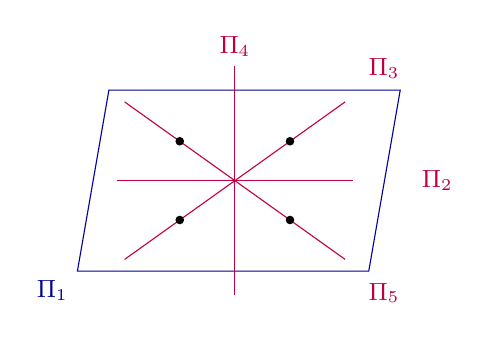
\begin{tikzpicture}
\draw[blue!60!black](-2,-1.15)--(1.7,-1.15)--(2.1,1.15)--(-1.6,1.15)--cycle;
\node[blue!60!black,below left]at(-2,-1.15){$\Pi_1$};
\draw[purple](-1.5,0)--(1.5,0);\node[purple,right]at(2.25,0){$\Pi_2$};
\draw[purple](0,-1.45)--(0,1.45)node[above]{$\Pi_4$};
\draw[purple](-1.4,-1)--(1.4,1)node[above right=5pt]{$\Pi_3$};
\draw[purple](-1.4,1)--(1.4,-1)node[below right=5pt]{$\Pi_5$};
\foreach\x/\y in{-.7/-.5,-.7/.5,.7/-.5,.7/.5}{\node[pt]at(\x,\y){};}
\end{tikzpicture}}
\Needspace{65mm}\titr{Une charge $+3q$ entourée de trois charges $-q$}
\fig{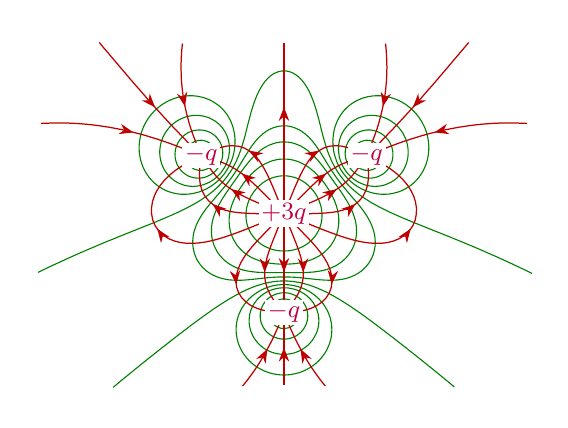
\begin{tikzpicture}[scale=1.05]
\clip (-3.1,-2.25) rectangle (3.1,2.25);
\draw[green!50!black,thin] plot coordinates {(-0.084,-1.368) (-0.108,-1.353) (-0.133,-1.332) (-0.156,-1.300) (-0.168,-1.278) (-0.179,-1.233) (-0.180,-1.189) (-0.169,-1.144) (-0.157,-1.120) (-0.133,-1.088) (-0.108,-1.066) (-0.084,-1.051) (-0.036,-1.034) (-0.012,-1.031) (0.028,-1.033) (0.060,-1.040) (0.092,-1.056) (0.123,-1.078) (0.143,-1.100) (0.158,-1.122) (0.176,-1.167) (0.181,-1.211) (0.175,-1.256) (0.157,-1.299) (0.141,-1.322) (0.119,-1.344) (0.087,-1.367) (0.060,-1.379) (0.012,-1.388) (-0.036,-1.386) (-0.084,-1.368)};
\draw[green!50!black,thin] plot coordinates {(-1.072,0.534) (-1.096,0.545) (-1.127,0.567) (-1.149,0.589) (-1.169,0.619) (-1.184,0.656) (-1.190,0.700) (-1.186,0.744) (-1.169,0.789) (-1.156,0.811) (-1.137,0.833) (-1.111,0.856) (-1.072,0.876) (-1.048,0.884) (-1.000,0.889) (-0.952,0.880) (-0.928,0.871) (-0.902,0.856) (-0.876,0.833) (-0.855,0.807) (-0.835,0.767) (-0.829,0.744) (-0.825,0.700) (-0.831,0.663) (-0.841,0.633) (-0.855,0.607) (-0.880,0.577) (-0.904,0.556) (-0.928,0.542) (-0.976,0.526) (-1.024,0.523) (-1.072,0.534)};
\draw[green!50!black,thin] plot coordinates {(0.928,0.542) (0.904,0.556) (0.880,0.577) (0.855,0.607) (0.841,0.633) (0.831,0.663) (0.825,0.700) (0.829,0.744) (0.835,0.767) (0.855,0.807) (0.876,0.833) (0.902,0.856) (0.928,0.871) (0.952,0.880) (1.000,0.889) (1.048,0.884) (1.072,0.876) (1.111,0.856) (1.137,0.833) (1.156,0.811) (1.169,0.789) (1.186,0.744) (1.190,0.700) (1.184,0.656) (1.169,0.619) (1.149,0.589) (1.127,0.567) (1.096,0.545) (1.072,0.534) (1.024,0.523) (0.976,0.526) (0.928,0.542)};
\draw[green!50!black,thin] plot coordinates {(-0.084,-1.505) (-0.108,-1.496) (-0.146,-1.478) (-0.179,-1.456) (-0.204,-1.433) (-0.225,-1.411) (-0.241,-1.389) (-0.254,-1.367) (-0.274,-1.322) (-0.280,-1.300) (-0.287,-1.256) (-0.287,-1.211) (-0.279,-1.167) (-0.273,-1.144) (-0.253,-1.102) (-0.238,-1.078) (-0.221,-1.056) (-0.199,-1.033) (-0.172,-1.011) (-0.135,-0.989) (-0.108,-0.976) (-0.077,-0.967) (-0.036,-0.958) (0.012,-0.956) (0.060,-0.962) (0.084,-0.968) (0.133,-0.987) (0.157,-1.001) (0.181,-1.018) (0.205,-1.039) (0.229,-1.066) (0.252,-1.100) (0.264,-1.122) (0.277,-1.160) (0.284,-1.189) (0.288,-1.233) (0.285,-1.278) (0.277,-1.310) (0.265,-1.344) (0.253,-1.369) (0.229,-1.406) (0.205,-1.433) (0.181,-1.454) (0.157,-1.472) (0.133,-1.485) (0.098,-1.500) (0.060,-1.511) (0.012,-1.517) (-0.036,-1.515) (-0.084,-1.505)};
\draw[green!50!black,thin] plot coordinates {(-1.072,0.432) (-1.096,0.436) (-1.145,0.451) (-1.169,0.463) (-1.193,0.478) (-1.222,0.500) (-1.245,0.522) (-1.265,0.548) (-1.289,0.589) (-1.299,0.611) (-1.312,0.656) (-1.316,0.678) (-1.318,0.722) (-1.314,0.767) (-1.309,0.789) (-1.294,0.833) (-1.283,0.856) (-1.265,0.885) (-1.241,0.916) (-1.217,0.939) (-1.193,0.959) (-1.169,0.974) (-1.138,0.989) (-1.096,1.004) (-1.055,1.011) (-1.024,1.013) (-0.990,1.011) (-0.952,1.005) (-0.907,0.989) (-0.880,0.975) (-0.855,0.959) (-0.831,0.940) (-0.807,0.915) (-0.783,0.881) (-0.769,0.856) (-0.759,0.833) (-0.746,0.789) (-0.740,0.744) (-0.742,0.700) (-0.750,0.656) (-0.759,0.628) (-0.776,0.589) (-0.789,0.567) (-0.807,0.542) (-0.831,0.515) (-0.855,0.494) (-0.880,0.477) (-0.919,0.456) (-0.952,0.442) (-0.994,0.433) (-1.024,0.430) (-1.072,0.432)};
\draw[green!50!black,thin] plot coordinates {(1.000,0.432) (0.976,0.436) (0.928,0.451) (0.904,0.462) (0.878,0.478) (0.848,0.500) (0.824,0.522) (0.805,0.544) (0.783,0.577) (0.765,0.611) (0.757,0.633) (0.745,0.678) (0.740,0.722) (0.742,0.767) (0.751,0.811) (0.759,0.833) (0.781,0.878) (0.796,0.900) (0.814,0.922) (0.837,0.944) (0.866,0.967) (0.904,0.987) (0.928,0.997) (0.976,1.009) (1.000,1.012) (1.048,1.012) (1.072,1.009) (1.120,0.996) (1.145,0.986) (1.180,0.967) (1.211,0.944) (1.235,0.922) (1.254,0.900) (1.270,0.878) (1.289,0.843) (1.303,0.811) (1.313,0.769) (1.317,0.744) (1.318,0.700) (1.313,0.663) (1.307,0.633) (1.289,0.589) (1.278,0.567) (1.263,0.544) (1.241,0.518) (1.217,0.495) (1.193,0.477) (1.154,0.456) (1.120,0.442) (1.080,0.433) (1.048,0.430) (1.000,0.432)};
\draw[green!50!black,thin] plot coordinates {(-0.012,-1.701) (-0.036,-1.700) (-0.084,-1.693) (-0.133,-1.681) (-0.157,-1.672) (-0.194,-1.656) (-0.229,-1.636) (-0.253,-1.620) (-0.277,-1.601) (-0.301,-1.579) (-0.325,-1.553) (-0.349,-1.522) (-0.364,-1.500) (-0.376,-1.478) (-0.396,-1.433) (-0.404,-1.411) (-0.415,-1.367) (-0.421,-1.322) (-0.422,-1.300) (-0.421,-1.278) (-0.417,-1.233) (-0.407,-1.189) (-0.398,-1.162) (-0.381,-1.122) (-0.369,-1.100) (-0.349,-1.071) (-0.325,-1.040) (-0.301,-1.015) (-0.277,-0.994) (-0.253,-0.975) (-0.229,-0.959) (-0.202,-0.944) (-0.157,-0.924) (-0.133,-0.916) (-0.084,-0.904) (-0.060,-0.900) (-0.012,-0.896) (0.036,-0.897) (0.061,-0.900) (0.108,-0.909) (0.151,-0.922) (0.181,-0.934) (0.205,-0.946) (0.241,-0.967) (0.272,-0.989) (0.297,-1.011) (0.319,-1.033) (0.338,-1.056) (0.355,-1.078) (0.373,-1.109) (0.391,-1.144) (0.400,-1.167) (0.413,-1.211) (0.420,-1.256) (0.422,-1.298) (0.422,-1.301) (0.419,-1.344) (0.411,-1.389) (0.398,-1.430) (0.387,-1.456) (0.373,-1.483) (0.349,-1.522) (0.333,-1.544) (0.313,-1.567) (0.291,-1.589) (0.265,-1.611) (0.233,-1.633) (0.205,-1.650) (0.181,-1.662) (0.141,-1.678) (0.108,-1.688) (0.060,-1.697) (0.034,-1.700) (-0.012,-1.701)};
\draw[green!50!black,thin] plot coordinates {(-1.193,0.341) (-1.217,0.348) (-1.265,0.366) (-1.289,0.378) (-1.313,0.392) (-1.341,0.411) (-1.368,0.433) (-1.390,0.456) (-1.410,0.478) (-1.434,0.511) (-1.454,0.544) (-1.465,0.567) (-1.482,0.611) (-1.488,0.633) (-1.498,0.678) (-1.502,0.722) (-1.502,0.767) (-1.497,0.811) (-1.488,0.856) (-1.482,0.878) (-1.465,0.922) (-1.454,0.944) (-1.434,0.981) (-1.413,1.011) (-1.395,1.033) (-1.375,1.056) (-1.352,1.078) (-1.324,1.100) (-1.292,1.122) (-1.265,1.138) (-1.241,1.150) (-1.198,1.167) (-1.169,1.176) (-1.120,1.185) (-1.079,1.189) (-1.048,1.189) (-1.024,1.188) (-0.976,1.181) (-0.928,1.167) (-0.904,1.159) (-0.874,1.144) (-0.836,1.122) (-0.807,1.101) (-0.783,1.080) (-0.760,1.056) (-0.741,1.033) (-0.726,1.011) (-0.711,0.987) (-0.690,0.944) (-0.682,0.922) (-0.669,0.878) (-0.663,0.839) (-0.660,0.811) (-0.659,0.767) (-0.663,0.730) (-0.667,0.700) (-0.678,0.656) (-0.687,0.630) (-0.704,0.589) (-0.715,0.567) (-0.735,0.534) (-0.759,0.501) (-0.778,0.478) (-0.800,0.456) (-0.824,0.433) (-0.853,0.411) (-0.880,0.394) (-0.904,0.380) (-0.932,0.367) (-0.976,0.350) (-1.000,0.343) (-1.048,0.334) (-1.096,0.330) (-1.145,0.333) (-1.193,0.341)};
\draw[green!50!black,thin] plot coordinates {(1.000,0.343) (0.976,0.350) (0.932,0.367) (0.904,0.380) (0.880,0.394) (0.853,0.411) (0.824,0.433) (0.800,0.456) (0.778,0.478) (0.759,0.501) (0.735,0.534) (0.715,0.567) (0.704,0.589) (0.687,0.630) (0.678,0.656) (0.667,0.700) (0.663,0.730) (0.659,0.767) (0.660,0.811) (0.663,0.839) (0.669,0.878) (0.682,0.922) (0.690,0.944) (0.711,0.987) (0.726,1.011) (0.741,1.033) (0.760,1.056) (0.783,1.080) (0.807,1.101) (0.836,1.122) (0.874,1.144) (0.904,1.159) (0.928,1.167) (0.976,1.181) (1.024,1.188) (1.048,1.189) (1.079,1.189) (1.120,1.185) (1.169,1.176) (1.198,1.167) (1.241,1.150) (1.265,1.138) (1.292,1.122) (1.324,1.100) (1.352,1.078) (1.375,1.056) (1.395,1.033) (1.413,1.011) (1.434,0.981) (1.454,0.944) (1.465,0.922) (1.482,0.878) (1.488,0.856) (1.497,0.811) (1.502,0.767) (1.502,0.722) (1.498,0.678) (1.488,0.633) (1.482,0.611) (1.465,0.567) (1.454,0.544) (1.434,0.511) (1.410,0.478) (1.390,0.456) (1.368,0.433) (1.341,0.411) (1.313,0.392) (1.289,0.378) (1.265,0.366) (1.217,0.348) (1.193,0.341) (1.145,0.333) (1.096,0.330) (1.048,0.334) (1.000,0.343)};
\draw[green!50!black,thin] plot coordinates {(-0.084,-1.945) (-0.108,-1.941) (-0.157,-1.930) (-0.184,-1.922) (-0.229,-1.906) (-0.253,-1.895) (-0.287,-1.878) (-0.325,-1.856) (-0.349,-1.839) (-0.373,-1.821) (-0.398,-1.800) (-0.422,-1.777) (-0.446,-1.751) (-0.469,-1.722) (-0.485,-1.700) (-0.500,-1.678) (-0.518,-1.646) (-0.535,-1.611) (-0.544,-1.589) (-0.559,-1.544) (-0.566,-1.515) (-0.573,-1.478) (-0.578,-1.433) (-0.579,-1.389) (-0.576,-1.344) (-0.569,-1.300) (-0.564,-1.278) (-0.551,-1.233) (-0.542,-1.211) (-0.522,-1.167) (-0.510,-1.144) (-0.494,-1.119) (-0.470,-1.085) (-0.446,-1.056) (-0.425,-1.033) (-0.402,-1.011) (-0.376,-0.989) (-0.349,-0.969) (-0.325,-0.953) (-0.301,-0.938) (-0.272,-0.922) (-0.229,-0.903) (-0.205,-0.893) (-0.157,-0.878) (-0.133,-0.872) (-0.084,-0.863) (-0.036,-0.858) (0.012,-0.857) (0.060,-0.860) (0.108,-0.867) (0.155,-0.878) (0.181,-0.885) (0.223,-0.900) (0.253,-0.913) (0.277,-0.925) (0.312,-0.944) (0.346,-0.967) (0.373,-0.987) (0.398,-1.008) (0.422,-1.030) (0.445,-1.056) (0.464,-1.078) (0.481,-1.100) (0.496,-1.122) (0.518,-1.160) (0.533,-1.189) (0.542,-1.212) (0.558,-1.256) (0.566,-1.290) (0.573,-1.322) (0.578,-1.367) (0.579,-1.411) (0.576,-1.456) (0.570,-1.500) (0.565,-1.522) (0.552,-1.567) (0.542,-1.593) (0.524,-1.633) (0.513,-1.656) (0.494,-1.687) (0.470,-1.721) (0.451,-1.744) (0.432,-1.767) (0.410,-1.789) (0.385,-1.811) (0.357,-1.833) (0.325,-1.855) (0.301,-1.870) (0.277,-1.883) (0.242,-1.900) (0.205,-1.915) (0.181,-1.923) (0.133,-1.936) (0.087,-1.944) (0.060,-1.948) (0.012,-1.951) (-0.036,-1.950) (-0.084,-1.945)};
\draw[green!50!black,thin] plot coordinates {(-1.337,0.250) (-1.361,0.256) (-1.410,0.273) (-1.434,0.283) (-1.467,0.300) (-1.504,0.322) (-1.530,0.341) (-1.554,0.360) (-1.578,0.382) (-1.602,0.406) (-1.626,0.433) (-1.643,0.456) (-1.658,0.478) (-1.675,0.505) (-1.696,0.544) (-1.706,0.567) (-1.722,0.611) (-1.729,0.633) (-1.740,0.678) (-1.747,0.721) (-1.750,0.744) (-1.752,0.789) (-1.751,0.833) (-1.747,0.874) (-1.743,0.900) (-1.734,0.944) (-1.723,0.985) (-1.714,1.011) (-1.699,1.049) (-1.685,1.078) (-1.674,1.100) (-1.651,1.138) (-1.631,1.167) (-1.615,1.189) (-1.596,1.211) (-1.576,1.233) (-1.554,1.256) (-1.529,1.278) (-1.501,1.300) (-1.470,1.322) (-1.435,1.344) (-1.410,1.358) (-1.386,1.370) (-1.340,1.389) (-1.313,1.399) (-1.267,1.411) (-1.241,1.417) (-1.193,1.424) (-1.145,1.427) (-1.096,1.426) (-1.048,1.421) (-1.000,1.411) (-0.976,1.405) (-0.928,1.389) (-0.904,1.379) (-0.879,1.367) (-0.841,1.344) (-0.808,1.322) (-0.783,1.303) (-0.759,1.281) (-0.735,1.257) (-0.715,1.233) (-0.698,1.211) (-0.682,1.189) (-0.663,1.156) (-0.645,1.122) (-0.636,1.100) (-0.620,1.056) (-0.613,1.033) (-0.603,0.989) (-0.596,0.944) (-0.592,0.900) (-0.592,0.856) (-0.595,0.811) (-0.600,0.767) (-0.609,0.722) (-0.615,0.700) (-0.629,0.656) (-0.639,0.631) (-0.657,0.589) (-0.668,0.567) (-0.687,0.534) (-0.709,0.500) (-0.725,0.478) (-0.743,0.456) (-0.763,0.433) (-0.785,0.411) (-0.809,0.389) (-0.835,0.367) (-0.865,0.344) (-0.900,0.322) (-0.928,0.306) (-0.952,0.294) (-0.989,0.278) (-1.024,0.264) (-1.055,0.256) (-1.096,0.245) (-1.145,0.238) (-1.193,0.235) (-1.241,0.235) (-1.289,0.240) (-1.337,0.250)};
\draw[green!50!black,thin] plot coordinates {(1.072,0.251) (1.048,0.257) (1.000,0.273) (0.976,0.283) (0.940,0.300) (0.904,0.320) (0.880,0.335) (0.855,0.351) (0.831,0.370) (0.807,0.390) (0.783,0.413) (0.759,0.438) (0.735,0.466) (0.711,0.498) (0.694,0.522) (0.681,0.544) (0.663,0.578) (0.646,0.611) (0.637,0.633) (0.622,0.678) (0.614,0.703) (0.604,0.744) (0.597,0.789) (0.593,0.833) (0.592,0.878) (0.594,0.922) (0.599,0.967) (0.607,1.011) (0.614,1.038) (0.627,1.078) (0.639,1.107) (0.656,1.144) (0.669,1.167) (0.687,1.196) (0.711,1.229) (0.734,1.256) (0.756,1.278) (0.780,1.300) (0.807,1.322) (0.831,1.339) (0.855,1.354) (0.880,1.367) (0.928,1.389) (0.952,1.398) (0.999,1.411) (1.024,1.417) (1.072,1.424) (1.120,1.427) (1.169,1.426) (1.217,1.421) (1.265,1.412) (1.289,1.406) (1.337,1.390) (1.361,1.381) (1.393,1.367) (1.434,1.345) (1.458,1.331) (1.482,1.314) (1.506,1.296) (1.530,1.277) (1.554,1.255) (1.578,1.231) (1.602,1.204) (1.627,1.173) (1.647,1.144) (1.661,1.122) (1.675,1.098) (1.696,1.056) (1.706,1.033) (1.722,0.989) (1.728,0.967) (1.739,0.922) (1.747,0.878) (1.749,0.856) (1.752,0.811) (1.751,0.767) (1.747,0.722) (1.744,0.700) (1.735,0.656) (1.723,0.614) (1.715,0.589) (1.699,0.552) (1.685,0.522) (1.672,0.500) (1.651,0.467) (1.627,0.434) (1.607,0.411) (1.586,0.389) (1.562,0.367) (1.535,0.344) (1.506,0.324) (1.482,0.309) (1.458,0.295) (1.421,0.278) (1.386,0.264) (1.358,0.256) (1.313,0.245) (1.265,0.237) (1.217,0.235) (1.169,0.236) (1.120,0.241) (1.072,0.251)};
\draw[green!50!black,thin] plot coordinates {(-2.066,-2.100) (-2.039,-2.078) (-2.013,-2.056) (-1.988,-2.035) (-1.964,-2.015) (-1.940,-1.995) (-1.916,-1.976) (-1.892,-1.956) (-1.867,-1.936) (-1.843,-1.917) (-1.819,-1.897) (-1.795,-1.877) (-1.768,-1.856) (-1.741,-1.833) (-1.713,-1.811) (-1.686,-1.789) (-1.658,-1.767) (-1.630,-1.744) (-1.602,-1.723) (-1.578,-1.704) (-1.554,-1.684) (-1.530,-1.665) (-1.506,-1.646) (-1.482,-1.627) (-1.458,-1.608) (-1.433,-1.589) (-1.405,-1.567) (-1.377,-1.544) (-1.348,-1.522) (-1.319,-1.500) (-1.291,-1.478) (-1.265,-1.458) (-1.241,-1.440) (-1.217,-1.421) (-1.193,-1.403) (-1.169,-1.385) (-1.145,-1.366) (-1.116,-1.344) (-1.086,-1.322) (-1.056,-1.300) (-1.026,-1.278) (-1.000,-1.259) (-0.976,-1.242) (-0.952,-1.224) (-0.928,-1.207) (-0.902,-1.189) (-0.871,-1.167) (-0.838,-1.144) (-0.807,-1.124) (-0.783,-1.108) (-0.759,-1.092) (-0.735,-1.077) (-0.702,-1.056) (-0.665,-1.033) (-0.639,-1.018) (-0.614,-1.004) (-0.588,-0.989) (-0.547,-0.967) (-0.518,-0.952) (-0.494,-0.940) (-0.456,-0.922) (-0.422,-0.907) (-0.398,-0.897) (-0.349,-0.878) (-0.325,-0.870) (-0.280,-0.856) (-0.253,-0.848) (-0.205,-0.836) (-0.181,-0.831) (-0.133,-0.823) (-0.084,-0.817) (-0.036,-0.814) (0.012,-0.813) (0.060,-0.815) (0.108,-0.820) (0.157,-0.827) (0.192,-0.833) (0.229,-0.842) (0.277,-0.855) (0.301,-0.862) (0.348,-0.878) (0.373,-0.888) (0.405,-0.900) (0.446,-0.918) (0.470,-0.929) (0.503,-0.944) (0.542,-0.964) (0.566,-0.977) (0.590,-0.990) (0.627,-1.011) (0.663,-1.032) (0.687,-1.047) (0.711,-1.062) (0.737,-1.078) (0.771,-1.100) (0.805,-1.122) (0.831,-1.140) (0.855,-1.157) (0.880,-1.173) (0.904,-1.190) (0.934,-1.211) (0.965,-1.233) (0.996,-1.256) (1.024,-1.277) (1.048,-1.294) (1.072,-1.312) (1.096,-1.330) (1.120,-1.348) (1.145,-1.367) (1.175,-1.389) (1.204,-1.411) (1.233,-1.433) (1.262,-1.456) (1.289,-1.477) (1.313,-1.495) (1.337,-1.514) (1.361,-1.533) (1.386,-1.552) (1.410,-1.571) (1.434,-1.589) (1.462,-1.611) (1.490,-1.633) (1.518,-1.656) (1.546,-1.678) (1.574,-1.700) (1.602,-1.722) (1.627,-1.742) (1.651,-1.761) (1.675,-1.780) (1.699,-1.800) (1.723,-1.819) (1.747,-1.839) (1.771,-1.858) (1.796,-1.878) (1.823,-1.900) (1.851,-1.922) (1.878,-1.944) (1.905,-1.967) (1.932,-1.989) (1.959,-2.011) (1.986,-2.033) (2.012,-2.055) (2.036,-2.075) (2.060,-2.095)};
\draw[green!50!black,thin] plot coordinates {(3.000,-0.722) (2.955,-0.700) (2.928,-0.687) (2.904,-0.675) (2.862,-0.656) (2.831,-0.641) (2.807,-0.630) (2.768,-0.611) (2.735,-0.596) (2.711,-0.585) (2.672,-0.567) (2.639,-0.552) (2.614,-0.541) (2.574,-0.522) (2.542,-0.508) (2.518,-0.498) (2.473,-0.478) (2.446,-0.466) (2.422,-0.455) (2.373,-0.434) (2.349,-0.424) (2.319,-0.411) (2.277,-0.393) (2.253,-0.383) (2.214,-0.367) (2.181,-0.353) (2.157,-0.343) (2.108,-0.323) (2.084,-0.313) (2.052,-0.300) (2.012,-0.284) (1.988,-0.274) (1.942,-0.256) (1.916,-0.245) (1.886,-0.233) (1.843,-0.216) (1.819,-0.207) (1.775,-0.189) (1.747,-0.178) (1.719,-0.167) (1.675,-0.149) (1.651,-0.139) (1.609,-0.122) (1.578,-0.110) (1.554,-0.100) (1.506,-0.080) (1.482,-0.070) (1.448,-0.056) (1.410,-0.040) (1.386,-0.029) (1.345,-0.011) (1.313,0.003) (1.289,0.014) (1.249,0.033) (1.217,0.049) (1.193,0.061) (1.160,0.078) (1.120,0.099) (1.096,0.112) (1.072,0.125) (1.041,0.144) (1.005,0.167) (0.976,0.185) (0.952,0.201) (0.928,0.218) (0.904,0.236) (0.879,0.256) (0.852,0.278) (0.827,0.300) (0.802,0.322) (0.780,0.344) (0.758,0.367) (0.735,0.392) (0.711,0.421) (0.687,0.452) (0.668,0.478) (0.653,0.500) (0.639,0.523) (0.614,0.564) (0.601,0.589) (0.589,0.611) (0.568,0.656) (0.559,0.678) (0.542,0.719) (0.532,0.744) (0.518,0.786) (0.509,0.811) (0.496,0.856) (0.489,0.878) (0.477,0.922) (0.470,0.950) (0.459,0.989) (0.448,1.033) (0.443,1.056) (0.431,1.100) (0.422,1.139) (0.414,1.167) (0.402,1.211) (0.396,1.233) (0.383,1.278) (0.373,1.308) (0.361,1.344) (0.349,1.377) (0.335,1.411) (0.325,1.435) (0.305,1.478) (0.294,1.500) (0.277,1.530) (0.253,1.567) (0.237,1.589) (0.219,1.611) (0.199,1.633) (0.175,1.656) (0.147,1.678) (0.111,1.700) (0.084,1.712) (0.050,1.722) (0.012,1.728) (-0.036,1.725) (-0.060,1.720) (-0.108,1.701) (-0.133,1.688) (-0.157,1.671) (-0.181,1.651) (-0.205,1.627) (-0.229,1.600) (-0.253,1.567) (-0.268,1.544) (-0.281,1.522) (-0.301,1.486) (-0.316,1.456) (-0.326,1.433) (-0.344,1.389) (-0.353,1.367) (-0.369,1.322) (-0.376,1.300) (-0.389,1.256) (-0.398,1.228) (-0.408,1.189) (-0.420,1.144) (-0.426,1.122) (-0.437,1.078) (-0.446,1.044) (-0.454,1.011) (-0.465,0.967) (-0.471,0.944) (-0.483,0.900) (-0.494,0.863) (-0.503,0.833) (-0.517,0.789) (-0.524,0.767) (-0.541,0.722) (-0.549,0.700) (-0.566,0.661) (-0.578,0.633) (-0.590,0.609) (-0.613,0.567) (-0.625,0.544) (-0.639,0.522) (-0.663,0.486) (-0.684,0.456) (-0.701,0.433) (-0.719,0.411) (-0.738,0.389) (-0.759,0.366) (-0.783,0.341) (-0.807,0.317) (-0.831,0.296) (-0.855,0.275) (-0.880,0.255) (-0.908,0.233) (-0.938,0.211) (-0.971,0.189) (-1.000,0.169) (-1.024,0.154) (-1.048,0.140) (-1.078,0.122) (-1.118,0.100) (-1.145,0.085) (-1.169,0.073) (-1.204,0.056) (-1.241,0.037) (-1.265,0.025) (-1.296,0.011) (-1.337,-0.008) (-1.361,-0.019) (-1.396,-0.033) (-1.434,-0.050) (-1.458,-0.060) (-1.500,-0.078) (-1.530,-0.090) (-1.554,-0.100) (-1.602,-0.120) (-1.627,-0.130) (-1.664,-0.144) (-1.699,-0.159) (-1.723,-0.168) (-1.771,-0.187) (-1.795,-0.197) (-1.831,-0.211) (-1.867,-0.226) (-1.892,-0.236) (-1.940,-0.255) (-1.964,-0.265) (-1.997,-0.278) (-2.036,-0.294) (-2.060,-0.304) (-2.106,-0.322) (-2.133,-0.333) (-2.160,-0.344) (-2.205,-0.363) (-2.229,-0.373) (-2.267,-0.389) (-2.301,-0.404) (-2.325,-0.414) (-2.371,-0.433) (-2.398,-0.445) (-2.423,-0.456) (-2.470,-0.476) (-2.494,-0.487) (-2.524,-0.500) (-2.566,-0.519) (-2.590,-0.530) (-2.623,-0.544) (-2.663,-0.563) (-2.687,-0.574) (-2.720,-0.589) (-2.759,-0.607) (-2.783,-0.618) (-2.815,-0.633) (-2.855,-0.652) (-2.880,-0.664) (-2.909,-0.678) (-2.952,-0.699) (-2.976,-0.710)};
\draw[green!50!black,thin] plot coordinates {(-0.711,-0.792) (-0.663,-0.800) (-0.614,-0.804) (-0.566,-0.805) (-0.518,-0.805) (-0.470,-0.802) (-0.422,-0.798) (-0.373,-0.793) (-0.333,-0.789) (-0.301,-0.785) (-0.253,-0.780) (-0.205,-0.775) (-0.157,-0.771) (-0.108,-0.768) (-0.084,-0.766) (-0.036,-0.765) (0.012,-0.765) (0.060,-0.765) (0.089,-0.767) (0.133,-0.769) (0.181,-0.773) (0.229,-0.777) (0.277,-0.783) (0.325,-0.788) (0.349,-0.791) (0.398,-0.796) (0.446,-0.800) (0.494,-0.803) (0.542,-0.805) (0.590,-0.805) (0.639,-0.802) (0.687,-0.796) (0.727,-0.789) (0.759,-0.781) (0.803,-0.767) (0.831,-0.755) (0.855,-0.744) (0.895,-0.722) (0.927,-0.700) (0.952,-0.680) (0.976,-0.658) (0.998,-0.633) (1.016,-0.611) (1.032,-0.589) (1.048,-0.562) (1.068,-0.522) (1.077,-0.500) (1.090,-0.456) (1.096,-0.427) (1.102,-0.389) (1.104,-0.344) (1.102,-0.300) (1.096,-0.261) (1.091,-0.233) (1.079,-0.189) (1.071,-0.167) (1.053,-0.122) (1.043,-0.100) (1.024,-0.065) (1.006,-0.033) (0.992,-0.011) (0.976,0.012) (0.952,0.046) (0.928,0.077) (0.910,0.100) (0.892,0.122) (0.873,0.144) (0.854,0.167) (0.831,0.193) (0.807,0.221) (0.783,0.249) (0.759,0.278) (0.741,0.300) (0.722,0.322) (0.704,0.344) (0.687,0.367) (0.663,0.398) (0.639,0.431) (0.621,0.456) (0.606,0.478) (0.590,0.501) (0.566,0.538) (0.548,0.567) (0.534,0.589) (0.518,0.615) (0.494,0.655) (0.480,0.678) (0.466,0.700) (0.446,0.733) (0.424,0.767) (0.409,0.789) (0.394,0.811) (0.373,0.840) (0.349,0.871) (0.325,0.899) (0.303,0.922) (0.280,0.944) (0.254,0.967) (0.229,0.986) (0.205,1.002) (0.181,1.016) (0.144,1.033) (0.108,1.047) (0.073,1.056) (0.036,1.062) (-0.012,1.063) (-0.060,1.058) (-0.084,1.053) (-0.133,1.038) (-0.157,1.028) (-0.190,1.011) (-0.225,0.989) (-0.253,0.968) (-0.277,0.947) (-0.301,0.924) (-0.324,0.900) (-0.343,0.878) (-0.361,0.856) (-0.378,0.833) (-0.398,0.806) (-0.422,0.771) (-0.438,0.744) (-0.452,0.722) (-0.470,0.694) (-0.493,0.656) (-0.507,0.633) (-0.520,0.611) (-0.542,0.576) (-0.562,0.544) (-0.576,0.522) (-0.591,0.500) (-0.614,0.465) (-0.637,0.433) (-0.653,0.411) (-0.670,0.389) (-0.687,0.367) (-0.711,0.336) (-0.735,0.307) (-0.759,0.278) (-0.778,0.256) (-0.797,0.233) (-0.816,0.211) (-0.835,0.189) (-0.855,0.165) (-0.880,0.136) (-0.904,0.107) (-0.927,0.078) (-0.945,0.056) (-0.961,0.033) (-0.977,0.011) (-1.000,-0.024) (-1.019,-0.056) (-1.032,-0.078) (-1.048,-0.112) (-1.063,-0.144) (-1.072,-0.170) (-1.086,-0.211) (-1.096,-0.256) (-1.099,-0.278) (-1.103,-0.322) (-1.103,-0.367) (-1.099,-0.411) (-1.095,-0.433) (-1.084,-0.478) (-1.072,-0.511) (-1.058,-0.544) (-1.046,-0.567) (-1.024,-0.600) (-1.000,-0.631) (-0.978,-0.656) (-0.954,-0.678) (-0.928,-0.699) (-0.904,-0.716) (-0.880,-0.731) (-0.855,-0.744) (-0.807,-0.765) (-0.783,-0.774) (-0.735,-0.787) (-0.711,-0.792)};
\draw[green!50!black,thin] plot coordinates {(-0.373,-0.703) (-0.325,-0.708) (-0.277,-0.710) (-0.229,-0.712) (-0.181,-0.713) (-0.133,-0.713) (-0.084,-0.713) (-0.036,-0.713) (0.012,-0.713) (0.060,-0.713) (0.108,-0.713) (0.157,-0.713) (0.205,-0.713) (0.253,-0.711) (0.301,-0.709) (0.349,-0.706) (0.397,-0.700) (0.422,-0.696) (0.470,-0.687) (0.505,-0.678) (0.542,-0.666) (0.570,-0.656) (0.614,-0.635) (0.639,-0.622) (0.663,-0.607) (0.689,-0.589) (0.716,-0.567) (0.740,-0.544) (0.761,-0.522) (0.783,-0.495) (0.807,-0.460) (0.823,-0.433) (0.834,-0.411) (0.852,-0.367) (0.859,-0.344) (0.869,-0.300) (0.876,-0.256) (0.878,-0.211) (0.876,-0.167) (0.871,-0.122) (0.862,-0.078) (0.855,-0.055) (0.841,-0.011) (0.831,0.015) (0.814,0.056) (0.803,0.078) (0.783,0.115) (0.767,0.144) (0.753,0.167) (0.735,0.196) (0.711,0.233) (0.696,0.256) (0.681,0.278) (0.663,0.304) (0.639,0.338) (0.618,0.367) (0.603,0.389) (0.587,0.411) (0.566,0.440) (0.542,0.474) (0.523,0.500) (0.507,0.522) (0.490,0.544) (0.470,0.571) (0.446,0.602) (0.422,0.631) (0.401,0.656) (0.380,0.678) (0.359,0.700) (0.336,0.722) (0.311,0.744) (0.283,0.767) (0.253,0.788) (0.229,0.803) (0.205,0.817) (0.169,0.833) (0.133,0.847) (0.102,0.856) (0.060,0.864) (0.012,0.868) (-0.036,0.867) (-0.084,0.860) (-0.108,0.854) (-0.157,0.838) (-0.181,0.828) (-0.215,0.811) (-0.252,0.789) (-0.277,0.771) (-0.301,0.753) (-0.325,0.732) (-0.349,0.710) (-0.373,0.685) (-0.398,0.659) (-0.420,0.633) (-0.438,0.611) (-0.456,0.589) (-0.473,0.567) (-0.494,0.539) (-0.518,0.507) (-0.539,0.478) (-0.555,0.456) (-0.571,0.433) (-0.590,0.406) (-0.614,0.372) (-0.634,0.344) (-0.650,0.322) (-0.665,0.300) (-0.687,0.269) (-0.711,0.233) (-0.725,0.211) (-0.740,0.189) (-0.759,0.157) (-0.779,0.122) (-0.792,0.100) (-0.807,0.069) (-0.824,0.033) (-0.833,0.011) (-0.849,-0.033) (-0.856,-0.056) (-0.867,-0.100) (-0.874,-0.144) (-0.877,-0.189) (-0.877,-0.233) (-0.873,-0.278) (-0.865,-0.322) (-0.855,-0.355) (-0.843,-0.389) (-0.831,-0.416) (-0.810,-0.456) (-0.796,-0.478) (-0.779,-0.500) (-0.759,-0.524) (-0.735,-0.549) (-0.711,-0.571) (-0.687,-0.590) (-0.656,-0.611) (-0.618,-0.633) (-0.590,-0.647) (-0.566,-0.657) (-0.518,-0.674) (-0.494,-0.681) (-0.446,-0.692) (-0.398,-0.700) (-0.373,-0.703)};
\draw[green!50!black,thin] plot coordinates {(-0.205,-0.593) (-0.157,-0.601) (-0.108,-0.606) (-0.060,-0.609) (-0.012,-0.611) (0.036,-0.610) (0.084,-0.608) (0.133,-0.604) (0.181,-0.597) (0.223,-0.589) (0.253,-0.582) (0.301,-0.568) (0.325,-0.559) (0.361,-0.544) (0.398,-0.526) (0.422,-0.513) (0.446,-0.497) (0.473,-0.478) (0.500,-0.456) (0.523,-0.433) (0.544,-0.411) (0.566,-0.383) (0.590,-0.348) (0.605,-0.322) (0.616,-0.300) (0.635,-0.256) (0.642,-0.233) (0.653,-0.189) (0.660,-0.144) (0.663,-0.114) (0.663,-0.078) (0.663,-0.056) (0.658,-0.011) (0.650,0.033) (0.639,0.078) (0.632,0.100) (0.616,0.144) (0.607,0.167) (0.590,0.202) (0.574,0.233) (0.562,0.256) (0.542,0.289) (0.521,0.322) (0.506,0.344) (0.490,0.367) (0.470,0.393) (0.446,0.422) (0.422,0.450) (0.398,0.475) (0.373,0.499) (0.349,0.520) (0.325,0.540) (0.301,0.559) (0.277,0.575) (0.253,0.590) (0.213,0.611) (0.181,0.626) (0.157,0.635) (0.108,0.649) (0.073,0.656) (0.036,0.660) (-0.012,0.661) (-0.060,0.658) (-0.084,0.654) (-0.133,0.643) (-0.161,0.633) (-0.205,0.615) (-0.229,0.604) (-0.255,0.589) (-0.290,0.567) (-0.320,0.544) (-0.347,0.522) (-0.372,0.500) (-0.395,0.478) (-0.416,0.456) (-0.436,0.433) (-0.455,0.411) (-0.473,0.389) (-0.494,0.361) (-0.518,0.326) (-0.535,0.300) (-0.549,0.278) (-0.566,0.248) (-0.586,0.211) (-0.597,0.189) (-0.614,0.148) (-0.625,0.122) (-0.639,0.079) (-0.645,0.056) (-0.655,0.011) (-0.661,-0.033) (-0.663,-0.059) (-0.663,-0.100) (-0.662,-0.122) (-0.657,-0.167) (-0.648,-0.211) (-0.639,-0.244) (-0.626,-0.278) (-0.614,-0.304) (-0.592,-0.344) (-0.578,-0.367) (-0.562,-0.389) (-0.542,-0.413) (-0.518,-0.438) (-0.494,-0.460) (-0.470,-0.480) (-0.442,-0.500) (-0.405,-0.522) (-0.373,-0.539) (-0.349,-0.549) (-0.304,-0.567) (-0.277,-0.575) (-0.229,-0.588) (-0.205,-0.593)};
\draw[green!50!black,thin] plot coordinates {(-0.133,-0.434) (-0.084,-0.445) (-0.036,-0.450) (0.012,-0.451) (0.060,-0.448) (0.108,-0.440) (0.135,-0.433) (0.181,-0.419) (0.205,-0.408) (0.243,-0.389) (0.277,-0.368) (0.301,-0.350) (0.325,-0.329) (0.349,-0.305) (0.372,-0.278) (0.388,-0.256) (0.402,-0.233) (0.422,-0.196) (0.434,-0.167) (0.446,-0.129) (0.453,-0.100) (0.459,-0.056) (0.460,-0.011) (0.457,0.033) (0.450,0.078) (0.444,0.100) (0.430,0.144) (0.421,0.167) (0.399,0.211) (0.386,0.233) (0.371,0.256) (0.349,0.284) (0.325,0.312) (0.301,0.336) (0.277,0.357) (0.253,0.376) (0.229,0.392) (0.194,0.411) (0.157,0.428) (0.133,0.437) (0.084,0.450) (0.046,0.456) (0.012,0.458) (-0.036,0.457) (-0.060,0.454) (-0.108,0.444) (-0.142,0.433) (-0.181,0.418) (-0.205,0.406) (-0.233,0.389) (-0.265,0.367) (-0.292,0.344) (-0.316,0.322) (-0.336,0.300) (-0.355,0.278) (-0.373,0.252) (-0.398,0.213) (-0.411,0.189) (-0.422,0.165) (-0.438,0.122) (-0.446,0.093) (-0.454,0.056) (-0.459,0.011) (-0.460,-0.033) (-0.456,-0.078) (-0.448,-0.122) (-0.442,-0.144) (-0.425,-0.189) (-0.415,-0.211) (-0.398,-0.241) (-0.373,-0.276) (-0.354,-0.300) (-0.333,-0.322) (-0.308,-0.344) (-0.279,-0.367) (-0.253,-0.383) (-0.229,-0.397) (-0.198,-0.411) (-0.157,-0.427) (-0.133,-0.434)};
\draw[field,line width=.45pt] plot coordinates {(0.120,0.000) (0.195,0.000) (0.270,0.000) (0.345,0.001) (0.420,0.004) (0.495,0.008) (0.570,0.015) (0.644,0.026) (0.716,0.044) (0.787,0.071) (0.852,0.107) (0.910,0.155) (0.957,0.213) (0.991,0.280) (1.012,0.352) (1.021,0.426) (1.022,0.501) (1.016,0.576)};
\draw[field,line width=.45pt] plot coordinates {(0.111,0.046) (0.180,0.075) (0.249,0.104) (0.318,0.133) (0.387,0.163) (0.455,0.195) (0.522,0.228) (0.588,0.264) (0.651,0.305) (0.711,0.349) (0.767,0.399) (0.819,0.453) (0.867,0.511) (0.912,0.571)};
\draw[field,line width=.45pt] plot coordinates {(0.085,0.085) (0.138,0.138) (0.191,0.191) (0.244,0.244) (0.297,0.297) (0.351,0.349) (0.406,0.400) (0.463,0.449) (0.522,0.495) (0.584,0.537) (0.649,0.575) (0.717,0.607) (0.787,0.634) (0.858,0.658)};
\draw[field,line width=.45pt] plot coordinates {(0.046,0.111) (0.075,0.180) (0.103,0.249) (0.132,0.319) (0.162,0.387) (0.193,0.456) (0.227,0.523) (0.264,0.588) (0.306,0.650) (0.355,0.707) (0.412,0.755) (0.477,0.793) (0.548,0.816) (0.623,0.823) (0.697,0.817) (0.770,0.800) (0.841,0.774) (0.910,0.744)};
\draw[field,line width=.45pt] plot coordinates {(0.000,0.120) (0.000,0.195) (0.000,0.270) (0.000,0.345) (0.000,0.420) (0.000,0.495) (0.000,0.570) (0.000,0.645) (0.000,0.720) (0.000,0.795) (0.000,0.870) (0.000,0.945) (0.000,1.020) (0.000,1.095) (0.000,1.170) (0.000,1.245) (0.000,1.320) (0.000,1.395) (0.000,1.470) (0.000,1.545) (0.000,1.620) (0.000,1.695) (0.000,1.770) (0.000,1.845) (0.000,1.920) (0.000,1.995) (0.000,2.070)};
\draw[field,line width=.45pt] plot coordinates {(-0.046,0.111) (-0.075,0.180) (-0.103,0.249) (-0.132,0.319) (-0.162,0.387) (-0.193,0.456) (-0.227,0.523) (-0.264,0.588) (-0.306,0.650) (-0.355,0.707) (-0.412,0.755) (-0.477,0.793) (-0.548,0.816) (-0.623,0.823) (-0.697,0.817) (-0.770,0.800) (-0.841,0.774) (-0.910,0.744)};
\draw[field,line width=.45pt] plot coordinates {(-0.085,0.085) (-0.138,0.138) (-0.191,0.191) (-0.244,0.244) (-0.297,0.297) (-0.351,0.349) (-0.406,0.400) (-0.463,0.449) (-0.522,0.495) (-0.584,0.537) (-0.649,0.575) (-0.717,0.607) (-0.787,0.634) (-0.858,0.658)};
\draw[field,line width=.45pt] plot coordinates {(-0.111,0.046) (-0.180,0.075) (-0.249,0.104) (-0.318,0.133) (-0.387,0.163) (-0.455,0.195) (-0.522,0.228) (-0.588,0.264) (-0.651,0.305) (-0.711,0.349) (-0.767,0.399) (-0.819,0.453) (-0.867,0.511) (-0.912,0.571)};
\draw[field,line width=.45pt] plot coordinates {(-0.120,0.000) (-0.195,0.000) (-0.270,0.000) (-0.345,0.001) (-0.420,0.004) (-0.495,0.008) (-0.570,0.015) (-0.644,0.026) (-0.716,0.044) (-0.787,0.071) (-0.852,0.107) (-0.910,0.155) (-0.957,0.213) (-0.991,0.280) (-1.012,0.352) (-1.021,0.426) (-1.022,0.501) (-1.016,0.576)};
\draw[field,line width=.45pt] plot coordinates {(-0.111,-0.046) (-0.180,-0.075) (-0.250,-0.103) (-0.319,-0.132) (-0.388,-0.160) (-0.458,-0.188) (-0.528,-0.215) (-0.598,-0.241) (-0.669,-0.266) (-0.740,-0.289) (-0.812,-0.311) (-0.885,-0.329) (-0.958,-0.344) (-1.033,-0.354) (-1.107,-0.359) (-1.182,-0.358) (-1.257,-0.348) (-1.329,-0.329) (-1.398,-0.300) (-1.461,-0.259) (-1.515,-0.207) (-1.558,-0.146) (-1.587,-0.077) (-1.601,-0.003) (-1.602,0.072) (-1.590,0.146) (-1.567,0.217) (-1.534,0.284) (-1.493,0.347) (-1.445,0.405) (-1.393,0.458) (-1.335,0.507) (-1.275,0.551) (-1.211,0.591) (-1.146,0.628)};
\draw[field,line width=.45pt] plot coordinates {(-0.085,-0.085) (-0.138,-0.138) (-0.191,-0.191) (-0.243,-0.245) (-0.295,-0.299) (-0.346,-0.354) (-0.395,-0.410) (-0.442,-0.469) (-0.485,-0.530) (-0.523,-0.595) (-0.553,-0.664) (-0.573,-0.736) (-0.581,-0.810) (-0.574,-0.885) (-0.549,-0.956) (-0.509,-1.019) (-0.456,-1.072) (-0.394,-1.114) (-0.326,-1.145) (-0.254,-1.167) (-0.181,-1.181) (-0.106,-1.191)};
\draw[field,line width=.45pt] plot coordinates {(-0.046,-0.111) (-0.075,-0.180) (-0.103,-0.250) (-0.131,-0.319) (-0.158,-0.389) (-0.183,-0.460) (-0.205,-0.531) (-0.222,-0.604) (-0.233,-0.679) (-0.234,-0.754) (-0.224,-0.828) (-0.203,-0.900) (-0.172,-0.968) (-0.133,-1.032) (-0.088,-1.092)};
\draw[field,line width=.45pt] plot coordinates {(-0.000,-0.120) (-0.000,-0.195) (-0.000,-0.270) (-0.000,-0.345) (-0.000,-0.420) (-0.000,-0.495) (-0.000,-0.570) (-0.000,-0.645) (-0.000,-0.720) (-0.000,-0.795) (-0.000,-0.870) (-0.000,-0.945) (-0.000,-1.020) (-0.000,-1.095)};
\draw[field,line width=.45pt] plot coordinates {(0.046,-0.111) (0.075,-0.180) (0.103,-0.250) (0.131,-0.319) (0.158,-0.389) (0.183,-0.460) (0.205,-0.531) (0.222,-0.604) (0.233,-0.679) (0.234,-0.754) (0.224,-0.828) (0.203,-0.900) (0.172,-0.968) (0.133,-1.032) (0.088,-1.092)};
\draw[field,line width=.45pt] plot coordinates {(0.085,-0.085) (0.138,-0.138) (0.191,-0.191) (0.243,-0.245) (0.295,-0.299) (0.346,-0.354) (0.395,-0.410) (0.442,-0.469) (0.485,-0.530) (0.523,-0.595) (0.553,-0.664) (0.573,-0.736) (0.581,-0.810) (0.574,-0.885) (0.549,-0.956) (0.509,-1.019) (0.456,-1.072) (0.394,-1.114) (0.326,-1.145) (0.254,-1.167) (0.181,-1.181) (0.106,-1.191)};
\draw[field,line width=.45pt] plot coordinates {(0.111,-0.046) (0.180,-0.075) (0.250,-0.103) (0.319,-0.132) (0.388,-0.160) (0.458,-0.188) (0.528,-0.215) (0.598,-0.241) (0.669,-0.266) (0.740,-0.289) (0.812,-0.311) (0.885,-0.329) (0.958,-0.344) (1.033,-0.354) (1.107,-0.359) (1.182,-0.358) (1.257,-0.348) (1.329,-0.329) (1.398,-0.300) (1.461,-0.259) (1.515,-0.207) (1.558,-0.146) (1.587,-0.077) (1.601,-0.003) (1.602,0.072) (1.590,0.146) (1.567,0.217) (1.534,0.284) (1.493,0.347) (1.445,0.405) (1.393,0.458) (1.335,0.507) (1.275,0.551) (1.211,0.591) (1.146,0.628)};
\draw[field,line width=.45pt] plot coordinates {(-1.228,2.058) (-1.236,1.984) (-1.241,1.909) (-1.244,1.834) (-1.245,1.759) (-1.243,1.684) (-1.240,1.609) (-1.233,1.534) (-1.225,1.460) (-1.214,1.386) (-1.200,1.312) (-1.184,1.239) (-1.166,1.166) (-1.146,1.094) (-1.124,1.022) (-1.099,0.951) (-1.073,0.881) (-1.046,0.811)};
\draw[field,line width=.45pt] plot coordinates {(-2.234,2.071) (-2.186,2.013) (-2.137,1.956) (-2.089,1.899) (-2.040,1.842) (-1.992,1.784) (-1.943,1.727) (-1.894,1.670) (-1.846,1.613) (-1.797,1.556) (-1.747,1.500) (-1.698,1.443) (-1.649,1.387) (-1.599,1.331) (-1.549,1.275) (-1.498,1.219) (-1.448,1.164) (-1.397,1.109) (-1.346,1.054) (-1.294,1.000) (-1.242,0.946) (-1.190,0.892) (-1.138,0.838) (-1.085,0.785)};
\draw[field,line width=.45pt] plot coordinates {(-2.937,1.092) (-2.862,1.095) (-2.787,1.097) (-2.712,1.098) (-2.637,1.097) (-2.562,1.094) (-2.487,1.090) (-2.412,1.084) (-2.338,1.077) (-2.263,1.068) (-2.189,1.057) (-2.115,1.046) (-2.041,1.032) (-1.967,1.018) (-1.894,1.002) (-1.821,0.984) (-1.749,0.966) (-1.676,0.946) (-1.604,0.924) (-1.533,0.902) (-1.462,0.878) (-1.391,0.854) (-1.320,0.828) (-1.250,0.801) (-1.180,0.774) (-1.111,0.746)};
\draw[field,line width=.45pt] plot coordinates {(2.937,1.092) (2.862,1.095) (2.787,1.097) (2.712,1.098) (2.637,1.097) (2.562,1.094) (2.487,1.090) (2.412,1.084) (2.338,1.077) (2.263,1.068) (2.189,1.057) (2.115,1.046) (2.041,1.032) (1.967,1.018) (1.894,1.002) (1.821,0.984) (1.749,0.966) (1.676,0.946) (1.604,0.924) (1.533,0.902) (1.462,0.878) (1.391,0.854) (1.320,0.828) (1.250,0.801) (1.180,0.774) (1.111,0.746)};
\draw[field,line width=.45pt] plot coordinates {(2.234,2.071) (2.186,2.013) (2.137,1.956) (2.089,1.899) (2.040,1.842) (1.992,1.784) (1.943,1.727) (1.894,1.670) (1.846,1.613) (1.797,1.556) (1.747,1.500) (1.698,1.443) (1.649,1.387) (1.599,1.331) (1.549,1.275) (1.498,1.219) (1.448,1.164) (1.397,1.109) (1.346,1.054) (1.294,1.000) (1.242,0.946) (1.190,0.892) (1.138,0.838) (1.085,0.785)};
\draw[field,line width=.45pt] plot coordinates {(1.228,2.058) (1.236,1.984) (1.241,1.909) (1.244,1.834) (1.245,1.759) (1.243,1.684) (1.240,1.609) (1.233,1.534) (1.225,1.460) (1.214,1.386) (1.200,1.312) (1.184,1.239) (1.166,1.166) (1.146,1.094) (1.124,1.022) (1.099,0.951) (1.073,0.881) (1.046,0.811)};
\draw[field,line width=.45pt] plot coordinates {(-0.500,-2.084) (-0.453,-2.026) (-0.408,-1.966) (-0.364,-1.905) (-0.322,-1.843) (-0.282,-1.779) (-0.244,-1.715) (-0.207,-1.649) (-0.172,-1.583) (-0.138,-1.516) (-0.106,-1.448) (-0.076,-1.380) (-0.046,-1.311)};
\draw[field,line width=.45pt] plot coordinates {(-0.000,-2.070) (-0.000,-1.995) (-0.000,-1.920) (-0.000,-1.845) (-0.000,-1.770) (-0.000,-1.695) (-0.000,-1.620) (-0.000,-1.545) (-0.000,-1.470) (-0.000,-1.395) (-0.000,-1.320)};
\draw[field,line width=.45pt] plot coordinates {(0.500,-2.084) (0.453,-2.026) (0.408,-1.966) (0.364,-1.905) (0.322,-1.843) (0.282,-1.779) (0.244,-1.715) (0.207,-1.649) (0.172,-1.583) (0.138,-1.516) (0.106,-1.448) (0.076,-1.380) (0.046,-1.311)};
\fill[white](0,0)circle(.13);
\node[fill=white,inner sep=1pt,text=purple]at(0,0){$+3q$};
\fill[white](-1,0.7)circle(.13);
\node[fill=white,inner sep=1pt,text=purple]at(-1,0.7){$-q$};
\fill[white](1,0.7)circle(.13);
\node[fill=white,inner sep=1pt,text=purple]at(1,0.7){$-q$};
\fill[white](0,-1.2)circle(.13);
\node[fill=white,inner sep=1pt,text=purple]at(0,-1.2){$-q$};
\end{tikzpicture}}
Il existe quatre plans de symétrie.
\fig{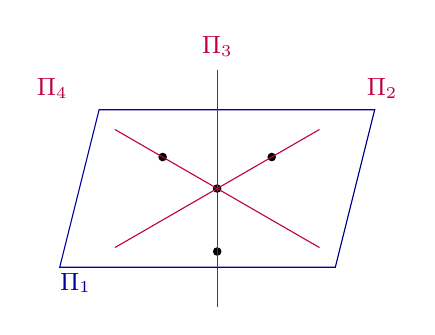
\begin{tikzpicture}\draw[blue!60!black](-2,-1)--(1.5,-1)--(2,1)--(-1.5,1)--cycle;\node[blue!60!black]at(-1.8,-1.2){$\Pi_1$};
\node[pt]at(0,0){};\foreach\a in{30,150,270}{\node[pt]at(\a:.8){};}
\draw[purple](30:1.5)--(210:1.5);\node[purple,above right]at(30:2.05){$\Pi_2$};
\draw[purple](90:1.5)--(270:1.5);\node[purple]at(90:1.8){$\Pi_3$};
\draw[purple](150:1.5)--(330:1.5);\node[purple,above left]at(150:2.05){$\Pi_4$};
\end{tikzpicture}}
La distribution est invariante par rotation d'angle $2\pi/3$ autour de $Oz$ : le champ présente une périodicité angulaire de $2\pi/3$.
\Needspace{65mm}\titr{Deux charges $+2q$ et $-q$}
\fig{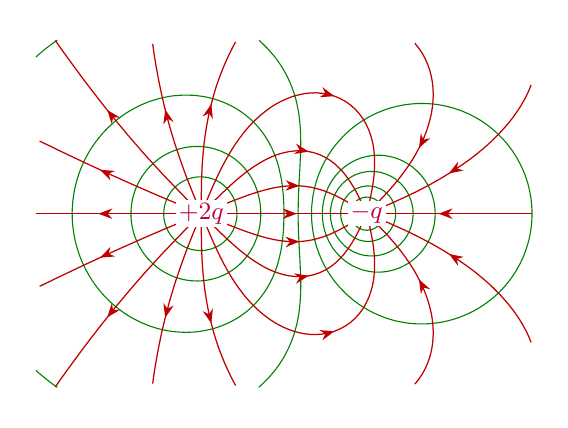
\begin{tikzpicture}[scale=1.05]
\clip (-3.1,-2.25) rectangle (3.1,2.25);
\draw[green!50!black,thin] plot coordinates {(0.952,-0.194) (0.928,-0.185) (0.893,-0.167) (0.865,-0.144) (0.845,-0.122) (0.831,-0.100) (0.812,-0.056) (0.807,-0.033) (0.804,0.011) (0.807,0.034) (0.819,0.078) (0.831,0.101) (0.855,0.134) (0.880,0.157) (0.904,0.174) (0.938,0.189) (0.976,0.199) (1.024,0.200) (1.070,0.189) (1.096,0.178) (1.120,0.163) (1.145,0.142) (1.169,0.113) (1.188,0.078) (1.196,0.056) (1.204,0.011) (1.202,-0.033) (1.193,-0.065) (1.178,-0.100) (1.163,-0.122) (1.142,-0.144) (1.115,-0.167) (1.072,-0.188) (1.048,-0.196) (1.000,-0.201) (0.952,-0.194)};
\draw[green!50!black,thin] plot coordinates {(0.928,-0.323) (0.904,-0.315) (0.870,-0.300) (0.832,-0.278) (0.807,-0.259) (0.783,-0.237) (0.760,-0.211) (0.743,-0.189) (0.730,-0.167) (0.711,-0.127) (0.701,-0.100) (0.690,-0.056) (0.687,-0.018) (0.686,0.011) (0.688,0.033) (0.695,0.078) (0.709,0.122) (0.718,0.144) (0.735,0.175) (0.759,0.210) (0.779,0.233) (0.803,0.256) (0.831,0.277) (0.855,0.293) (0.880,0.305) (0.926,0.322) (0.952,0.329) (1.000,0.335) (1.048,0.334) (1.096,0.326) (1.120,0.319) (1.166,0.300) (1.193,0.285) (1.217,0.269) (1.241,0.249) (1.265,0.225) (1.289,0.194) (1.307,0.167) (1.319,0.144) (1.336,0.100) (1.342,0.078) (1.350,0.033) (1.351,-0.011) (1.347,-0.056) (1.337,-0.094) (1.328,-0.122) (1.313,-0.154) (1.293,-0.189) (1.277,-0.211) (1.257,-0.233) (1.233,-0.256) (1.204,-0.278) (1.169,-0.299) (1.145,-0.310) (1.109,-0.322) (1.072,-0.331) (1.024,-0.336) (0.976,-0.333) (0.928,-0.323)};
\draw[green!50!black,thin] plot coordinates {(0.976,-0.504) (0.952,-0.500) (0.904,-0.486) (0.880,-0.477) (0.832,-0.456) (0.807,-0.442) (0.783,-0.426) (0.759,-0.409) (0.735,-0.389) (0.711,-0.366) (0.687,-0.340) (0.663,-0.310) (0.641,-0.278) (0.627,-0.256) (0.614,-0.230) (0.596,-0.189) (0.588,-0.167) (0.576,-0.122) (0.567,-0.078) (0.564,-0.056) (0.562,-0.011) (0.562,0.033) (0.566,0.070) (0.571,0.100) (0.581,0.144) (0.590,0.172) (0.605,0.211) (0.616,0.233) (0.639,0.274) (0.655,0.300) (0.672,0.322) (0.690,0.344) (0.711,0.367) (0.735,0.389) (0.762,0.411) (0.794,0.433) (0.831,0.455) (0.855,0.467) (0.881,0.478) (0.928,0.494) (0.954,0.500) (1.000,0.508) (1.048,0.511) (1.096,0.510) (1.145,0.504) (1.169,0.499) (1.217,0.485) (1.241,0.476) (1.287,0.456) (1.313,0.441) (1.337,0.426) (1.361,0.408) (1.386,0.388) (1.410,0.366) (1.434,0.340) (1.458,0.311) (1.481,0.278) (1.494,0.256) (1.506,0.233) (1.526,0.189) (1.534,0.167) (1.547,0.122) (1.554,0.086) (1.559,0.056) (1.562,0.011) (1.561,-0.033) (1.556,-0.078) (1.552,-0.100) (1.541,-0.144) (1.530,-0.177) (1.517,-0.211) (1.506,-0.233) (1.482,-0.276) (1.466,-0.300) (1.449,-0.322) (1.430,-0.344) (1.409,-0.367) (1.385,-0.389) (1.357,-0.411) (1.325,-0.433) (1.289,-0.454) (1.265,-0.466) (1.237,-0.478) (1.193,-0.493) (1.163,-0.500) (1.120,-0.508) (1.072,-0.511) (1.024,-0.510) (0.976,-0.504)};
\draw[green!50!black,thin] plot coordinates {(1.048,-0.701) (1.024,-0.697) (0.976,-0.687) (0.946,-0.678) (0.904,-0.663) (0.880,-0.653) (0.837,-0.633) (0.807,-0.617) (0.783,-0.602) (0.759,-0.586) (0.733,-0.567) (0.706,-0.544) (0.682,-0.522) (0.660,-0.500) (0.639,-0.477) (0.614,-0.447) (0.590,-0.414) (0.574,-0.389) (0.561,-0.367) (0.542,-0.332) (0.527,-0.300) (0.518,-0.278) (0.501,-0.233) (0.494,-0.210) (0.483,-0.167) (0.474,-0.122) (0.470,-0.093) (0.466,-0.056) (0.464,-0.011) (0.465,0.033) (0.468,0.078) (0.471,0.100) (0.478,0.144) (0.488,0.189) (0.494,0.211) (0.509,0.256) (0.518,0.279) (0.537,0.322) (0.548,0.344) (0.566,0.376) (0.588,0.411) (0.604,0.433) (0.621,0.456) (0.640,0.478) (0.663,0.503) (0.687,0.527) (0.711,0.548) (0.735,0.568) (0.764,0.589) (0.798,0.611) (0.831,0.630) (0.855,0.643) (0.885,0.656) (0.928,0.672) (0.952,0.680) (1.000,0.692) (1.044,0.700) (1.072,0.704) (1.120,0.707) (1.169,0.707) (1.217,0.703) (1.241,0.699) (1.289,0.690) (1.335,0.678) (1.361,0.669) (1.397,0.656) (1.434,0.639) (1.458,0.627) (1.485,0.611) (1.520,0.589) (1.551,0.567) (1.578,0.544) (1.602,0.523) (1.626,0.500) (1.647,0.478) (1.666,0.456) (1.684,0.433) (1.700,0.411) (1.723,0.375) (1.741,0.344) (1.753,0.322) (1.771,0.282) (1.782,0.256) (1.795,0.216) (1.803,0.189) (1.814,0.144) (1.819,0.114) (1.824,0.078) (1.828,0.033) (1.829,-0.011) (1.826,-0.056) (1.822,-0.100) (1.818,-0.122) (1.809,-0.167) (1.797,-0.211) (1.790,-0.233) (1.773,-0.278) (1.763,-0.300) (1.747,-0.333) (1.728,-0.367) (1.715,-0.389) (1.699,-0.412) (1.675,-0.445) (1.651,-0.473) (1.627,-0.499) (1.603,-0.522) (1.578,-0.544) (1.554,-0.564) (1.530,-0.582) (1.506,-0.598) (1.482,-0.613) (1.445,-0.633) (1.410,-0.650) (1.386,-0.660) (1.337,-0.677) (1.313,-0.684) (1.265,-0.695) (1.236,-0.700) (1.193,-0.705) (1.145,-0.707) (1.096,-0.706) (1.048,-0.701)};
\draw[green!50!black,thin] plot coordinates {(1.506,-1.324) (1.482,-1.321) (1.434,-1.313) (1.386,-1.303) (1.361,-1.298) (1.313,-1.286) (1.286,-1.278) (1.241,-1.264) (1.217,-1.255) (1.169,-1.237) (1.145,-1.227) (1.109,-1.211) (1.072,-1.194) (1.048,-1.181) (1.021,-1.167) (0.983,-1.144) (0.952,-1.126) (0.928,-1.110) (0.904,-1.094) (0.880,-1.076) (0.852,-1.056) (0.824,-1.033) (0.798,-1.011) (0.772,-0.989) (0.748,-0.967) (0.726,-0.944) (0.704,-0.922) (0.683,-0.900) (0.663,-0.877) (0.639,-0.849) (0.614,-0.819) (0.592,-0.789) (0.576,-0.767) (0.561,-0.744) (0.542,-0.717) (0.518,-0.678) (0.506,-0.656) (0.493,-0.633) (0.470,-0.589) (0.460,-0.567) (0.446,-0.536) (0.431,-0.500) (0.422,-0.477) (0.406,-0.433) (0.398,-0.409) (0.385,-0.367) (0.373,-0.325) (0.367,-0.300) (0.358,-0.256) (0.350,-0.211) (0.347,-0.189) (0.341,-0.144) (0.337,-0.100) (0.334,-0.056) (0.333,-0.011) (0.334,0.033) (0.335,0.078) (0.339,0.122) (0.344,0.167) (0.349,0.206) (0.354,0.233) (0.363,0.278) (0.373,0.322) (0.379,0.344) (0.391,0.389) (0.398,0.411) (0.414,0.456) (0.422,0.478) (0.440,0.522) (0.450,0.544) (0.470,0.588) (0.482,0.611) (0.494,0.635) (0.518,0.677) (0.532,0.700) (0.546,0.722) (0.566,0.753) (0.590,0.787) (0.608,0.811) (0.626,0.833) (0.644,0.856) (0.663,0.878) (0.687,0.904) (0.711,0.930) (0.735,0.954) (0.759,0.977) (0.783,0.999) (0.807,1.020) (0.831,1.039) (0.855,1.058) (0.882,1.078) (0.913,1.100) (0.947,1.122) (0.976,1.141) (1.000,1.155) (1.024,1.168) (1.063,1.189) (1.096,1.205) (1.120,1.216) (1.160,1.233) (1.193,1.246) (1.218,1.256) (1.265,1.272) (1.289,1.279) (1.337,1.292) (1.371,1.300) (1.410,1.308) (1.458,1.317) (1.495,1.322) (1.530,1.326) (1.578,1.330) (1.627,1.333) (1.675,1.333) (1.723,1.332) (1.771,1.329) (1.819,1.325) (1.843,1.322) (1.892,1.314) (1.940,1.305) (1.964,1.300) (2.012,1.288) (2.047,1.278) (2.084,1.266) (2.115,1.256) (2.157,1.240) (2.181,1.230) (2.224,1.211) (2.253,1.198) (2.277,1.185) (2.312,1.167) (2.349,1.145) (2.373,1.131) (2.398,1.115) (2.422,1.099) (2.452,1.078) (2.481,1.056) (2.509,1.033) (2.536,1.011) (2.561,0.989) (2.585,0.967) (2.608,0.944) (2.630,0.922) (2.651,0.900) (2.670,0.878) (2.689,0.856) (2.711,0.829) (2.735,0.798) (2.758,0.767) (2.773,0.744) (2.788,0.722) (2.807,0.691) (2.828,0.656) (2.840,0.633) (2.855,0.604) (2.874,0.567) (2.884,0.544) (2.903,0.500) (2.912,0.478) (2.928,0.433) (2.935,0.411) (2.949,0.367) (2.955,0.344) (2.966,0.300) (2.975,0.256) (2.979,0.233) (2.987,0.189) (2.992,0.144) (2.996,0.100) (2.999,0.056) (3.000,0.011) (3.000,-0.033) (2.998,-0.078) (2.994,-0.122) (2.990,-0.167) (2.983,-0.211) (2.976,-0.252) (2.971,-0.278) (2.961,-0.322) (2.952,-0.355) (2.942,-0.389) (2.928,-0.433) (2.920,-0.456) (2.904,-0.498) (2.894,-0.522) (2.880,-0.554) (2.863,-0.589) (2.852,-0.611) (2.831,-0.649) (2.815,-0.678) (2.802,-0.700) (2.783,-0.729) (2.759,-0.765) (2.742,-0.789) (2.725,-0.811) (2.708,-0.833) (2.687,-0.859) (2.663,-0.886) (2.639,-0.913) (2.614,-0.938) (2.590,-0.962) (2.566,-0.984) (2.542,-1.006) (2.518,-1.026) (2.494,-1.046) (2.470,-1.064) (2.446,-1.082) (2.420,-1.100) (2.387,-1.122) (2.351,-1.144) (2.325,-1.159) (2.301,-1.173) (2.270,-1.189) (2.229,-1.209) (2.205,-1.220) (2.173,-1.233) (2.133,-1.249) (2.108,-1.258) (2.060,-1.274) (2.036,-1.281) (1.988,-1.294) (1.963,-1.300) (1.916,-1.310) (1.867,-1.318) (1.838,-1.322) (1.795,-1.327) (1.747,-1.331) (1.699,-1.333) (1.651,-1.333) (1.602,-1.332) (1.554,-1.329) (1.506,-1.324)};
\draw[green!50!black,thin] plot coordinates {(-0.306,-2.100) (-0.281,-2.078) (-0.257,-2.056) (-0.234,-2.033) (-0.212,-2.011) (-0.191,-1.989) (-0.170,-1.967) (-0.151,-1.944) (-0.132,-1.922) (-0.108,-1.893) (-0.084,-1.861) (-0.064,-1.833) (-0.049,-1.811) (-0.035,-1.789) (-0.012,-1.753) (0.006,-1.722) (0.018,-1.700) (0.036,-1.665) (0.052,-1.633) (0.062,-1.611) (0.081,-1.567) (0.090,-1.544) (0.107,-1.500) (0.115,-1.478) (0.129,-1.433) (0.135,-1.411) (0.147,-1.367) (0.157,-1.328) (0.163,-1.300) (0.171,-1.256) (0.179,-1.211) (0.182,-1.189) (0.188,-1.144) (0.192,-1.100) (0.196,-1.056) (0.199,-1.011) (0.201,-0.967) (0.202,-0.922) (0.203,-0.878) (0.203,-0.833) (0.202,-0.789) (0.201,-0.744) (0.199,-0.700) (0.197,-0.656) (0.195,-0.611) (0.193,-0.567) (0.191,-0.522) (0.188,-0.478) (0.186,-0.433) (0.183,-0.389) (0.181,-0.344) (0.180,-0.322) (0.178,-0.278) (0.176,-0.233) (0.175,-0.189) (0.173,-0.144) (0.172,-0.100) (0.172,-0.056) (0.172,-0.011) (0.172,0.033) (0.172,0.078) (0.173,0.122) (0.174,0.167) (0.175,0.211) (0.177,0.256) (0.179,0.300) (0.181,0.337) (0.182,0.367) (0.185,0.411) (0.187,0.456) (0.189,0.500) (0.192,0.544) (0.194,0.589) (0.196,0.633) (0.198,0.678) (0.200,0.722) (0.201,0.767) (0.202,0.811) (0.203,0.856) (0.202,0.900) (0.202,0.944) (0.200,0.989) (0.198,1.033) (0.194,1.078) (0.190,1.122) (0.185,1.167) (0.181,1.198) (0.175,1.233) (0.167,1.278) (0.158,1.322) (0.153,1.344) (0.142,1.389) (0.133,1.421) (0.122,1.456) (0.108,1.496) (0.099,1.522) (0.084,1.559) (0.072,1.589) (0.060,1.615) (0.041,1.656) (0.030,1.678) (0.012,1.711) (-0.007,1.744) (-0.021,1.767) (-0.036,1.791) (-0.060,1.827) (-0.080,1.856) (-0.097,1.878) (-0.114,1.900) (-0.133,1.923) (-0.157,1.951) (-0.181,1.978) (-0.205,2.004) (-0.229,2.028) (-0.253,2.052) (-0.277,2.074) (-0.301,2.096)};
\draw[green!50!black,thin] plot coordinates {(-3.000,-1.895) (-2.976,-1.917) (-2.952,-1.938) (-2.928,-1.958) (-2.904,-1.978) (-2.880,-1.998) (-2.855,-2.017) (-2.831,-2.035) (-2.804,-2.056) (-2.773,-2.078) (-2.742,-2.100)};
\draw[green!50!black,thin] plot coordinates {(-2.742,2.100) (-2.773,2.078) (-2.804,2.056) (-2.831,2.035) (-2.855,2.017) (-2.880,1.998) (-2.904,1.978) (-2.928,1.958) (-2.952,1.938) (-2.976,1.917) (-3.000,1.895)};
\draw[green!50!black,thin] plot coordinates {(-1.241,-1.433) (-1.193,-1.435) (-1.145,-1.434) (-1.120,-1.433) (-1.072,-1.430) (-1.024,-1.424) (-0.976,-1.417) (-0.945,-1.411) (-0.904,-1.402) (-0.855,-1.390) (-0.831,-1.383) (-0.783,-1.367) (-0.759,-1.358) (-0.725,-1.344) (-0.687,-1.328) (-0.663,-1.317) (-0.630,-1.300) (-0.590,-1.278) (-0.566,-1.264) (-0.542,-1.249) (-0.518,-1.232) (-0.488,-1.211) (-0.459,-1.189) (-0.432,-1.167) (-0.407,-1.144) (-0.383,-1.122) (-0.360,-1.100) (-0.339,-1.078) (-0.319,-1.056) (-0.300,-1.033) (-0.277,-1.005) (-0.253,-0.973) (-0.233,-0.944) (-0.218,-0.922) (-0.205,-0.900) (-0.181,-0.859) (-0.167,-0.833) (-0.156,-0.811) (-0.135,-0.767) (-0.125,-0.744) (-0.108,-0.702) (-0.099,-0.678) (-0.084,-0.633) (-0.077,-0.611) (-0.065,-0.567) (-0.059,-0.544) (-0.049,-0.500) (-0.039,-0.456) (-0.035,-0.433) (-0.028,-0.389) (-0.021,-0.344) (-0.016,-0.300) (-0.012,-0.263) (-0.009,-0.233) (-0.006,-0.189) (-0.003,-0.144) (-0.002,-0.100) (-0.000,-0.056) (0.000,-0.011) (-0.000,0.033) (-0.001,0.078) (-0.002,0.122) (-0.005,0.167) (-0.008,0.211) (-0.011,0.256) (-0.014,0.278) (-0.018,0.322) (-0.024,0.367) (-0.031,0.411) (-0.036,0.438) (-0.044,0.478) (-0.054,0.522) (-0.060,0.549) (-0.071,0.589) (-0.084,0.633) (-0.092,0.656) (-0.107,0.700) (-0.116,0.722) (-0.133,0.761) (-0.145,0.789) (-0.157,0.813) (-0.179,0.856) (-0.191,0.878) (-0.205,0.900) (-0.229,0.938) (-0.248,0.967) (-0.265,0.989) (-0.282,1.011) (-0.301,1.035) (-0.325,1.063) (-0.349,1.089) (-0.373,1.113) (-0.398,1.136) (-0.422,1.158) (-0.446,1.178) (-0.470,1.197) (-0.494,1.215) (-0.519,1.233) (-0.553,1.256) (-0.590,1.278) (-0.614,1.292) (-0.639,1.305) (-0.674,1.322) (-0.711,1.339) (-0.735,1.349) (-0.782,1.367) (-0.807,1.375) (-0.852,1.389) (-0.880,1.396) (-0.928,1.408) (-0.952,1.413) (-1.000,1.421) (-1.048,1.427) (-1.096,1.432) (-1.128,1.433) (-1.169,1.435) (-1.217,1.434) (-1.244,1.433) (-1.289,1.430) (-1.337,1.426) (-1.386,1.419) (-1.429,1.411) (-1.458,1.405) (-1.506,1.394) (-1.530,1.387) (-1.578,1.373) (-1.602,1.365) (-1.651,1.348) (-1.675,1.338) (-1.713,1.322) (-1.747,1.307) (-1.771,1.295) (-1.805,1.278) (-1.843,1.256) (-1.867,1.242) (-1.892,1.227) (-1.917,1.211) (-1.950,1.189) (-1.980,1.167) (-2.009,1.144) (-2.036,1.123) (-2.060,1.103) (-2.084,1.081) (-2.108,1.059) (-2.133,1.036) (-2.157,1.011) (-2.178,0.989) (-2.198,0.967) (-2.217,0.944) (-2.236,0.922) (-2.253,0.900) (-2.277,0.869) (-2.301,0.835) (-2.317,0.811) (-2.332,0.789) (-2.349,0.761) (-2.372,0.722) (-2.384,0.700) (-2.398,0.675) (-2.418,0.633) (-2.429,0.611) (-2.446,0.572) (-2.457,0.544) (-2.470,0.511) (-2.482,0.478) (-2.494,0.441) (-2.503,0.411) (-2.515,0.367) (-2.521,0.344) (-2.531,0.300) (-2.539,0.256) (-2.543,0.233) (-2.549,0.189) (-2.555,0.144) (-2.558,0.100) (-2.561,0.056) (-2.562,0.011) (-2.561,-0.033) (-2.560,-0.078) (-2.557,-0.122) (-2.552,-0.167) (-2.546,-0.211) (-2.542,-0.238) (-2.535,-0.278) (-2.526,-0.322) (-2.518,-0.355) (-2.509,-0.389) (-2.496,-0.433) (-2.489,-0.456) (-2.474,-0.500) (-2.466,-0.522) (-2.448,-0.567) (-2.439,-0.589) (-2.422,-0.626) (-2.407,-0.656) (-2.396,-0.678) (-2.373,-0.719) (-2.359,-0.744) (-2.346,-0.767) (-2.325,-0.799) (-2.302,-0.833) (-2.287,-0.856) (-2.270,-0.878) (-2.253,-0.900) (-2.229,-0.930) (-2.205,-0.959) (-2.181,-0.986) (-2.157,-1.011) (-2.135,-1.033) (-2.112,-1.056) (-2.088,-1.078) (-2.063,-1.100) (-2.037,-1.122) (-2.012,-1.142) (-1.988,-1.161) (-1.964,-1.179) (-1.940,-1.196) (-1.916,-1.212) (-1.882,-1.233) (-1.845,-1.256) (-1.819,-1.270) (-1.795,-1.283) (-1.761,-1.300) (-1.723,-1.318) (-1.699,-1.328) (-1.659,-1.344) (-1.627,-1.357) (-1.598,-1.367) (-1.554,-1.381) (-1.525,-1.389) (-1.482,-1.400) (-1.434,-1.410) (-1.410,-1.415) (-1.361,-1.423) (-1.313,-1.428) (-1.265,-1.432) (-1.241,-1.433)};
\draw[green!50!black,thin] plot coordinates {(-1.096,-0.812) (-1.048,-0.814) (-1.000,-0.812) (-0.976,-0.810) (-0.928,-0.804) (-0.880,-0.794) (-0.855,-0.788) (-0.807,-0.774) (-0.783,-0.765) (-0.735,-0.745) (-0.711,-0.733) (-0.687,-0.721) (-0.651,-0.700) (-0.618,-0.678) (-0.590,-0.658) (-0.566,-0.639) (-0.542,-0.618) (-0.518,-0.595) (-0.494,-0.569) (-0.472,-0.544) (-0.454,-0.522) (-0.437,-0.500) (-0.422,-0.477) (-0.398,-0.439) (-0.382,-0.411) (-0.370,-0.389) (-0.350,-0.344) (-0.341,-0.322) (-0.325,-0.280) (-0.318,-0.256) (-0.306,-0.211) (-0.301,-0.189) (-0.292,-0.144) (-0.286,-0.100) (-0.282,-0.056) (-0.281,-0.011) (-0.281,0.033) (-0.284,0.078) (-0.289,0.122) (-0.296,0.167) (-0.301,0.191) (-0.311,0.233) (-0.325,0.278) (-0.332,0.300) (-0.349,0.344) (-0.359,0.367) (-0.373,0.395) (-0.394,0.433) (-0.407,0.456) (-0.422,0.478) (-0.446,0.511) (-0.470,0.542) (-0.491,0.567) (-0.512,0.589) (-0.535,0.611) (-0.560,0.633) (-0.588,0.656) (-0.614,0.676) (-0.639,0.692) (-0.663,0.707) (-0.690,0.722) (-0.734,0.744) (-0.759,0.756) (-0.788,0.767) (-0.831,0.781) (-0.859,0.789) (-0.904,0.799) (-0.952,0.807) (-0.990,0.811) (-1.024,0.813) (-1.072,0.813) (-1.114,0.811) (-1.145,0.808) (-1.193,0.801) (-1.241,0.790) (-1.265,0.784) (-1.313,0.768) (-1.337,0.759) (-1.373,0.744) (-1.410,0.727) (-1.434,0.714) (-1.458,0.700) (-1.493,0.678) (-1.524,0.656) (-1.552,0.633) (-1.578,0.611) (-1.602,0.589) (-1.624,0.567) (-1.645,0.544) (-1.664,0.522) (-1.681,0.500) (-1.699,0.476) (-1.723,0.441) (-1.741,0.411) (-1.753,0.389) (-1.771,0.353) (-1.785,0.322) (-1.795,0.297) (-1.810,0.256) (-1.819,0.225) (-1.829,0.189) (-1.838,0.144) (-1.843,0.110) (-1.847,0.078) (-1.850,0.033) (-1.851,-0.011) (-1.849,-0.056) (-1.845,-0.100) (-1.842,-0.122) (-1.834,-0.167) (-1.823,-0.211) (-1.817,-0.233) (-1.803,-0.278) (-1.794,-0.300) (-1.775,-0.344) (-1.765,-0.367) (-1.747,-0.400) (-1.727,-0.433) (-1.713,-0.456) (-1.698,-0.478) (-1.675,-0.508) (-1.651,-0.538) (-1.627,-0.564) (-1.602,-0.589) (-1.578,-0.611) (-1.554,-0.632) (-1.530,-0.651) (-1.506,-0.669) (-1.482,-0.685) (-1.458,-0.700) (-1.418,-0.722) (-1.386,-0.739) (-1.361,-0.750) (-1.318,-0.767) (-1.289,-0.777) (-1.246,-0.789) (-1.217,-0.796) (-1.169,-0.805) (-1.120,-0.811) (-1.096,-0.812)};
\draw[green!50!black,thin] plot coordinates {(-1.096,-0.437) (-1.048,-0.444) (-1.000,-0.446) (-0.952,-0.442) (-0.907,-0.433) (-0.880,-0.426) (-0.839,-0.411) (-0.807,-0.396) (-0.783,-0.383) (-0.759,-0.367) (-0.730,-0.344) (-0.705,-0.322) (-0.683,-0.300) (-0.663,-0.275) (-0.639,-0.241) (-0.621,-0.211) (-0.610,-0.189) (-0.592,-0.144) (-0.585,-0.122) (-0.575,-0.078) (-0.570,-0.033) (-0.569,0.011) (-0.572,0.056) (-0.580,0.100) (-0.590,0.138) (-0.600,0.167) (-0.614,0.198) (-0.634,0.233) (-0.648,0.256) (-0.665,0.278) (-0.687,0.304) (-0.711,0.328) (-0.735,0.349) (-0.759,0.367) (-0.794,0.389) (-0.831,0.408) (-0.855,0.418) (-0.904,0.433) (-0.928,0.438) (-0.976,0.445) (-1.024,0.446) (-1.072,0.442) (-1.114,0.433) (-1.145,0.425) (-1.181,0.411) (-1.217,0.394) (-1.241,0.381) (-1.265,0.365) (-1.292,0.344) (-1.317,0.322) (-1.338,0.300) (-1.361,0.272) (-1.386,0.237) (-1.401,0.211) (-1.412,0.189) (-1.430,0.144) (-1.437,0.122) (-1.447,0.078) (-1.453,0.033) (-1.454,-0.011) (-1.451,-0.056) (-1.443,-0.100) (-1.434,-0.132) (-1.422,-0.167) (-1.410,-0.194) (-1.388,-0.233) (-1.374,-0.256) (-1.357,-0.278) (-1.337,-0.301) (-1.313,-0.325) (-1.289,-0.347) (-1.262,-0.367) (-1.227,-0.389) (-1.193,-0.406) (-1.169,-0.416) (-1.120,-0.432) (-1.096,-0.437)};
\draw[field,line width=.45pt] plot coordinates {(-0.880,0.000) (-0.805,0.000) (-0.730,0.000) (-0.655,0.000) (-0.580,0.000) (-0.505,0.000) (-0.430,0.000) (-0.355,0.000) (-0.280,0.000) (-0.205,0.000) (-0.130,0.000) (-0.055,0.000) (0.020,0.000) (0.095,0.000) (0.170,0.000) (0.245,0.000) (0.320,0.000) (0.395,0.000) (0.470,0.000) (0.545,0.000) (0.620,0.000) (0.695,0.000) (0.770,0.000) (0.845,0.000)};
\draw[field,line width=.45pt] plot coordinates {(-0.889,0.046) (-0.820,0.074) (-0.750,0.103) (-0.681,0.131) (-0.611,0.158) (-0.541,0.185) (-0.471,0.211) (-0.400,0.236) (-0.328,0.259) (-0.257,0.280) (-0.184,0.299) (-0.111,0.315) (-0.037,0.327) (0.038,0.335) (0.113,0.339) (0.188,0.337) (0.262,0.330) (0.336,0.318) (0.409,0.300) (0.481,0.278) (0.551,0.251) (0.619,0.220) (0.686,0.187) (0.752,0.151) (0.817,0.113) (0.881,0.074)};
\draw[field,line width=.45pt] plot coordinates {(-0.915,0.085) (-0.862,0.138) (-0.808,0.190) (-0.755,0.242) (-0.700,0.294) (-0.645,0.345) (-0.589,0.395) (-0.532,0.443) (-0.473,0.490) (-0.413,0.535) (-0.351,0.578) (-0.288,0.617) (-0.222,0.654) (-0.154,0.686) (-0.085,0.713) (-0.013,0.735) (0.060,0.751) (0.135,0.760) (0.210,0.761) (0.284,0.754) (0.358,0.739) (0.429,0.715) (0.497,0.683) (0.560,0.644) (0.620,0.598) (0.674,0.546) (0.725,0.491) (0.770,0.431) (0.812,0.369) (0.851,0.305) (0.887,0.239) (0.920,0.172) (0.952,0.104)};
\draw[field,line width=.45pt] plot coordinates {(-0.954,0.111) (-0.925,0.180) (-0.896,0.249) (-0.866,0.318) (-0.835,0.386) (-0.804,0.454) (-0.771,0.522) (-0.737,0.589) (-0.701,0.655) (-0.664,0.720) (-0.625,0.784) (-0.584,0.847) (-0.541,0.908) (-0.496,0.968) (-0.448,1.026) (-0.398,1.082) (-0.345,1.135) (-0.290,1.186) (-0.232,1.233) (-0.172,1.278) (-0.109,1.319) (-0.043,1.355) (0.024,1.387) (0.094,1.414) (0.166,1.435) (0.240,1.451) (0.314,1.460) (0.389,1.462) (0.464,1.456) (0.538,1.443) (0.610,1.422) (0.679,1.393) (0.745,1.357) (0.806,1.314) (0.862,1.264) (0.912,1.208) (0.956,1.148) (0.993,1.083) (1.025,1.015) (1.050,0.944) (1.070,0.872) (1.084,0.798) (1.092,0.723) (1.096,0.649) (1.096,0.574) (1.092,0.499) (1.085,0.424) (1.075,0.350) (1.062,0.276) (1.047,0.202) (1.031,0.129)};
\draw[field,line width=.45pt] plot coordinates {(-1.000,0.120) (-1.000,0.195) (-0.999,0.270) (-0.998,0.345) (-0.996,0.420) (-0.993,0.495) (-0.990,0.570) (-0.985,0.645) (-0.979,0.719) (-0.972,0.794) (-0.964,0.869) (-0.954,0.943) (-0.943,1.017) (-0.930,1.091) (-0.916,1.165) (-0.901,1.238) (-0.883,1.311) (-0.864,1.384) (-0.844,1.456) (-0.822,1.528) (-0.798,1.599) (-0.773,1.669) (-0.745,1.739) (-0.717,1.808) (-0.686,1.877) (-0.654,1.945) (-0.621,2.012) (-0.585,2.078)};
\draw[field,line width=.45pt] plot coordinates {(-1.046,0.111) (-1.074,0.180) (-1.103,0.250) (-1.130,0.319) (-1.158,0.389) (-1.185,0.459) (-1.211,0.530) (-1.236,0.600) (-1.261,0.671) (-1.285,0.742) (-1.309,0.813) (-1.332,0.885) (-1.353,0.956) (-1.375,1.028) (-1.395,1.100) (-1.414,1.173) (-1.433,1.245) (-1.451,1.318) (-1.468,1.391) (-1.485,1.464) (-1.500,1.538) (-1.515,1.611) (-1.529,1.685) (-1.542,1.759) (-1.555,1.833) (-1.567,1.907) (-1.578,1.981) (-1.588,2.055)};
\draw[field,line width=.45pt] plot coordinates {(-1.085,0.085) (-1.138,0.138) (-1.191,0.191) (-1.243,0.245) (-1.295,0.299) (-1.347,0.353) (-1.399,0.407) (-1.451,0.461) (-1.502,0.516) (-1.553,0.571) (-1.603,0.627) (-1.654,0.682) (-1.704,0.738) (-1.753,0.795) (-1.802,0.851) (-1.851,0.908) (-1.900,0.965) (-1.948,1.023) (-1.996,1.080) (-2.044,1.138) (-2.091,1.196) (-2.138,1.255) (-2.185,1.313) (-2.231,1.372) (-2.277,1.432) (-2.323,1.491) (-2.369,1.551) (-2.414,1.610) (-2.459,1.670) (-2.503,1.731) (-2.548,1.791) (-2.592,1.852) (-2.636,1.912) (-2.680,1.973) (-2.723,2.034) (-2.766,2.096)};
\draw[field,line width=.45pt] plot coordinates {(-1.111,0.046) (-1.180,0.075) (-1.249,0.104) (-1.318,0.133) (-1.388,0.162) (-1.457,0.191) (-1.526,0.221) (-1.594,0.250) (-1.663,0.280) (-1.732,0.310) (-1.801,0.340) (-1.869,0.371) (-1.938,0.401) (-2.006,0.432) (-2.075,0.463) (-2.143,0.494) (-2.211,0.525) (-2.279,0.557) (-2.347,0.588) (-2.415,0.620) (-2.483,0.652) (-2.551,0.684) (-2.618,0.716) (-2.686,0.748) (-2.754,0.781) (-2.821,0.814) (-2.889,0.846) (-2.956,0.879)};
\draw[field,line width=.45pt] plot coordinates {(-1.120,0.000) (-1.195,0.000) (-1.270,0.000) (-1.345,0.000) (-1.420,0.000) (-1.495,0.000) (-1.570,0.000) (-1.645,0.000) (-1.720,0.000) (-1.795,0.000) (-1.870,0.000) (-1.945,0.000) (-2.020,0.000) (-2.095,0.000) (-2.170,0.000) (-2.245,0.000) (-2.320,0.000) (-2.395,0.000) (-2.470,0.000) (-2.545,0.000) (-2.620,0.000) (-2.695,0.000) (-2.770,0.000) (-2.845,0.000) (-2.920,0.000) (-2.995,0.000)};
\draw[field,line width=.45pt] plot coordinates {(-1.111,-0.046) (-1.180,-0.075) (-1.249,-0.104) (-1.318,-0.133) (-1.388,-0.162) (-1.457,-0.191) (-1.526,-0.221) (-1.594,-0.250) (-1.663,-0.280) (-1.732,-0.310) (-1.801,-0.340) (-1.869,-0.371) (-1.938,-0.401) (-2.006,-0.432) (-2.075,-0.463) (-2.143,-0.494) (-2.211,-0.525) (-2.279,-0.557) (-2.347,-0.588) (-2.415,-0.620) (-2.483,-0.652) (-2.551,-0.684) (-2.618,-0.716) (-2.686,-0.748) (-2.754,-0.781) (-2.821,-0.814) (-2.889,-0.846) (-2.956,-0.879)};
\draw[field,line width=.45pt] plot coordinates {(-1.085,-0.085) (-1.138,-0.138) (-1.191,-0.191) (-1.243,-0.245) (-1.295,-0.299) (-1.347,-0.353) (-1.399,-0.407) (-1.451,-0.461) (-1.502,-0.516) (-1.553,-0.571) (-1.603,-0.627) (-1.654,-0.682) (-1.704,-0.738) (-1.753,-0.795) (-1.802,-0.851) (-1.851,-0.908) (-1.900,-0.965) (-1.948,-1.023) (-1.996,-1.080) (-2.044,-1.138) (-2.091,-1.196) (-2.138,-1.255) (-2.185,-1.313) (-2.231,-1.372) (-2.277,-1.432) (-2.323,-1.491) (-2.369,-1.551) (-2.414,-1.610) (-2.459,-1.670) (-2.503,-1.731) (-2.548,-1.791) (-2.592,-1.852) (-2.636,-1.912) (-2.680,-1.973) (-2.723,-2.034) (-2.766,-2.096)};
\draw[field,line width=.45pt] plot coordinates {(-1.046,-0.111) (-1.074,-0.180) (-1.103,-0.250) (-1.130,-0.319) (-1.158,-0.389) (-1.185,-0.459) (-1.211,-0.530) (-1.236,-0.600) (-1.261,-0.671) (-1.285,-0.742) (-1.309,-0.813) (-1.332,-0.885) (-1.353,-0.956) (-1.375,-1.028) (-1.395,-1.100) (-1.414,-1.173) (-1.433,-1.245) (-1.451,-1.318) (-1.468,-1.391) (-1.485,-1.464) (-1.500,-1.538) (-1.515,-1.611) (-1.529,-1.685) (-1.542,-1.759) (-1.555,-1.833) (-1.567,-1.907) (-1.578,-1.981) (-1.588,-2.055)};
\draw[field,line width=.45pt] plot coordinates {(-1.000,-0.120) (-1.000,-0.195) (-0.999,-0.270) (-0.998,-0.345) (-0.996,-0.420) (-0.993,-0.495) (-0.990,-0.570) (-0.985,-0.645) (-0.979,-0.719) (-0.972,-0.794) (-0.964,-0.869) (-0.954,-0.943) (-0.943,-1.017) (-0.930,-1.091) (-0.916,-1.165) (-0.901,-1.238) (-0.883,-1.311) (-0.864,-1.384) (-0.844,-1.456) (-0.822,-1.528) (-0.798,-1.599) (-0.773,-1.669) (-0.745,-1.739) (-0.717,-1.808) (-0.686,-1.877) (-0.654,-1.945) (-0.621,-2.012) (-0.585,-2.078)};
\draw[field,line width=.45pt] plot coordinates {(-0.954,-0.111) (-0.925,-0.180) (-0.896,-0.249) (-0.866,-0.318) (-0.835,-0.386) (-0.804,-0.454) (-0.771,-0.522) (-0.737,-0.589) (-0.701,-0.655) (-0.664,-0.720) (-0.625,-0.784) (-0.584,-0.847) (-0.541,-0.908) (-0.496,-0.968) (-0.448,-1.026) (-0.398,-1.082) (-0.345,-1.135) (-0.290,-1.186) (-0.232,-1.233) (-0.172,-1.278) (-0.109,-1.319) (-0.043,-1.355) (0.024,-1.387) (0.094,-1.414) (0.166,-1.435) (0.240,-1.451) (0.314,-1.460) (0.389,-1.462) (0.464,-1.456) (0.538,-1.443) (0.610,-1.422) (0.679,-1.393) (0.745,-1.357) (0.806,-1.314) (0.862,-1.264) (0.912,-1.208) (0.956,-1.148) (0.993,-1.083) (1.025,-1.015) (1.050,-0.944) (1.070,-0.872) (1.084,-0.798) (1.092,-0.723) (1.096,-0.649) (1.096,-0.574) (1.092,-0.499) (1.085,-0.424) (1.075,-0.350) (1.062,-0.276) (1.047,-0.202) (1.031,-0.129)};
\draw[field,line width=.45pt] plot coordinates {(-0.915,-0.085) (-0.862,-0.138) (-0.808,-0.190) (-0.755,-0.242) (-0.700,-0.294) (-0.645,-0.345) (-0.589,-0.395) (-0.532,-0.443) (-0.473,-0.490) (-0.413,-0.535) (-0.351,-0.578) (-0.288,-0.617) (-0.222,-0.654) (-0.154,-0.686) (-0.085,-0.713) (-0.013,-0.735) (0.060,-0.751) (0.135,-0.760) (0.210,-0.761) (0.284,-0.754) (0.358,-0.739) (0.429,-0.715) (0.497,-0.683) (0.560,-0.644) (0.620,-0.598) (0.674,-0.546) (0.725,-0.491) (0.770,-0.431) (0.812,-0.369) (0.851,-0.305) (0.887,-0.239) (0.920,-0.172) (0.952,-0.104)};
\draw[field,line width=.45pt] plot coordinates {(-0.889,-0.046) (-0.820,-0.074) (-0.750,-0.103) (-0.681,-0.131) (-0.611,-0.158) (-0.541,-0.185) (-0.471,-0.211) (-0.400,-0.236) (-0.328,-0.259) (-0.257,-0.280) (-0.184,-0.299) (-0.111,-0.315) (-0.037,-0.327) (0.038,-0.335) (0.113,-0.339) (0.188,-0.337) (0.262,-0.330) (0.336,-0.318) (0.409,-0.300) (0.481,-0.278) (0.551,-0.251) (0.619,-0.220) (0.686,-0.187) (0.752,-0.151) (0.817,-0.113) (0.881,-0.074)};
\draw[field,line width=.45pt] plot coordinates {(2.995,0.000) (2.920,0.000) (2.845,0.000) (2.770,0.000) (2.695,0.000) (2.620,0.000) (2.545,0.000) (2.470,0.000) (2.395,0.000) (2.320,0.000) (2.245,0.000) (2.170,0.000) (2.095,0.000) (2.020,0.000) (1.945,0.000) (1.870,0.000) (1.795,0.000) (1.720,0.000) (1.645,0.000) (1.570,0.000) (1.495,0.000) (1.420,0.000) (1.345,0.000) (1.270,0.000) (1.195,0.000) (1.120,0.000)};
\draw[field,line width=.45pt] plot coordinates {(2.989,1.556) (2.961,1.487) (2.929,1.419) (2.893,1.353) (2.855,1.289) (2.813,1.226) (2.770,1.165) (2.724,1.106) (2.675,1.049) (2.625,0.993) (2.573,0.939) (2.520,0.886) (2.465,0.835) (2.408,0.786) (2.351,0.738) (2.292,0.691) (2.232,0.646) (2.171,0.603) (2.109,0.560) (2.047,0.519) (1.983,0.479) (1.919,0.440) (1.854,0.402) (1.789,0.365) (1.723,0.330) (1.657,0.295) (1.590,0.261) (1.522,0.228) (1.454,0.196) (1.386,0.165) (1.318,0.134) (1.249,0.104) (1.180,0.075) (1.111,0.046)};
\draw[field,line width=.45pt] plot coordinates {(1.583,2.061) (1.630,2.003) (1.672,1.941) (1.708,1.875) (1.738,1.807) (1.763,1.736) (1.782,1.663) (1.795,1.589) (1.803,1.515) (1.805,1.440) (1.803,1.365) (1.795,1.290) (1.784,1.216) (1.767,1.143) (1.747,1.071) (1.724,1.000) (1.697,0.930) (1.666,0.861) (1.633,0.794) (1.598,0.728) (1.560,0.663) (1.519,0.600) (1.477,0.538) (1.433,0.478) (1.387,0.418) (1.339,0.360) (1.290,0.303) (1.240,0.247) (1.189,0.193) (1.137,0.138) (1.085,0.085)};
\draw[field,line width=.45pt] plot coordinates {(1.583,-2.061) (1.630,-2.003) (1.672,-1.941) (1.708,-1.875) (1.738,-1.807) (1.763,-1.736) (1.782,-1.663) (1.795,-1.589) (1.803,-1.515) (1.805,-1.440) (1.803,-1.365) (1.795,-1.290) (1.784,-1.216) (1.767,-1.143) (1.747,-1.071) (1.724,-1.000) (1.697,-0.930) (1.666,-0.861) (1.633,-0.794) (1.598,-0.728) (1.560,-0.663) (1.519,-0.600) (1.477,-0.538) (1.433,-0.478) (1.387,-0.418) (1.339,-0.360) (1.290,-0.303) (1.240,-0.247) (1.189,-0.193) (1.137,-0.138) (1.085,-0.085)};
\draw[field,line width=.45pt] plot coordinates {(2.989,-1.556) (2.961,-1.487) (2.929,-1.419) (2.893,-1.353) (2.855,-1.289) (2.813,-1.226) (2.770,-1.165) (2.724,-1.106) (2.675,-1.049) (2.625,-0.993) (2.573,-0.939) (2.520,-0.886) (2.465,-0.835) (2.408,-0.786) (2.351,-0.738) (2.292,-0.691) (2.232,-0.646) (2.171,-0.603) (2.109,-0.560) (2.047,-0.519) (1.983,-0.479) (1.919,-0.440) (1.854,-0.402) (1.789,-0.365) (1.723,-0.330) (1.657,-0.295) (1.590,-0.261) (1.522,-0.228) (1.454,-0.196) (1.386,-0.165) (1.318,-0.134) (1.249,-0.104) (1.180,-0.075) (1.111,-0.046)};
\fill[white](-1,0)circle(.13);
\node[fill=white,inner sep=1pt,text=purple]at(-1,0){$+2q$};
\fill[white](1,0)circle(.13);
\node[fill=white,inner sep=1pt,text=purple]at(1,0){$-q$};
\end{tikzpicture}}
% Sources 29--37
\section{Énergie potentielle d'interaction électrostatique}
\subsection{Charge dans un champ extérieur}
\fig{\begin{tikzpicture}\draw[cur](0,1)--(1,1)node[above]{$\E_{\mathrm{ext}}$};\node[pt,label=below:$q$]at(2,0){};\end{tikzpicture}}
\[\vec F_{\mathrm{ext}\to q}=q\E_{\mathrm{ext}}=-q\grad V_{\mathrm{ext}}=-\grad(qV_{\mathrm{ext}}).\]
La force est conservative.
\begin{result}[3]\[E_p=qV_{\mathrm{ext}}+\cste.\]\end{result}
\begin{exemple}\examtitle{Exercice classique de première année}
\fig{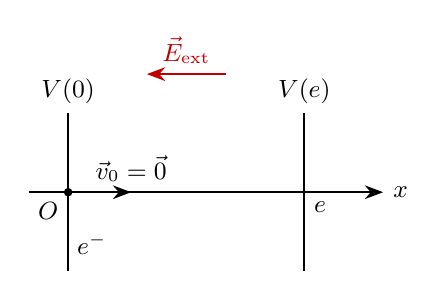
\begin{tikzpicture}\draw[thick](0,-1)--(0,1)(3,-1)--(3,1);\draw[arr](-.5,0)--(4,0)node[right]{$x$};\node[below left]at(0,0){$O$};\node[below right]at(3,0){$e$};\node[above]at(0,1){$V(0)$};\node[above]at(3,1){$V(e)$};\node[pt]at(0,0){};\draw[arr](0,0)--(.8,0)node[above]{$\vec v_0=\vec0$};\node[below]at(.3,-.4){$e^-$};\draw[cur](2,1.5)--(1,1.5)node[midway,above]{$\E_{\mathrm{ext}}$};\end{tikzpicture}}
\[\frac12mv(x)^2-eV(x)=\cste.\]
\end{exemple}
\subsection{Énergie potentielle d'interaction d'un système de charges}
\subsubsection{Entre deux charges}
\fig{\begin{tikzpicture}\node[pt,label=below:{$P_1,q_1$}]at(0,0){};\node[pt,label=above:{$P_2,q_2$}]at(2,1){};\draw(0,0)--(2,1);\end{tikzpicture}}
La distribution est $\D=\{q_1,q_2\}$.
\begin{result}\[E_{p,\mathrm{int}}=\frac{q_1q_2}{4\pi\eps P_1P_2}.\]\end{result}
\titr{Démonstration}
\[\delta W_{\mathrm{int}}=\vec F_{1\to2}\cdot\dd\vec r_2+\vec F_{2\to1}\cdot\dd\vec r_1.\]
L'étude est indépendante du référentiel. On choisit donc un référentiel où une charge, par exemple $q_1$, est fixe.
\[\delta W_{\mathrm{int}}=\vec F_{1\to2}\cdot\dd\vec r_2
=\frac{q_1q_2\overrightarrow{P_1P_2}}{4\pi\eps(P_1P_2)^3}\cdot\dd\vec r_2.\]
On revient au cas de la partie III.1 :
\[E_{p,\mathrm{int}}=q_2V_{1\to2}=\frac{q_1q_2}{4\pi\eps P_1P_2}+\cste.\]
La constante est nulle si l'on prend l'énergie potentielle nulle lorsque les charges sont infiniment éloignées.
\subsubsection{Ensemble de N charges}
\fig{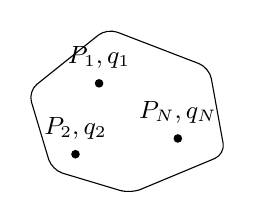
\begin{tikzpicture}\draw[rounded corners](0,0)--(-.3,1)--(.7,1.8)--(2,1.3)--(2.2,.2)--(1,-.3)--cycle;\foreach\x/\y/\l in{.6/1.1/1,.3/.2/2,1.6/.4/N}{\node[pt,label=above:{$P_\l,q_\l$}]at(\x,\y){};}\end{tikzpicture}}
\begin{align*}
E_{p,\mathrm{int}}&=\sum_{i<j}\frac{q_iq_j}{4\pi\eps P_iP_j}
=\frac12\sum_{i\ne j}\frac{q_iq_j}{4\pi\eps P_iP_j}\\
&=\frac12\sum_i\sum_{j\ne i}\frac{q_iq_j}{4\pi\eps P_iP_j}
=\sum_i\frac{q_i}{2}\left[\sum_{j\ne i}\frac{q_j}{4\pi\eps P_iP_j}\right]\\
&=\sum_i\frac{q_i}{2}\underbrace{\left[\sum_{j\ne i}V_{j\to i}\right]}_{V_i}.
\end{align*}
$V_i$ est le potentiel créé en $P_i$ par toutes les charges $j\ne i$.
\begin{result}[2]\[E_{p,\mathrm{int}}=\sum_{i=1}^N\frac12q_iV_i.\]\end{result}
On admet la généralisation pour une distribution volumique :
\begin{result}[2]\[E_{p,\mathrm{int}}=\iiint_\D\frac12\rho(P)V(P)\dd^3\tau.\]\end{result}
\par\textbf{Remarque :}  Ces formules ne sont pas exigibles au programme.
\subsection{Énergie de constitution}
\begin{cadre}\textbf{Définition}\par
On appelle énergie de constitution d'une distribution de charges le travail qu'un opérateur doit fournir à l'ensemble des charges pour les ramener d'une vitesse nulle à l'infini vers leur position finale.
\end{cadre}
État initial : les charges $(q_i)$ sont à l'infini et $\vec v(q_i)=\vec0$.

État final : la distribution est $\D$.
\par\textbf{Remarque :}  L'énergie de constitution peut être positive ou négative.
\begin{center}\begin{tabular}{p{.44\linewidth}|p{.44\linewidth}}
\centering $+q\qquad+q$ &\centering $+q\qquad-q$\tabularnewline
\centering $E_{\mathrm{const}}>0$ &\centering $E_{\mathrm{const}}<0$\tabularnewline
Pour contrer la répulsion électrostatique.&Pour freiner l'attraction électrostatique.
\end{tabular}\end{center}
On cherche à relier $E_{\mathrm{const}}$ et $E_{p,\mathrm{int}}$.

Système : $\D$.

On applique le théorème de l'énergie cinétique entre l'état initial et l'état final :
\[\Delta E_c=W_{\mathrm{ext}}+W_{\mathrm{int}}.\]
La transformation est quasi statique : $v=0$, donc $\Delta E_c=0$. De plus, $W_{\mathrm{ext}}=W_{\mathrm{op}}$. Ainsi,
\[0=W_{\mathrm{op}}+W_{\mathrm{int}},\qquad W_{\mathrm{op}}=-W_{\mathrm{int}}=\Delta E_{p,\mathrm{int}}.\]
\[W_{\mathrm{op}}=E_{p,\mathrm{int},f}-E_{p,\mathrm{int},0}.\]
La référence de l'énergie potentielle est choisie nulle à l'infini : $E_{p,\mathrm{int},0}=0$.
\begin{cadre}\[E_{\mathrm{constitution}}=E_{p,\mathrm{int}}.\]\end{cadre}
% Sources 37--48
\Needspace{65mm}
\section{Exemples de quelques champs électrostatiques}
\subsection{Sphère uniformément chargée}
\titr{Modèle élémentaire du noyau atomique}
\fig{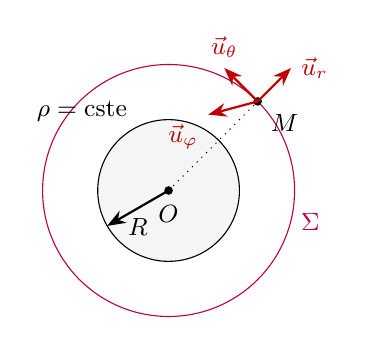
\begin{tikzpicture}\draw[fill=gray!8](0,0)circle(.9);\draw[purple](0,0)circle(1.6);\node[pt,label=below:$O$]at(0,0){};\draw[arr](0,0)--(210:.9)node[midway,below]{$R$};\draw[dotted](0,0)--(45:1.6);\node[pt,label=below right:$M$]at(45:1.6){};\draw[cur](45:1.6)--(45:2.2)node[right]{$\ur$};\draw[cur](45:1.6)--++(135:.6)node[above]{$\ut$};\draw[cur](45:1.6)--++(195:.65)node[below left]{$\uphi$};\node at(-1.1,1){$\rho=\cste$};\node[purple]at(1.8,-.4){$\Sigma$};\end{tikzpicture}}
Dans la base sphérique, $V=V(r,\theta,\varphi)$ et
\[\E=E_r(r,\theta,\varphi)\ur+E_\theta(r,\theta,\varphi)\ut+E_\varphi(r,\theta,\varphi)\uphi.\]
La symétrie sphérique, c'est-à-dire l'invariance par rotation autour de tout axe passant par $O$, donne $V=V(r)$ et des composantes du champ dépendant uniquement de $r$.
Les plans $\Pi_1=(M,\ur,\ut)$ et $\Pi_2=(M,\ur,\uphi)$ sont des plans de symétrie de $\D$, donc de $\E$. Puisque $M$ appartient à ces plans, $\E\in\Pi_1\cap\Pi_2$ et $\E\parallel\ur$.
\begin{cadre}\[\E(M)=E_r(r)\ur.\]\end{cadre}
\par\textbf{Remarque :}  Puisque $V=V(r)$ par symétrie sphérique, on pouvait écrire immédiatement
\[\E=-\grad V(r)=-\frac{\dd V}{\dd r}\ur.\]
Il s'agit d'un problème de haute symétrie : on utilise le théorème de Gauss. La surface de Gauss est une sphère de centre $O$ passant par $M$.
\[\oiint_\Sigma\E\cdot\dS=4\pi r^2E_r(r)=\frac{Q_{\mathrm{int}}}{\eps}.\]
\[\begin{cases}r>R:&Q_{\mathrm{int}}=Q=\rho\dfrac43\pi R^3,\\[3pt]r<R:&Q_{\mathrm{int}}=\rho\dfrac43\pi r^3=Q\dfrac{r^3}{R^3}.\end{cases}\]
D'où
\[\begin{cases}r>R:&E_r(r)=\dfrac{Q}{4\pi\eps r^2},\\[4pt]r<R:&E_r(r)=\dfrac{Qr^3/R^3}{4\pi\eps r^2}=\dfrac{Qr}{4\pi\eps R^3}.\end{cases}\]
\fig{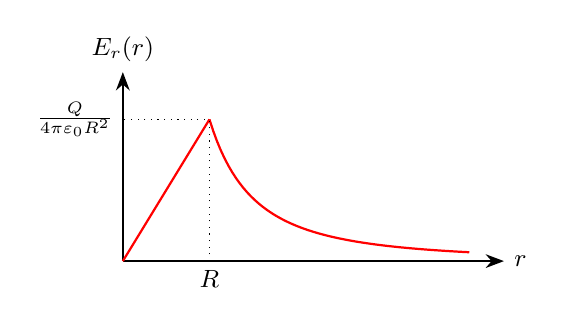
\begin{tikzpicture}[x=1.1cm,y=1.2cm]\draw[arr](0,0)--(4.4,0)node[right]{$r$};\draw[arr](0,0)--(0,2)node[above]{$E_r(r)$};\draw[red,thick](0,0)--(1,1.5);\draw[red,thick,domain=1:4,samples=70]plot(\x,{1.5/\x^2});\draw[dotted](1,0)node[below]{$R$}--(1,1.5)--(0,1.5)node[left]{$\frac{Q}{4\pi\eps R^2}$};\end{tikzpicture}}
\titr{Remarques}
\begin{enumerate}
\item Le champ électrique est continu.
\item Si $\rho$ n'est pas uniforme mais $\rho=\rho(r)$, la symétrie sphérique et le théorème de Gauss sont inchangés. Pour $r>R$, $Q_{\mathrm{int}}=Q$, avec
\[Q=\iiint_{\mathcal V}\rho(r')\dd^3\tau=\int_0^R\rho(r')4\pi r'^2\dd r'.\]
Pour $r<R$, $Q_{\mathrm{int}}=\int_0^r\rho(u)4\pi u^2\dd u$.
\item \begin{minipage}[t]{\linewidth}\vspace{0pt}\begin{result}[5]Pour une distribution sphérique de charges, uniforme ou non, avec $\rho=\rho(r)$, le champ à l'extérieur de la distribution est le même que celui créé par une charge ponctuelle égale à la charge totale de la distribution.\end{result}\end{minipage}
\item \textbf{Application numérique pour l'atome d'hydrogène}
\fig{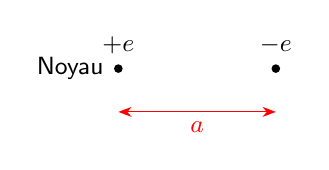
\begin{tikzpicture}\node[pt,label=above:$+e$,label=left:Noyau]at(0,0){};\node[pt,label=above:$-e$]at(2,0){};\draw[<->,red](0,-.55)--(2,-.55)node[midway,below]{$a$};\end{tikzpicture}}
\[E_{\mathrm{noyau}\to e^-}=\frac{e}{4\pi\eps a^2},\qquad a\simeq1\ \text{\AA}.\]
\begin{cadre}\[E\sim1\times10^{11}\ \mathrm{V\,m^{-1}}.\]\end{cadre}
Pour ioniser un atome d'hydrogène, il faut fournir un champ d'au moins $10^{11}\ \mathrm{V\,m^{-1}}$, difficile à obtenir. Le champ d'ionisation de l'air est $1\times10^6\ \mathrm{V\,m^{-1}}$ dans les conditions usuelles de température et d'humidité ; il est relativement facile à obtenir, par exemple avec une machine de Wimshurst.
\end{enumerate}
\titr{Calcul de $V$}
\[\begin{cases}r>R:&E_r(r)=\dfrac Q{4\pi\eps r^2}=-\dfrac{\dd V}{\dd r},\\[4pt]r<R:&E_r(r)=\dfrac{Qr}{4\pi\eps R^3}=-\dfrac{\dd V}{\dd r}.\end{cases}\]
\[\begin{cases}r>R:&V(r)=\dfrac Q{4\pi\eps r}+C_1,\\[4pt]r<R:&V(r)=-\dfrac{Qr^2}{8\pi\eps R^3}+C_2.\end{cases}\]
La référence $V\to0$ lorsque $r\to+\infty$ donne $C_1=0$. Par continuité, $V(R^-)=V(R^+)$.
\begin{cadre}\[\begin{cases}r>R:&V(r)=\dfrac Q{4\pi\eps r},\\[4pt]r<R:&V(r)=\dfrac Q{8\pi\eps R^3}(3R^2-r^2).\end{cases}\]\end{cadre}
\fig{\begin{tikzpicture}[x=1.1cm,y=1cm]\draw[arr](0,0)--(4.3,0)node[right]{$r$};\draw[arr](0,0)--(0,2.7)node[above]{$V(r)$};\draw[red,thick,domain=0:1]plot(\x,{2.4-.8*\x^2});\draw[red,thick,domain=1:4,samples=70]plot(\x,{1.6/\x});\draw[dotted](1,0)node[below]{$R$}--(1,1.6)--(0,1.6);\draw[<->,purple](-.4,2.4)--(.4,2.4);\end{tikzpicture}}
\begin{exemple}\examtitle{Énergie de constitution d'un noyau atomique}
Dans la réalité, les interactions fortes sont responsables de la stabilité : elles l'emportent sur les interactions électrostatiques. Ici, on s'intéresse à l'énergie de constitution électrostatique, avec $E_{\mathrm{const}}>0$ : le noyau est instable.
Trois méthodes sont possibles.
\titr{1) Analyse dimensionnelle}
Les grandeurs physiques sont $Q$, $R$ et $\eps$. Une grandeur homogène à une énergie s'écrit
\begin{cadre}\[E_{\mathrm{const}}=\alpha\frac{Q^2}{R(4\pi\eps)},\]\end{cadre}
où $\alpha$ est une constante sans dimension.
\titr{2) Par l'énergie potentielle d'interaction}
\par\textbf{Remarque :}  Cette méthode est hors programme.
\[E_{p,\mathrm{int}}=E_{\mathrm{const}}=\frac12\iiint_\D\rho(P)V(P)\dd^3\tau.\]
\[E_{\mathrm{const}}=\frac12\int_0^R\rho\left[-\frac Q{8\pi\eps R^3}(r^2-3R^2)\right]4\pi r^2\dd r.\]
\begin{cadre}\[E_{\mathrm{const}}=\frac35\frac{Q^2}{4\pi\eps R}.\]\end{cadre}
\titr{3) Par définition de l'énergie de constitution}
Cette méthode est exigible. On constitue le noyau étape par étape, de manière quasi statique.
\fig{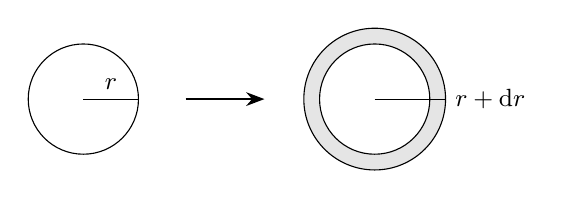
\begin{tikzpicture}\draw(0,0)circle(.7);\draw(0,0)--(.7,0)node[midway,above]{$r$};\draw[arr](1.3,0)--(2.3,0);\draw[fill=gray!20](3.7,0)circle(.9);\draw[fill=white](3.7,0)circle(.7);\draw(3.7,0)--(4.6,0)node[right]{$r+\dd r$};\end{tikzpicture}}
On ramène de l'infini, de manière quasi statique, la charge $\dd q=\rho4\pi r^2\dd r$.

Système : la charge $\dd q=\rho4\pi r^2\dd r$.

On applique le théorème de l'énergie cinétique entre l'état initial, où la charge est à l'infini, et l'état final, où elle est ramenée sur la distribution en $r+\dd r$.
\begin{align*}
\dd E_c=0&=\delta W_{\mathrm{op}}+\delta W_{\mathrm{elec}}
=\delta W_{\mathrm{op}}-\dd E_{p,\mathrm{elec}},\\
\delta W_{\mathrm{op}}&=\dd E_{p,\mathrm{elec}}=\dd q(V_f-V_0)\\
&=(4\pi r^2\dd r\,\rho)\left(\frac1{4\pi\eps r}\frac{Qr^3}{R^3}-0\right)
=\frac{r^4\rho Q}{\eps R^3}\dd r.
\end{align*}
Le potentiel utilisé est celui créé par une distribution sphérique à l'extérieur de celle-ci.
\[W_{\mathrm{op}}=\int_0^R\delta W_{\mathrm{op}}=\int_0^R\frac{r^4\rho Q}{\eps R^3}\dd r.\]
\begin{cadre}\[W_{\mathrm{op}}=\frac35\frac{Q^2}{4\pi\eps R}.\]\end{cadre}
\textbf{Application numérique pour l'atome d'hélium}
\[Q=Ze=2e,\qquad E_{\mathrm{const}}=6\ \mathrm{MeV}>0.\]
\par\textbf{Remarque :}  On trouve, par hasard, les bons ordres de grandeur correspondant à l'énergie nécessaire pour casser un noyau. Or $E_{\mathrm{const}}>0$ : le noyau est instable d'un point de vue purement électrostatique.
\end{exemple}
\titr{Sphère chargée surfaciquement}
\fig{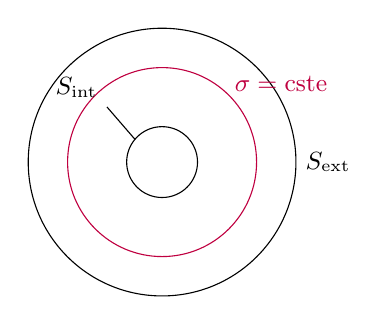
\begin{tikzpicture}\draw(0,0)circle(.45);\draw[purple](0,0)circle(1.2);\draw(0,0)circle(1.7);\draw[thin](140:.45)--(-.7,.7);\node[above left]at(-.7,.7){$S_{\mathrm{int}}$};\node[right]at(1.7,0){$S_{\mathrm{ext}}$};\node[purple,right]at(.8,1){$\sigma=\cste$};\end{tikzpicture}}
Les symétries sont identiques. Le théorème de Gauss donne
\[4\pi r^2E_r(r)=\frac{Q_{\mathrm{int}}}{\eps}.\]
\[\begin{cases}r<R:&Q_{\mathrm{int}}=0,\quad E_r(r)=0,\\[4pt]r>R:&Q_{\mathrm{int}}=Q,\quad E_r(r)=\dfrac Q{4\pi\eps r^2}.\end{cases}\]
\fig{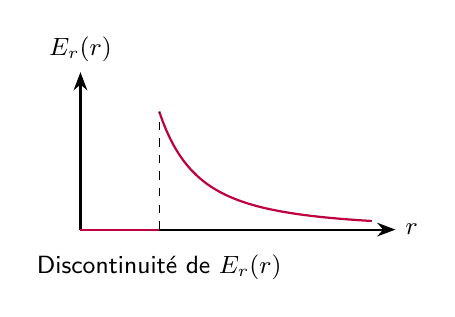
\begin{tikzpicture}\draw[arr](0,0)--(4,0)node[right]{$r$};\draw[arr](0,0)--(0,2)node[above]{$E_r(r)$};\draw[purple,thick](0,0)--(1,0);\draw[purple,thick,domain=1:3.7,samples=60]plot(\x,{1.5/\x^2});\draw[dashed](1,0)--(1,1.5);\node[below,align=center]at(1,-.2){Discontinuité de $E_r(r)$};\end{tikzpicture}}
% Sources 48--55
\subsection{Cylindre infini uniformément chargé}
\fig{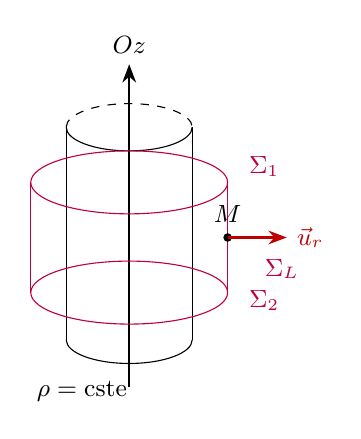
\begin{tikzpicture}\draw[dashed](-.8,1.4)arc(180:0:.8 and .3);\draw(-.8,1.4)arc(180:360:.8 and .3);\draw(-.8,1.4)--(-.8,-1.3)(.8,1.4)--(.8,-1.3);\draw(-.8,-1.3)arc(180:360:.8 and .3);\draw[arr](0,-1.9)--(0,2.2)node[above]{$Oz$};\draw[purple](-1.25,.7)ellipse(0 and 0);\draw[purple](0,.7)ellipse(1.25 and .4);\draw[purple](-1.25,.7)--(-1.25,-.7)(1.25,.7)--(1.25,-.7);\draw[purple](0,-.7)ellipse(1.25 and .4);\node[purple,right]at(1.4,.9){$\Sigma_1$};\node[purple,right]at(1.4,-.8){$\Sigma_2$};\node[purple,right]at(1.6,-.4){$\Sigma_L$};\node[pt,label=above:$M$]at(1.25,0){};\draw[cur](1.25,0)--(2,0)node[right]{$\ur$};\node[below]at(-.6,-1.7){$\rho=\cste$};\end{tikzpicture}}
Dans la base cylindrique,
\[V=V(r,\theta,z),\qquad\E=E_r(r,\theta,z)\ur+E_\theta(r,\theta,z)\ut+E_z(r,\theta,z)\uz.\]
L'invariance par translation parallèle à $Oz$ et par rotation autour de $Oz$ donne une symétrie cylindrique : $V=V(r)$ et les composantes de $\E$ ne dépendent que de $r$.
Puisque $V=V(r)$, $\E=E_r(r)\ur$.
Les plans $(M,\ur,\ut)$ et $(M,\ur,\uz)$ sont des plans de symétrie de $\D$, donc de $\E$ : $\E\parallel\ur$.
La surface de Gauss est un cylindre de rayon $r$ et de hauteur $h$.
\begin{align*}\oiint_\Sigma\E\cdot\dS
&=\iint_{\Sigma_1}\E\cdot\dS+\iint_{\Sigma_2}\E\cdot\dS+\iint_{\Sigma_L}\E\cdot\dS\\
&=0+0+\iint_{\Sigma_L}E_r(r)2\pi r\dd h.
\end{align*}
\[\frac{Q_{\mathrm{int}}}{\eps}=E_r(r)2\pi rh.\]
Pour $r>R$, $Q_{\mathrm{int}}=\rho\pi R^2h$ ; pour $r<R$, $Q_{\mathrm{int}}=\rho\pi r^2h$.
\[r>R:\quad2\pi rhE_r(r)=\frac{\rho\pi R^2h}{\eps};\qquad
r<R:\quad2\pi rhE_r(r)=\frac{\rho\pi r^2h}{\eps}.\]
\begin{cadre}\[r>R:\ E_r(r)=\frac{\rho R^2}{2\eps r},\qquad r<R:\ E_r(r)=\frac{\rho r}{2\eps}.\]\end{cadre}
\fig{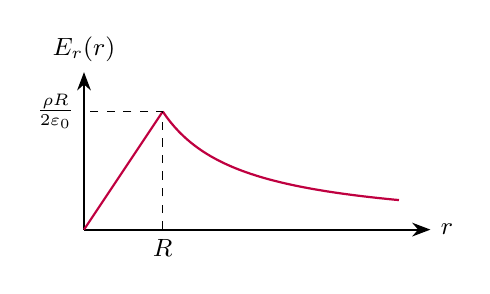
\begin{tikzpicture}\draw[arr](0,0)--(4.4,0)node[right]{$r$};\draw[arr](0,0)--(0,2)node[above]{$E_r(r)$};\draw[purple,thick](0,0)--(1,1.5);\draw[purple,thick,domain=1:4,samples=60]plot(\x,{1.5/\x});\draw[dashed](1,0)node[below]{$R$}--(1,1.5)--(0,1.5)node[left]{$\frac{\rho R}{2\eps}$};\end{tikzpicture}}
\[E_r(r)=-\frac{\dd V}{\dd r},\qquad
\begin{cases}r>R:&V(r)=-\dfrac{\rho R^2}{2\eps}\ln r+C_1,\\[3pt]r<R:&V(r)=-\dfrac{\rho r^2}{4\eps}+C_2.\end{cases}\]
Ici, le choix $V\to0$ lorsque $r\to+\infty$ n'est pas possible : $V(r)$ diverge car le cylindre est infini. On peut par exemple poser $V(0)=0$, d'où $C_2=0$, et déduire $C_1$ par continuité de $V$.
\titr{Remarques}
\titr{1) Distribution non uniforme : $\rho=\rho(r)$}
La symétrie cylindrique, les symétries et le cylindre de Gauss restent identiques.
\[2\pi rhE_r(r)=\frac{Q_{\mathrm{int}}}{\eps}.\]
\[r>R:\quad Q_{\mathrm{int}}=\int_0^R\rho(r')2\pi r'\dd r'\,h;\qquad
r<R:\quad Q_{\mathrm{int}}=\int_0^r\rho(r')2\pi r'\dd r'\,h.\]
\fig{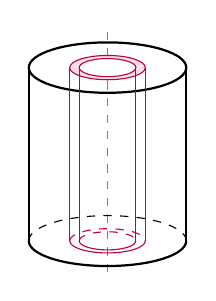
\begin{tikzpicture}\draw[gray,dashed](0,-1.5)--(0,1.6);
\draw[thick](0,1.1)ellipse(1 and .32);\draw[thick](-1,1.1)--(-1,-1.1)(1,1.1)--(1,-1.1);\draw[thick](-1,-1.1)arc(180:360:1 and .32);\draw[dashed](-1,-1.1)arc(180:0:1 and .32);
\draw[purple,fill=purple!12](0,1.1)ellipse(.48 and .154);\draw[purple,fill=white](0,1.1)ellipse(.36 and .115);
\foreach\r/\h in{.48/.154,.36/.115}{\draw[purple](-\r,1.1)--(-\r,-1.1)(\r,1.1)--(\r,-1.1);\draw[purple](-\r,-1.1)arc(180:360:\r cm and \h cm);\draw[purple,dashed](-\r,-1.1)arc(180:0:\r cm and \h cm);}
\end{tikzpicture}}
\titr{2) Distribution surfacique}
\fig{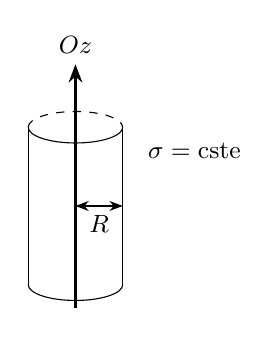
\begin{tikzpicture}\draw[dashed](-.6,1)arc(180:0:.6 and .2);\draw(-.6,1)arc(180:360:.6 and .2);\draw(-.6,1)--(-.6,-1)(.6,1)--(.6,-1);\draw(-.6,-1)arc(180:360:.6 and .2);\draw[arr](0,-1.3)--(0,1.8)node[above]{$Oz$};\draw[<->](0,0)--(.6,0)node[midway,below]{$R$};\node[right]at(.8,.7){$\sigma=\cste$};\end{tikzpicture}}
Les symétries et la surface de Gauss sont identiques.
\[2\pi rhE_r(r)=\frac{Q_{\mathrm{int}}}{\eps}.\]
\[\begin{cases}r>R:&Q_{\mathrm{int}}=\sigma2\pi Rh,\quad E_r=\dfrac{\sigma2\pi Rh}{\eps2\pi rh}=\dfrac{\sigma R}{\eps r},\\[4pt]r<R:&Q_{\mathrm{int}}=0,\quad E_r=0.\end{cases}\]
\fig{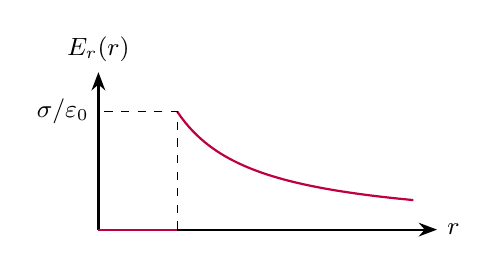
\begin{tikzpicture}\draw[arr](0,0)--(4.3,0)node[right]{$r$};\draw[arr](0,0)--(0,2)node[above]{$E_r(r)$};\draw[purple,thick](0,0)--(1,0);\draw[purple,thick,domain=1:4,samples=60]plot(\x,{1.5/\x});\draw[dashed](1,0)--(1,1.5)--(0,1.5)node[left]{$\sigma/\eps$};\end{tikzpicture}}

\titr{3) Limite $R\to0$ : distribution linéique}
On obtient un fil. Les symétries et la surface de Gauss sont identiques.
\fig{\begin{tikzpicture}\draw[purple](0,-1)--(0,1.2)node[above]{$\lambda=\cste$};\node[pt,label=right:$M$]at(1,0){};\end{tikzpicture}}
\[2\pi rhE_r(r)=\frac{Q_{\mathrm{int}}}{\eps}=\frac{\lambda h}{\eps}.\]
\begin{cadre}\[E_r(r)=\frac\lambda{2\pi\eps r},\qquad V(r)=-\frac\lambda{2\pi\eps}\ln r.\]\end{cadre}
% Sources 55--59
\subsection{Plan infini uniformément chargé}
\fig{\begin{tikzpicture}\draw[fill=gray!5](-3,-.65)--(2.5,-.65)--(3.4,.8)--(-2.1,.8)--cycle;
\node at(-2.1,.5){$\sigma=\cste$};
\draw[cur](-1.3,-.05)--(-.55,-.05)node[right]{$x$};\draw[cur](-1.3,-.05)--(-1.3,.9)node[above]{$z$};\draw[cur](-1.3,-.05)--(-.95,.55)node[right]{$y$};\node[below left]at(-1.3,-.05){$O$};
\draw[purple](1,1.25)ellipse(.7 and .24);\draw[purple](1,-1.25)ellipse(.7 and .24);\draw[purple](.3,-1.25)--(.3,1.25)(1.7,-1.25)--(1.7,1.25);
\draw[purple,thin](1.5,1.4)--(2.25,1.8)node[right]{$\Sigma_h$};
\draw[purple,thin](1.7,-.4)--(2.25,-.65)node[right]{$\Sigma_L$};
\draw[purple,thin](1.5,-1.4)--(2.25,-1.75)node[right]{$\Sigma_{-h}$};
\node[pt,label=above left:$M$]at(1,1.25){};
\draw[<->](3.5,0)--(3.5,1.25)node[midway,right]{$h$};\draw[<->](3.5,-1.25)--(3.5,0)node[midway,right]{$h$};\end{tikzpicture}}
Initialement, $V(M)=V(x,y,z)$ et
\[\E(M)=E_x(x,y,z)\ux+E_y(x,y,z)\uy+E_z(x,y,z)\uz.\]
Les invariances par translation parallèle à $Ox$ et à $Oy$ donnent $V=V(z)$ et $\E=\E(z)$. Comme $\E=-\grad V$,
\begin{cadre}\[\E(z)=E_z(z)\uz.\]\end{cadre}
Les plans $\Pi_1=(M,\ux,\uz)$ et $\Pi_2=(M,\uy,\uz)$ sont des plans de symétrie de $\E$. Ainsi, $\E\in\Pi_1\cap\Pi_2$, donc $\E\parallel\uz$.
Le plan $Oxy$ est un plan de symétrie de $\D$ et de $\E$, d'où $E_z(-z)=-E_z(z)$.
\fig{\begin{tikzpicture}\draw(-2,0)--(2,0)node[right]{$\sigma$};\draw[arr](0,-1.2)--(0,1.3);\draw[purple](.6,-.7)rectangle(1,.7);\node[pt,label=right:$M$]at(.8,.7){};\node[pt,label=right:$M'$]at(.8,-.7){};\draw[cur](.8,.7)--(.8,1.3);\draw[cur](.8,-.7)--(.8,-1.3);\end{tikzpicture}}
\begin{align*}\oiint_\Sigma\E\cdot\dS
&=\iint_{\Sigma_h}\E\cdot\dS+\iint_{\Sigma_{-h}}\E\cdot\dS+\iint_{\Sigma_L}\E\cdot\dS\\
&=2\iint_{\Sigma_h}\E\cdot\dS+0.
\end{align*}
Les deux premiers termes sont égaux par symétrie ; le dernier est nul car $\E\perp\dS$ sur la surface latérale. Pour $z>0$,
\[\frac{Q_{\mathrm{int}}}{\eps}=2E_z(z)S,\qquad\frac{\sigma S}{\eps}=2E_z(z)S.\]
\begin{result}\[E_z(z)=\frac\sigma{2\eps}\quad\text{pour }z>0.\]\end{result}
\fig{\begin{tikzpicture}\draw[arr](-2,0)--(2.2,0)node[right]{$z$};\draw[arr](0,-1.3)--(0,1.5)node[above]{$E_z(z)$};\draw[red,thick](-1.8,-.8)--(0,-.8)(0,.8)--(1.8,.8);\node[above left]at(0,.8){$\sigma/(2\eps)$};\node[below right]at(0,-.8){$-\sigma/(2\eps)$};\end{tikzpicture}\hspace{1cm}\begin{tikzpicture}\draw(-1.8,0)--(1.8,0);\foreach\x in{-1.5,-1,...,1.5}{\draw[el](\x,.2)--(\x,1);\draw[el](\x,-.2)--(\x,-1);}\end{tikzpicture}}
Le champ est uniforme au-dessus et au-dessous du plan.
\[E_z(z)=-\frac{\dd V}{\dd z},\qquad
\begin{cases}z>0:&V(z)=-\dfrac{\sigma z}{2\eps}+C_1,\\[3pt]z<0:&V(z)=\dfrac{\sigma z}{2\eps}+C_2.\end{cases}\]
En posant $V(0)=0$ et par continuité, $V(0^+)=V(0^-)=0$, donc $C_1=C_2=0$.
\fig{\begin{tikzpicture}\draw[arr](-2,0)--(2.2,0)node[right]{$z$};\draw[arr](0,-1.8)--(0,.6)node[above]{$V(z)$};\draw[red,thick](-1.8,-1.5)--(0,0)--(1.8,-1.5);\end{tikzpicture}}
% Sources 59--71
\subsection{Condensateur plan}
\subsubsection{Conducteurs}
\begin{cadre}Un conducteur est un matériau qui contient des charges libres de se déplacer.\end{cadre}
Exemple : le cuivre.

\begin{cadre}Un milieu diélectrique est un milieu isolant.\end{cadre}
\begin{cadre}Un conducteur en équilibre électrostatique est un conducteur où il n'y a pas de courant : il n'y a pas de mouvement de l'ensemble des charges.\end{cadre}
\begin{cadre}\[\text{Conducteur en équilibre électrostatique}\quad\Longleftrightarrow\quad\E(M)=\vec0,\quad V=\cste.\]\end{cadre}
Puisque $\divg\E=\rho/\eps$, on a $\rho=0$.
\fig{\begin{tikzpicture}\draw[rounded corners](-1,-.8)--(-1.4,.4)--(-.4,1)--(.6,.7)--(1.3,0)--(.6,-1)--cycle;\node[red,align=center]at(0,0){$\E=\vec0$\\$\rho=0$\\$V=\cste$};\node[right,align=left]at(1.7,.3){Conducteur en équilibre\\électrostatique};\draw[el](.2,-.95)--(.2,-1.65)node[below,align=center]{$\sigma(P)$ : possibilité de charges en surface};\end{tikzpicture}}
\titr{Deux applications}
\textbf{Effet de pointe}
\fig{\begin{tikzpicture}\begin{scope}[xshift=-.8cm]
\begin{scope}\clip(0,-1.6)rectangle(2.65,1.6);
\draw[fill=gray!8,thick](0,0)ellipse(2 and .48);\node at(.8,0){$V=\cste$};
\foreach\a/\b in{2.13/.875,2.28/1.195,2.48/1.541}{\draw[green!50!black](0,0)ellipse(\a cm and \b cm);}
\foreach\v in{-80,-55,-30,-15,0,15,30,55,80}{
\draw[purple,thick,postaction={decorate},decoration={markings,mark=at position .62 with {\arrow{Stealth}}},domain=.73:.2449,variable=\u,samples=35]plot({1.941*cosh(\u)*cos(\v)},{1.941*sinh(\u)*sin(\v)});}
\end{scope}\node[green!50!black,above]at(1.2,1.7){Surfaces équipotentielles};
\node[below,align=center]at(1.2,-1.85){Resserrement des lignes de champ à la pointe : $\|\E\|$ augmente};
\end{scope}\end{tikzpicture}}
\begin{exemple}\examtitle{Tourniquet électrostatique}
\fig{\begin{tikzpicture}\draw[thick](-1,.7)--(-1,0)--(1,0)--(1,-.7)(-.7,-1)--(0,-1)--(0,1)--(.7,1);
\foreach\x/\y/\a in{-1/.7/90,1/-.7/-90,-.7/-1/180,.7/1/0}{\draw[el](\x,\y)--++(\a:.55);}
\node[purple,above]at(-1,1.3){$e^-$};\node[purple,below]at(1,-1.3){$e^-$};\node[purple,left]at(-1.3,-1){$e^-$};\node[purple,right]at(1.3,1){$e^-$};
\foreach\x/\y/\a in{-1/.7/90,1/-.7/-90,-.7/-1/180,.7/1/0}{
\begin{scope}[shift={(\x,\y)},rotate=\a]
\foreach\u/\v in{-.12/-.18,-.12/.18,-.3/.18}{\node[red,font=\tiny,inner sep=0pt]at(\u,\v){$-$};}\end{scope}}
\end{tikzpicture}}
Le champ est plus intense sur les pointes. Les électrons sont éjectés, ce qui entraîne la rotation du tourniquet.
\end{exemple}
\textbf{Cage de Faraday}
\fig{\begin{tikzpicture}\draw[fill=gray!12](0,0)circle(1.1);\draw[fill=white](0,0)circle(.85);\node[purple]at(0,0){Intérieur};\node[purple,right]at(1.3,0){Extérieur};\node[above]at(0,1.1){Conducteur};\draw[thin](-.6,-.6)--(-1.1,-1.3)node[below left]{$\Sigma_{\mathrm{int}}$};\end{tikzpicture}}
L'intérieur est électriquement isolé de l'extérieur. À l'intérieur, $\Delta V=0$, avec la condition limite $V_{\Sigma_{\mathrm{int}}}=V_1$. Ainsi, à l'intérieur, $V=V_1$ et $\E=\vec0$, peu importe ce qui se passe à l'extérieur : il y a protection de l'extérieur.
\subsubsection{Définition d'un condensateur}
\begin{cadre}Un condensateur est un ensemble de deux conducteurs en influence totale : toutes les lignes de champ partent d'un conducteur vers l'autre conducteur.\end{cadre}
\fig{\begin{tikzpicture}\draw[fill=gray!12](0,0)ellipse(2 and 1.5);\draw[fill=white](0,0)ellipse(1.8 and 1.3);\draw[fill=gray!15](0,0)ellipse(.5 and .4);\node at(0,0){$C_1$};\node[below]at(0,-.45){$V_1$};\draw[thin](-1.4,-.96)--(-2.1,-1.55)node[left]{$V_2=\cste$};\foreach\a in{20,65,115,160,205,250,295,340}{\draw[cur]({.55*cos(\a)},{.45*sin(\a)})--({1.7*cos(\a)},{1.2*sin(\a)});}\node[purple]at(.8,.5){$\sigma_1$};\draw[purple,thin](1.55,.66)--(2.3,.25)node[right]{$\sigma_2$};\node[purple]at(2.2,.8){$\sigma_3$};\end{tikzpicture}}
Les deux conducteurs constituent les deux armatures du condensateur.
\begin{exemple}\examtitle{Exemples de condensateurs}
\fig{\begin{tikzpicture}\draw[fill=gray!20](0,0)circle(1);\draw[fill=white](0,0)circle(.85);\draw[fill=gray!20](0,0)circle(.3);\node at(0,0){$C_1$};\foreach\a in{0,60,...,300}{\draw[cur](\a:.35)--(\a:.8);}\node[below]at(0,-1.2){Sphérique};\begin{scope}[xshift=4cm]\draw[fill=gray!15](0,-.5)ellipse(1 and .4);\draw[fill=white](0,-.5)ellipse(.8 and .3);\draw(-1,-.5)--(-1,.7)(1,-.5)--(1,.7);\draw[fill=gray!15](0,.7)ellipse(1 and .4);\draw[fill=white](0,.7)ellipse(.8 and .3);\draw[thick](0,-.5)--(0,.7);\foreach\a in{20,100,180,260}{\draw[cur](0,.7)--({.75*cos(\a)},{.7+.27*sin(\a)});}\node[below]at(0,-1.2){Cylindrique};\end{scope}\end{tikzpicture}}
\fig{\begin{tikzpicture}\begin{scope}
\draw[fill=gray!5](0,0)--(2.4,0)--(2.8,.45)--(.4,.45)--cycle;
\draw[fill=gray!5](0,0)--(1.697,1.697)--(2.097,2.147)--(.4,.45)--cycle;
\begin{scope}[shift={(.2,.225)}]\foreach\r in{.65,1.15,1.65,2.15}{\draw[cur] (\r,0)arc(0:45:\r);}\end{scope}
\node[below]at(1.3,-.25){Diédrique};\end{scope}
\begin{scope}[xshift=6cm]
\draw[fill=gray!5](-2,-.15)--(2,-.15)--(2.4,.35)--(-1.6,.35)--cycle;
\draw[fill=gray!12](0,0)--(-.65,1.55)arc(180:0:.65 and .2)--cycle;
\draw(0,1.55)ellipse(.65 and .2);
\foreach\r in{.65,1.05,1.45}{\draw[cur](\r,0)arc(0:67.25:\r);\draw[cur](-\r,0)arc(180:112.75:\r);}
\node[below]at(0,-.4){Conique};\end{scope}\end{tikzpicture}}
\end{exemple}
\fig{\begin{tikzpicture}\draw[fill=gray!12](0,0)ellipse(2 and 1.5);\draw[fill=white](0,0)ellipse(1.8 and 1.3);\draw[fill=gray!15](0,0)ellipse(.5 and .4);\node at(0,0){$C_1$};\node[below]at(0,-.45){$V_1$};\draw[thin](-1.4,-.96)--(-2.1,-1.55)node[left]{$V_2=\cste$};\foreach\a in{20,65,115,160,205,250,295,340}{\draw[cur]({.55*cos(\a)},{.45*sin(\a)})--({1.7*cos(\a)},{1.2*sin(\a)});}\node[purple]at(.8,.5){$\sigma_1$};\draw[purple,thin](1.55,.66)--(2.3,.25)node[right]{$\sigma_2$};\node[purple]at(2.2,.8){$\sigma_3$};\draw[purple,dashed](0,0)ellipse(1.9 and 1.4);\draw[el](1.35,1)--(2.3,1.7)node[right]{$\Sigma$};\end{tikzpicture}}
Les deux armatures sont deux conducteurs en influence totale. On choisit une surface de Gauss fermée $\Sigma$ dans le conducteur extérieur :
\[\oiint_\Sigma\E\cdot\dS=\frac{Q_{\mathrm{int}}}{\eps}=\frac{Q_1+Q_2}{\eps}.\]
Or $\E=\vec0$ dans le conducteur en équilibre électrostatique. Donc $0=Q_1+Q_2$.
\begin{cadre}\[Q_2=-Q_1.\]\end{cadre}
\titr{Capacité d'un condensateur}
\begin{cadre}\[C=\frac{Q_1}{V_1-V_2}.\]\end{cadre}
\begin{itemize}\item $C>0$.\item La capacité ne dépend que de la géométrie du condensateur et du milieu de l'espace interarmatures.\end{itemize}
\subsubsection{Modèle du condensateur plan}
\begin{cadre}On appelle condensateur plan un condensateur constitué de deux armatures planes, parallèles, de même forme, de même surface et de même nature, espacées d'une distance $e$.
\begin{itemize}\item On suppose $e\ll\text{dimensions des plaques}$.\item Les plaques sont considérées comme infinies.\item Les effets de bord sont négligés.\end{itemize}\end{cadre}
\fig{\begin{tikzpicture}\draw[thick](0,-1)--(0,1)(1,-1)--(1,1);\draw(-1.5,0)--(0,0)(1,0)--(2.5,0);\node[red,above]at(0,1){$+\sigma$};\node[green!50!black,above]at(1,1){$-\sigma$};\draw[<->](0,-1.3)--(1,-1.3)node[midway,below]{$e$};\node[right]at(1.5,-.7){Surface $S$};\end{tikzpicture}}
\titr{Théorème de superposition}
Pour un plan infini, le champ a pour norme $\sigma/(2\eps)$.
\fig{\begin{tikzpicture}\draw[thick](0,-1.2)--(0,1.2)(1,-1.2)--(1,1.2);\node[red,above]at(0,1.2){$+\sigma$};\node[green!50!black,above]at(1,1.2){$-\sigma$};\foreach\y in{-.9,-.3,.3,.9}{\draw[cur](-.3,\y)--(-1,\y);\draw[cur](.2,\y)--(.8,\y);\draw[cur](1.2,\y)--(1.9,\y);\draw[mag,densely dashed](-1,\y+.13)--(-.3,\y+.13);\draw[mag,densely dashed](.2,\y+.13)--(.8,\y+.13);\draw[mag,densely dashed](1.9,\y+.13)--(1.2,\y+.13);}\node[below]at(-.7,-1.4){$\vec0$};\node[below]at(.5,-1.4){$\frac\sigma\eps\uz$};\node[below]at(1.6,-1.4){$\vec0$};\end{tikzpicture}\hspace{1cm}\begin{tikzpicture}\draw[arr](-1,0)--(3,0)node[right]{$z$};\draw[arr](0,-.3)--(0,1.6)node[above]{$E_z$};\draw[purple,thick](-.8,0)--(0,0)--(0,1)--(1.4,1)--(1.4,0)--(2.7,0);\node[left]at(0,1){$\sigma/\eps$};\node[below]at(1.4,0){$e$};\end{tikzpicture}}
\begin{result}Le champ est uniforme dans l'espace interarmatures :\[\E=\frac\sigma\eps\uz.\]\end{result}
Puisque $\E=-\grad V$,
\[z<0:\quad V(z)=V_1;\qquad z>e:\quad V(z)=V_2.\]
Pour $0<z<e$,
\[V(z)=-\frac\sigma\eps z+\cste=-\frac{\sigma z}{\eps}+V_1.\]
\fig{\begin{tikzpicture}\draw[arr](-1.2,0)--(3.3,0)node[right]{$z$};\draw[arr](0,-.2)--(0,2.2)node[above]{$V(z)$};\draw[red,thick](-1,1.8)--(0,1.8)--(1.6,1)--(3,1);\draw[dashed](0,1)node[left]{$V_2$}--(1.6,1)--(1.6,0)node[below]{$e$};\node[left]at(0,1.8){$V_1$};\end{tikzpicture}}
\begin{minipage}{\linewidth}
Donc $V_2=-\sigma e/\eps+V_1$.
\begin{cadre}\[V_1-V_2=\frac{\sigma e}{\eps}.\]\end{cadre}
Comme $V_1-V_2=Q_1e/(S\eps)$,
\begin{result}\[C=\frac{\eps S}{e}.\]\end{result}
\end{minipage}
\titr{Énergie électromagnétique stockée par un condensateur}
\fig{\begin{tikzpicture}\draw(0,-.7)--(0,.7)(.7,-.7)--(.7,.7);\foreach\y in{-.5,0,.5}{\draw[cur](.08,\y)--(.62,\y);}\node[left]at(-.2,0){$\E=\vec0$};\node[right]at(.9,0){$\E=\vec0$};\end{tikzpicture}}
\begin{cadre}\[\E=\frac\sigma\eps\uz=\frac Q{\eps S}\uz.\]\end{cadre}
\begin{result}\[\E=\frac{V_1-V_2}{e}\uz.\]\end{result}
Rappel : la densité volumique d'énergie électromagnétique vaut
\[u_{\mathrm{em}}=\frac12\eps E^2+\underbrace{\frac{B^2}{2\mu_0}}_{=0}.\]
Donc, puisque le champ est uniforme,
\begin{align*}U_{\mathrm{em}}&=\iiint_{\text{condensateur}}\frac12\eps E^2\dd^3\tau=\frac12\eps E^2Se\\
&=\frac12\eps\left(\frac{V_1-V_2}{e}\right)^2Se
=\frac12\underbrace{\frac{\eps S}{e}}_{C}\underbrace{(V_1-V_2)^2}_{u^2}.
\end{align*}
\begin{cadre}\[U_{\mathrm{em}}=\frac12Cu^2=\frac12\frac{Q^2}{C}.\]\end{cadre}
L'énergie stockée dans un condensateur est l'énergie contenue dans le champ électrique du condensateur.
\titr{Remarques}
\[C=\frac{\eps S}{e}.\]
Unité : farad.
Dans les vrais condensateurs, on met un milieu diélectrique entre les armatures. Sa permittivité diélectrique relative est $\varepsilon_r>1$.
\begin{cadre}\[C=\eps\varepsilon_r\frac Se.\]\end{cadre}
Exemples : céramique, papier ; pour le mica, $\varepsilon_r=7$.
% Sources 71--77 : textes photographies integralement retranscrits.
\section{Analogie avec le champ gravitationnel}
\subsection{Champ et potentiel gravitationnels créés par une masse ponctuelle}
Deux points matériels de masses $m$ et $m'$ sont respectivement placés aux points $O$ et $M$. La masse $m$ exerce sur la masse $m'$ une force $\vec F$ dite de gravitation dont l'expression est donnée par la loi de Newton :
\begin{cadre}\[\vec F=-G\frac{mm'}{r^2}\ur.\]\end{cadre}
\fig{\begin{tikzpicture}\node[pt,label=below:{$O,m$}]at(0,0){};\node[pt,label=below:{$M,m'$}]at(2,1){};\draw[dashed](0,0)--(2,1)node[midway,above]{$r$};\draw[arr](2,1)--(2.8,1.4)node[right]{$\ur$};\end{tikzpicture}}
On note $OM=r$ et $\ur=\overrightarrow{OM}/r$. $G$ est une constante universelle positive dont la valeur dépend des unités. Dans le système international,
\[G=6{,}67\times10^{-11}\ \mathrm{m^3\,s^{-2}\,kg^{-1}}.\]
La force gravitationnelle est toujours attractive.
En faisant les substitutions suivantes,
\begin{cadre}\[q\longleftrightarrow m,\qquad q'\longleftrightarrow m',\qquad\frac1{4\pi\eps}\longleftrightarrow-G,\quad\text{ou bien}\quad\frac1\eps\longleftrightarrow-4\pi G,\]\end{cadre}
on obtient la loi de Newton à partir de la loi de Coulomb et réciproquement.
\textbf{Tous les théorèmes obtenus en électrostatique peuvent être démontrés en prenant comme postulat la loi de Coulomb.}
On retient donc :
\begin{cadre}\textbf{Tous les théorèmes et propriétés démontrés en électrostatique s'appliquent en gravitation, moyennant les substitutions précédentes.}\end{cadre}
Le champ gravitationnel créé en $M$ par un point matériel de masse $m$ placé en $O$ est
\begin{cadre}\[\vec g=-G\frac m{r^2}\ur.\]\end{cadre}
Le champ de gravitation est un champ conservatif qui dérive du potentiel gravitationnel $V$ :
\begin{cadre}\[\vec g=-\grad V,\qquad V=-G\frac mr,\]\end{cadre}
l'origine des potentiels étant prise à l'infini.
\subsection{Champ et potentiel gravitationnels créés par une distribution de masses}
Comme en électrostatique, le champ de gravitation $\vec g$ créé par une distribution de masses vérifie des \textbf{équations locales}, analogues aux équations de Maxwell de l'électrostatique :
\begin{cadre}\[\divg\vec g=-4\pi G\mu,\qquad\rot\vec g=\vec0.\]\end{cadre}
Tous les résultats obtenus en électrostatique concernant les \textbf{symétries et les invariances} sont bien sûr applicables en gravitation.
Les différentes méthodes exposées en électrostatique pour calculer le champ créé par une distribution de charges sont toutes applicables à une distribution de masses.
En particulier, comme en électrostatique, le \textbf{principe de superposition} est valable : les champs et potentiels gravitationnels créés par une distribution de masses sont égaux à la somme des champs et potentiels gravitationnels créés par chacun des points matériels de la distribution.
\titr{Distribution ponctuelle}
\fig{\begin{tikzpicture}\draw[rounded corners](0,0)--(-.3,.8)--(.6,1.3)--(1.1,.5)--(.7,-.2)--cycle;\node[pt,label=above:$m_1$]at(.4,.5){};\node[pt,label=right:$M$]at(2,.9){};\end{tikzpicture}}
\[\vec g(M)=-\sum_i\frac{Gm_i}{P_iM^3}\overrightarrow{P_iM},\qquad V(M)=-\sum_i\frac{Gm_i}{P_iM}.\]
\titr{Distribution volumique}
\fig{\begin{tikzpicture}\draw[rounded corners](0,0)--(-.2,.8)--(.8,1.2)--(1.2,.4)--(.6,-.3)--cycle;\node at(.5,.5){$\mu(P)$};\node[pt,label=right:$M$]at(2,.8){};\end{tikzpicture}}
\[\vec g(M)=-\iiint_\D\frac{G\mu(P)\dd^3\tau}{PM^3}\overrightarrow{PM},\qquad V(M)=-\iiint_\D\frac{G\mu(P)\dd^3\tau}{PM}.\]
\titr{Distribution surfacique}
\fig{\begin{tikzpicture}\draw[fill=gray!5](0,0)..controls(-.4,.8)and(.7,1.2)..(1.5,.8)..controls(1.7,0)and(.3,-.2)..cycle;\node at(.7,.5){$\sigma(P)$};\node[pt,label=right:$M$]at(2.4,1){};\end{tikzpicture}}
\[\vec g(M)=-\iint_\D\frac{G\sigma(P)\dd^2S}{PM^3}\overrightarrow{PM},\qquad V(M)=-\iint_\D\frac{G\sigma(P)\dd^2S}{PM}.\]
\titr{Distribution linéique}
\fig{\begin{tikzpicture}\draw(0,0)..controls(.6,.8)and(1,1)..(1.7,1.3);\node[below right]at(.8,.8){$\lambda(P)$};\node[pt,label=right:$M$]at(2,1.5){};\end{tikzpicture}}
\[\vec g(M)=-\int_\D\frac{G\lambda(P)\dd\ell}{PM^3}\overrightarrow{PM},\qquad V(M)=-\int_\D\frac{G\lambda(P)\dd\ell}{PM}.\]
Dans le cas où l'on considère des distributions de masses à haute symétrie, il est intéressant d'appliquer le \textbf{théorème de Gauss relatif à la gravitation} :
\begin{cadre}\textbf{Le flux du champ de gravitation sortant d'une surface fermée est égal au produit par $-4\pi G$ de la somme des masses intérieures à la surface :}\[\Phi=-4\pi G\,m_{\mathrm{int}}.\]\end{cadre}
Il permet en particulier de démontrer que :
\begin{cadre}Le champ de gravitation créé par une distribution de masse à symétrie sphérique est, à l'extérieur de la distribution, identique à celui que créerait un point matériel de même masse placé au centre de la sphère.\end{cadre}
Cette propriété a été énoncée et utilisée, mais non démontrée, au chapitre sur la mécanique terrestre.
\titr{Équation de Poisson pour la gravitation}
\begin{cadre}\[\Delta V-4\pi G\mu=0.\]\end{cadre}
\subsection{Énergie de constitution pour une distribution de masses}
En partant de la même définition de l'énergie de constitution que dans la partie électrostatique, on montre que l'énergie de constitution d'une distribution de masses, négative, est égale à l'énergie potentielle gravitationnelle d'interaction entre les masses, c'est-à-dire l'énergie potentielle des forces intérieures.
En utilisant les mêmes notations que dans le chapitre précédent, on démontrerait de la même manière que l'énergie potentielle gravitationnelle d'une distribution de masses est :
\begin{cadre}\[U=\frac12\sum_i m_iV_i,\]\end{cadre}
si l'on considère une distribution de masses ponctuelles. $V_i$ représente le potentiel gravitationnel créé sur la masse $m_i$ par toutes les autres masses, autres qu'elle-même.
Dans le cas d'une distribution continue de masses, on peut calculer l'énergie potentielle gravitationnelle d'interaction, ou encore l'énergie de constitution, avec la formule suivante :
\begin{cadre}\[U=\frac12\iiint_\D\mu(P)V(P)\dd^3\tau.\]\end{cadre}
\subsection{Différences entre électrostatique et gravitation}
\titr{Il n'existe pas de masses négatives}
L'expérience montre que les forces de gravitation sont toujours attractives. Les masses gravitationnelles ont donc toutes le même signe ; elles sont positives par convention.
\par\textbf{Remarque :}  Dans l'étude de certaines distributions de masses, il peut être élégant de considérer qu'une région vide de masse est la superposition de masses positives et de masses négatives. Mais ce n'est qu'un artifice de calcul.
\titr{Identité des masses inertielle et gravitationnelle}
La charge $q$ d'une particule est une grandeur indépendante de sa masse $m$. Aussi, dans un champ électrique $\E$, son accélération $\vec a=(q/m)\E$ est fonction de $q$ et de $m$. Dans un même champ électrique, des particules chargées peuvent avoir des accélérations différentes : c'est le principe du spectromètre de masse.
Un point matériel de masse gravitationnelle $m_g$, celle de la loi de Newton, placé dans un champ de gravitation $\vec g$, est soumis à la force $m_g\vec g$. Sa masse inertielle, celle du principe fondamental de la dynamique, étant $m_i$, son accélération est $\vec a=(m_g/m_i)\vec g$.
Galilée fut le premier à constater que la valeur de l'accélération $\vec a$ de la chute libre est indépendante de $m_i$. L'expérience fut refaite par Newton et par les astronautes d'Apollo XV. Avec une incertitude relative inférieure à $10^{-10}$, on vérifie aujourd'hui que l'accélération $\vec a$ est indépendante de $m_i$. Les masses inertielle et gravitationnelle sont donc proportionnelles. Leur rapport est une constante universelle qui ne dépend que du choix des unités. Dans le système international, on a choisi la même unité pour $m_i$ et $m_g$, le kilogramme : les masses inertielle et gravitationnelle se confondent et s'appellent la masse.
C'est Albert Einstein, dans la théorie de la relativité générale, qui donna le premier une interprétation à l'identité des masses inertielle et gravitationnelle.
\titr{Tableau récapitulatif}
\begingroup\small\renewcommand{\arraystretch}{1.9}\setlength{\extrarowheight}{5pt}\setlength{\tabcolsep}{9pt}
\begin{tabularx}{\linewidth}{|>{\raggedright\arraybackslash}p{.27\linewidth}|>{\centering\arraybackslash}X|>{\centering\arraybackslash}X|}\hline
&\textbf{Électrostatique}&\textbf{Gravitation}\\\hline
Sources de champ&Charges fixes&Masses fixes\\\hline
Champ défini à partir d'une loi de force&$\vec F=q\E$&$\vec F=m\vec g$\\\hline
Circulation conservative\par\vspace{4pt} Le champ dérive d'un potentiel scalaire&$\rot\E=\vec0$\par\vspace{4pt} $\displaystyle\oint\E\cdot\dd\vec\ell=0$\par\vspace{4pt} $\E$ dérive d'un potentiel électrostatique.&$\rot\vec g=\vec0$\par\vspace{4pt} $\displaystyle\oint\vec g\cdot\dd\vec\ell=0$\par\vspace{4pt} $\vec g$ dérive d'un potentiel gravitationnel.\\\hline
Flux non conservatif\par\vspace{4pt} Relie le champ à ses sources\par\vspace{4pt} Théorème de Gauss&$\divg\E=\dfrac\rho\eps$\par\vspace{4pt} $\displaystyle\oiint\E\cdot\dS=\frac{Q_{\mathrm{int}}}{\eps}$&$\divg\vec g=-4\pi G\mu$\par\vspace{4pt} $\displaystyle\oiint\vec g\cdot\dS=-4\pi GM_{\mathrm{int}}$\\\hline
Champ créé en $M$ par une source ponctuelle située en $O$&$\E=\dfrac{q}{4\pi\eps r^2}\ur$\par\vspace{4pt} Loi de Coulomb\par\vspace{4pt} $V=\dfrac q{4\pi\eps r}$&$\vec g=-G\dfrac m{r^2}\ur$\par\vspace{4pt} Loi de Newton\par\vspace{4pt} $V=-Gm/r$\\\hline
Équation de Poisson&$\Delta V+\dfrac\rho\eps=0$&$\Delta V-4\pi G\mu=0$\\\hline
\end{tabularx}\endgroup
\end{document}